% ==========================
%  IST LaTeX Vorlage
%  Version: 1.02 - 2023/01
% ==========================
% Info: Bisher scheint die Erstellung nur direkt mit "LaTeX --> PDF" zu funktionieren

% Übersicht																		 
%
%	1) Pakete --> In "Pakete.tex"
%	2) Einstellungen --> In "Einstellungen.tex"																									  
%	3) Dokument							  
%		a) Titelseite & Verzeichnisse						  
%		b) Hauptteil													  
%		c) Literaturverzeichnis												  
%		d) Anhang
%		e) ToDo-Notes


\documentclass[12pt,a4paper,headinclude,headsepline,parskip,twoside]{scrbook}	% Weitere Dokumentklassen: scrreprt

%%%%%%%%%%%%%%%%%%%%%%%%%%%%%%%%%%%%%%%%%%%%%%%%%%%%%%%%%%%%%
%%%%% 1) Pakete
%	1.) Pakete	
%		a) Sprache, Zeichen, Symbole	
%		b) Bilder	
%		c) Tabellen	
%		d) Formatierung
%		e) Sonstige	


%%%%%% -----------------------------------------------------------------
%%%%%% 1.) Pakete

%%% a) Sprache, Zeichen, Symbole
\usepackage[ngerman]{babel}					             					%% BABEL -> deutsch | letztgenannte Sprache ist Hauptsprache im Dokument;Sprachwechsel im Dokument: \selectlanguage{ngerman}
\usepackage[utf8]{inputenc}                      							%% ISO-Text mit Umlauten
\usepackage[T1]{fontenc}                         							%% Zeichensatz mit Umlauten
\usepackage{amssymb}                            							%% Symbole und Umgebungen aus AMSTeX
\usepackage{amsmath} 														%% AMS-Mathematik
\usepackage{textcomp}														%% Zusätzliche Symbolzeichen, u.a. für Copyleft Zeichen
\usepackage{eurosym} 														%% Eurosymbol einfügen
\usepackage{bbding}															%% Zusätzliche Sonderzeichen
\usepackage{xfrac}															%% Andere Darstellung für Brüche. Befehl: \sfrac{}{}
\usepackage{lmodern}														%% Verhindert verpixelte Schrift und sorgt für eine bessere Darstellung von Schrift mit inputenc
\usepackage{siunitx}														%% Bessere Darstellung von Einheiten
% \usepackage[none]{hyphenat}



%%% b) Bilder
\usepackage{subfigure}														%% 
\usepackage{lscape}															%% Ermöglicht gedrehte Bilder



%%% c) Tabellen
\usepackage{multirow}                            							%% Tabellen
\usepackage{booktabs}														%% Ermöglicht die Gestaltung von horizontalen linien in Tabellen
\usepackage{dcolumn}														%% Ermöglicht Gestaltung von Tabellen
\usepackage{tabularx}														%% Gestaltung von Tabellen; u.a. feste Zeilenbreite und automatischer Zeilenumbruch in Tabellen



%%% d) Formatierung
\usepackage[hang,bf, labelformat=simple]{caption} 		                						%% Formatierung von Abbildungs- und Tabellenbeschriftungen
\usepackage{capt-of}														%% Ermöglicht das Erstellen einer Caption
\usepackage{color}                             				  				%% Textfarbe
\usepackage{url} 															%% URLs einfügen
\usepackage[pdfpagelabels]{hyperref} 										%% pdf-Optionen (sehr gutes Paket für Verwendung des pdf-Dokuments)
\usepackage{psfrag}															%% Beschriftung von Abbildungen durch Ersetzen von Platzhaltern
\usepackage{paralist}														%% Ermöglicht kompakte Aufzählungen
\usepackage{array}															%% Ermöglicht eine genauere Positionierung von Objekten
\usepackage{rotating}														%% Drehen von Objekten; z.B. Bilder inkl. Beschriftung
\usepackage{shortvrb}														%% kürzere Form der \verb Funktion die es ermöglicht Latexbefehle in bestimmten Bereichen zu ignorieren
\usepackage{xcolor}															%% Zum einfärben von minipages mittels (Bsp.:) \fcolorbox{red}{gray}{...}
\usepackage{icomma}															%% Keine Lücke hinter Komma in Matheumgebung


%%% e) Sonstige
\usepackage[numbers]{natbib}												%% Einstellungen für Bibtex
\usepackage{import}															%% Notwendig um Unterordner mit \import für *.pdf_tex (aus InkScape) Dateien aufzurufen
\usepackage[textsize=scriptsize, german]{todonotes}							%% Ermöglicht des erstellen von Notizen. Mit [..., disable] werden alle Notizen ausgeblendet. \listoftodos erstellt eine Übersicht der todos
\usepackage{pdfpages}														%% 
\usepackage{makeidx}	%% 

\usepackage[skip=0pt]{caption}
\usepackage{placeins} % put this in your pre-amble
\usepackage{flafter}  % put this in your pre-amble
\usepackage{annotate-equations}
\usepackage{mathtools}
\usepackage[makeroom]{cancel}
\usepackage{esvect}
\usepackage{graphicx}




%%%%%%%%%%%%%%%%%%%%%%%%%%%%%%%%%%%%%%%%%%%%%%%%%%%%%%%%%%%%%
%%%%% 2) Einstellungen
%	2.) Einstellungen
%		a) Anzeigestil der Seiten														
%		b) Eigene Befehle																
%		c) Seiten-Layout	  
%		d) Trennungskorrekturen für automatischen Zeilenumbruch														  
%		e) Links im pdf-Dokument erstellen										  



%%%%%% -----------------------------------------------------------------
%%%%%% 2.) Einstellungen

%%% a) Anzeigestil der Seiten
\pagestyle{headings}														%% Verwendet den Standard-Seitenstil der Koma-Klasse
\renewcommand*{\chapterheadstartvskip}{\vspace*{.4\baselineskip}}			%% Verringert 



%%% b) Eigene Befehle
\newcommand{\abs}[1]{\ensuremath{\left\vert#1\right\vert}}					%% Fügt den Befehl \abs hinzu, der vertikale Striche um das Argument von \abs ergänzt



%%% c) Seiten-Layout
\oddsidemargin   0.0cm                           							%%
\evensidemargin  0.0cm                           							%%
\topmargin      -1.0cm         												%%
\textheight     24.0cm         												%%
\textwidth      16.0cm         												%%


\sloppy


%%% d) Trennungskorrekturen für automatischen Zeilenumbruch
\hyphenation{Glei-chung}													%% Zeigt Latex, dass das angegebene Wort an den Stellen mit "-" beim Zeilenumbruch geteilt werden darf
\hyphenation{Geo-me-trie}
\hyphenation{Mo-dell}
\hyphenation{Profil-änderung}
\hyphenation{zeit-genaue}
\hyphenation{Um-ge-bung}
\hyphenation{Kraft-stoff}
\hyphenation{Marge}
\hyphenation{üblicher-weise}
\hyphenation{Verdränger-pumpe}
\hyphenation{Sättigungs-dampf-druck}
\hyphenation{gewähr-leisten}
\hyphenation{höherem}
\hyphenation{gehört}
\hyphenation{genutzt}
\hyphenation{purem}
\hyphenation{finden}
\hyphenation{beträgt}
\hyphenation{jedoch}
\hyphenation{eine}
\hyphenation{paral-lelen}
\hyphenation{Familie}
\hyphenation{Leit-ungen}
\hyphenation{betrach-teten}
\hyphenation{Archi-tektur}
\hyphenation{Archi-tekturen}
\hyphenation{Kraft-stoff-system}
\hyphenation{Kraft-stoff-systeme}
\hyphenation{Ein-tritts-temperaturen}
\hyphenation{Ein-tritts-temperatur}
\hyphenation{Lösungs-Algo-rithmus}
\hyphenation{GasTurb}
\hyphenation{einer}
\hyphenation{ent-scheidet}
\hyphenation{Kraft-stoff-eigen-schaften}
\hyphenation{physik-basiert}
\hyphenation{physik-basierte}
\hyphenation{physik-basierter}
\hyphenation{physik-basierten}
\hyphenation{ins-be-sondere}
\hyphenation{Reise-flugs}
\hyphenation{Reise-flug}
\hyphenation{Druck-ver-luste}
\hyphenation{Nieder-druck-system}
\hyphenation{Gas-turbinen}
\hyphenation{Mehr-bedarf}
\hyphenation{andere}
\hyphenation{Wärme-ein-träge}
\hyphenation{Druck-er-höhung}
\hyphenation{Model-lierung}
\hyphenation{Inter-aktion}
\hyphenation{Inter-aktionen}
\hyphenation{Lei-tun-gen}
\hyphenation{dieser}
\hyphenation{haben}
\hyphenation{Daten-grund-lage}
\hyphenation{Ab-häng-ig-keit}
\hyphenation{Para-meter}
\hyphenation{Nieder-druck-pumpe}
\hyphenation{Hoch-druck-pumpe}
\hyphenation{Take-off}
\hyphenation{Krei-sel-pumpe}
\hyphenation{Krei-sel-pumpen}
\hyphenation{Be-triebs-punkt}
\hyphenation{Re-zir-ku-la-tions-ver-dich-ter}

\global\righthyphenmin=10
\global\lefthyphenmin=10


%%% e) Links im pdf-Dokument erstellen
\hypersetup{
	urlcolor = {black},
	plainpages = {false}, 													%% Verwendet nur arabische Seiten-Label
	breaklinks = {true},													%% Erlaubt Zeilenumbrüche in Links
	colorlinks = {true},													%% Benutze farbige Links
	linkcolor = {black}, 													%% Farbe der Links im Dokument
	citecolor = {black},													%% Linkfarbe im PDF schwarz machen. Für elektronische Version ändern.
	bookmarksnumbered = {true}, 											%% Einträge im Verzeichnis nummerieren
	pdftitle = {Abschlussarbeit Vorname Nachmane}, 							%% Titel der Arbeit
	pdfsubject = {Titel der Abschlussarbeit},								%% Thema der Arbeit
	pdfauthor = {Vorname Nachname},											%% Autor der Arbeit
	%pdfkeywords = {}, 														%% Stichwörter zur Arbeit
	pdfproducer = {pdfLatex}, 												%% Erzeugt durch
	pdfcreator = {LaTeX (MikTex mit TexnicCenter)} 							%% Erstellt mit
}

%%% Darstellung von Einheiten
\sisetup{per-mode=symbol}
\sisetup{group-separator = {.}}
\sisetup{output-decimal-marker = {,}}

\makeatletter
\newcommand*{\rom}[1]{\expandafter\@slowromancap\romannumeral #1@}
\makeatother


%%%%%%%%%%%%%%%%%%%%%%%%%%%%%%%%%%%%%%%%%%%%%%%%%%%%%%%%%%%%%
%%%%% 3) Dokument
\begin{document}

%%% a) Titelseite & Verzeichnisse
% Titelseite
\pagenumbering{Roman}	%% Verhindert eine Warnung bei der Kompilierung, sollte keine Auswirkungen auf das Dokument haben
\begin {titlepage}

	\raisebox{-1mm}[0mm][0mm]{
\includegraphics{4_Abbildungen/1_Praeambel/RWTH_IST_Logo}}

	\begin{center}
		\vspace{3.0cm}
		\large{\sffamily Masterarbeit } \vspace{1.0cm}\\
		\Large{\sffamily Kraftstoffsysteme für Turboflugtriebwerke mit Kerosin- und Wasserstoffverbrennung }\vspace{1.5cm}\\
		\normalsize 
		von Seßler, Julius \\
		Matrikelnummer: 400034 \\
				
		\vspace{4.0cm}
		
		\sffamily{Diese Arbeit wurde vorgelegt am \\
		Institut für Strahlantriebe und Turbomaschinen \vspace{0.7cm}\\
		Fakultät für Maschinenwesen der \\
		RWTH Aachen University \vspace{0.7cm}\\

		\parbox{0cm}{\begin{tabbing}
		xx \= \hspace{1.5cm}* 	\= Name \kill
		1. \> Prüfer: 			\> Univ.-Prof. Dr.-Ing. Peter Jeschke \\
		2. \> Prüfer: 			\> Dr.-Ing. Stefan Henninger \\
		   \> Betreuer:   		 \> Christian Klumpp, M. Sc.
		\end{tabbing}}

		\vspace{1cm}

		Aachen, \today
		}
	\end{center}
\end {titlepage}
\cleardoublepage
\renewcommand{\baselinestretch}{0.85}
\small\normalsize
\pagenumbering{roman}\setcounter{page}{1}

% Inhaltsverzeichnis
\tableofcontents

% Abbildungsverzeichnis															
\listoffigures
\addcontentsline{toc}{chapter}{Abbildungsverzeichnis}

% Tabellenverzeichnis
\listoftables
\addcontentsline{toc}{chapter}{Tabellenverzeichnis}

% Symbolverzeichnis
\chapter*{Symbolverzeichnis}
\addcontentsline{toc}{chapter}{Symbolverzeichnis}
\markboth{Symbolverzeichnis}{Symbolverzeichnis}

%%%%%%%%%%%%%%%%%%%%%%%%%%%%%%%%%%%%%%%%%%%%%%%%%%%%%%%%%%%%%
%%%%% Lateinische Formelzeichen
\section*{Lateinische Formelzeichen}

\begin{tabbing}
	\hspace*{3cm} \= \hspace*{8cm} \= \hspace*{2cm}\kill
	\textbf{Zeichen} \> \textbf{Bedeutung} 				\>	\textbf{Einheit}		\\[5mm]
	$a$         \>  spezifische Helmholtz-Energie       \> \si{\J\per\kg}	 \\
    $c_p$       \>  spezifische isobare Wärmekapazität  \>  \si{\J\per\kg\per\K}	 \\
    $c_v$       \>  spezifische isochore Wärmekapazität \>  \si{\J\per\kg\per\K} \\
    $D$         \>  Durchmesser                         \>  \si{\m}  \\
    $F$         \>  Schub                               \>  \si{\N}  \\
    $h$         \>  spezifische Enthalpie               \>  \si{\J\per\kg} \\
    $H$         \>  Flughöhe                            \>  \si{\m} \\
    $H_u$       \>  unterer Heizwert                    \>  \si{\J\per\kg} \\
    $\dot{H}$   \>  Enthalpiestrom                      \>  \si{\W}   \\
    $L$         \>  Länge                               \>  \si{\m}   \\
    $M_R$       \>  molare Masse                        \>  \si{\kg\per\kmol} \\
    $Ma$        \>  Machzahl                            \>  -   \\
    $\dot{m}$   \>  Massenstrom                         \>  \si{\kg\per\s} \\
    $n$         \>  Iteration                           \>  -  \\
    $N$         \>  Drehzahl                            \>  \si{1\per\min} \\
    $p$         \>  Druck                               \>  \si{\Pa}  \\
    $P$         \>  Parameter                           \>   \\
    $P$         \>  Leistung                            \>  \si{\W}   \\
    $q$         \>  spezifische Wärme                   \>  \si{\J\per\kg} \\
    $\dot{Q}$   \>  Wärmestrom                          \>  \si{\W}   \\
    $R$         \>  spezifische Gaskonstante            \>  \si{\J\per\kg\per\K} \\
    $s$         \>  spezifische Entropie                \>  \si{\J\per\kg\per\K} \\
    $T$         \>  Temperatur                          \>  \si{\K}   \\ 
    $v$         \>  spezifisches Volumen                \>  \si{\m\cubed\per\kg} \\
    $v$         \>  Geschwindigkeit                     \>  \si{\m\per\s} \\
    $w$         \>  Massenanteil                        \>  -   \\
\end{tabbing}

%%%%%%%%%%%%%%%%%%%%%%%%%%%%%%%%%%%%%%%%%%%%%%%%%%%%%%%%%%%%%
%%%%% Griechische Formelzeichen
\section*{Griechische Formelzeichen}

\begin{tabbing}
	\hspace*{3cm} \= \hspace*{8cm} \= \hspace*{2cm}\kill
	\textbf{Zeichen} \> \textbf{Bedeutung} 				\>	\textbf{Einheit}		\\[5mm]
	$\alpha$    \>  entdimensionierte Helmholtz-Energie \>  -  \\
    $\delta$    \>  entdimensionierte Dichte            \>  -  \\
    $\eta$		\>	Wirkungsgrad						\>	-  \\
	$\kappa$	\>	Isentropenexponent					\>	-  \\
    $\lambda$   \>  Rohrreibungswert                    \>  -  \\
    $\phi$      \>  Kraftstoff-Luft-Äquivalenzverhältnis \> -  \\
	$\pi$		\>	Druckverhältnis						\>	-  \\
	$\rho$	    \>	Dichte								\>     \si{\kg\per\cubic\m}	\\
    $\tau$      \>  entdimensionierte Temperatur        \>  -  \\
\end{tabbing}

%%%%%%%%%%%%%%%%%%%%%%%%%%%%%%%%%%%%%%%%%%%%%%%%%%%%%%%%%%%%%
%%%%% Indizes
\section*{Indizes}

\begin{tabbing}
	\hspace*{3cm} \= \hspace*{8cm} \kill
	\textbf{Zeichen} \> \textbf{Bedeutung} 							\\[5mm]
	0		\>	Eintritt in das Kraftstoffsystem					\\
    0		\>	nicht korrigiert					                \\
    0       \>  Referenz 						                    \\
    0       \>  Idealgas                                            \\
	1		\>	Ausgangszustand                                     \\
    1       \>  Niederdruckwelle                                    \\
    \rom{1} \> Fluid 1                                              \\
	2		\>	Endzustand								            \\
    2       \>  Hochdruckwelle                                      \\
    \rom{2} \> Fluid 2                                              \\
    B       \>  Abgas                                               \\
    BK      \>  Brennkammer                                         \\
    $c$     \>  kritischer Punkt                                    \\
    F       \>  Fan                                                 \\
    FOHE    \>  (Haupt-) Ölsystem-Wärmeübertrager                   \\
    gsmt    \>  Kraftstoffsystem                                    \\
    H$_2$   \>  Wasserstoff                                         \\
    H$_2$O  \>  Wasser                                              \\
    HP      \>  Hochdruck                                           \\
    HPFC    \>  Hochdruckverdichter                                 \\
    HPFP    \>  Hochdruckpumpe                                      \\
    IDG     \>  Stromgenerator-Ölsystem-Wärmeübertrager             \\
    inj     \>  Injektor                                            \\
    ISA     \>  Normatmosphäre                                      \\
    Jet-A   \>  Kerosin                                             \\
    k       \>  Kraftstoff                                          \\
    L       \>  Leitung                                             \\
    L       \>  Luft                                                \\
    LP      \>  Niederdruck                                         \\
    LPFP    \>  Niederdruckpumpe                                    \\
    mix     \>  Kraftstoffmischung                                  \\
    MTO     \>  Startfall                                           \\
    NP      \>  Niederdruck		                                    \\
    N$_2$   \>  Stickstoff                                          \\
    O$_2$   \>  Sauerstoff                                          \\
    P       \>  Leistungsentnahme                                   \\
    PHC     \>  parallele Wasserstoffverbrennung                    \\
    r       \>  Kompressibilität                                    \\
    R       \>  rezirkuliert                                        \\
    ref     \>  Referenz                                            \\
    RV      \>  Rezirkulationsverdichter                            \\
    $s$     \>  isentrop                                            \\
    st      \>  stöchiometrisch                                     \\
    $t$     \>  Totalzustand                                        \\
    U       \>  Umgebungszustand                                    \\
    V       \>  Verdampfer                                          \\
    V       \>  Vormischung                                         \\
    W       \>  Wärmeübertrager                                     \\
    Z       \>  Zapfluft                                            \\

\end{tabbing}

%%%%%%%%%%%%%%%%%%%%%%%%%%%%%%%%%%%%%%%%%%%%%%%%%%%%%%%%%%%%%
%%%%% Abkürzungen
\section*{Abkürzungen}

\begin{tabbing}
	\hspace*{3cm} \= \hspace*{8cm} \kill
	\textbf{Zeichen} \> \textbf{Bedeutung} 							\\[5mm]
    ADP     \>  Advanced Ducted Propeller                           \\
    EEC     \>  engl.: Electronic Engine Control                    \\
    ECS     \>  engl.: Environmental Control System                 \\
    FDGS    \>  engl.: Fan Drive Gear System                        \\
    FMU     \>  engl.: Fuel Metering Unit                           \\
    FOHE    \>  engl.: Fuel Oil Heat Exchanger                      \\
    FRV     \>  engl.: Fuel Return Valve                            \\
    H$_2$ 	\> 	Wasserstoff 										\\
    HMU     \>  engl.: Hydromechanical Unit                         \\
    HPFC    \>  engl.: High-Pressure Fuel Compressor                \\
    HPFP    \>  engl.: High-Pressure Fuel Pump                      \\
    LPFP    \>  engl.: Low-Pressure Fuel Pump                       \\
    MTO     \>  engl.: Max Takeoff                                  \\
    IDG     \>  engl.: Integrated Drive Generator                   \\
    ISA     \>  Internationale Standardatmosphäre                   \\
	IST		\> 	Institut für Strahlantriebe und Turbomaschinen		\\
    PHC     \>  engl.: Parallel Hydrogen Combustion                 \\
    PHCHE   \>  engl.: PHC Heat Exchanger                           \\
    RV      \>  Rezirkulationsverdichter                            \\
    SAF 	\> 	engl.: Sustainable Aviation Fuels 					\\
	VDI		\>	Verein Deutscher Ingenieure							\\

\end{tabbing}
\cleardoublepage


%%% b) Hauptteil
\renewcommand{\baselinestretch}{1.00}\normalsize
\pagenumbering{arabic}\setcounter{page}{1}
%==============================================================================
\chapter{Einleitung}\label{chap:einleitung}
%==============================================================================


bla bla
%==============================================================================
\chapter{Grundlagern der Kraftstoffsysteme von Fluggasturbinen}\label{chap:grundlagen}

Im folgenden Kapitel werden die Grundlagen von Kraftstoffsystemen für kerosinbetriebene und wasserstoffbetriebene Fluggasturbinen erläutert.

\section{Kerosin-Kraftstoffsysteme}

Die Hauptfunktion des Kerosin-Kraftstoffsystems besteht darin, den erforderlichen Kraftstoffmassenstrom zur Brennkammer zu fördern und vorzukonditionieren \cite{Jackson.2015}. Insbesondere muss der Kraftstoff mit einem Überdruck zur Brennkammer gepumpt werden, um eine zuverlässige Zerstäubung durch die Einspritzdüsen der Brennkammer sicherzustellen. 

Die Regelung von Kraftstoffdruck und  -massenstrom erfolgt durch eine Kombination aus Kraftstoffpumpen und der Kraftstoffregeleinheit (engl.: Fuel Metering Unit, FMU) \cite{Braunling.2015}. Zur Vorkonditionierung des Kraftstoffs gehört auch die Erwärmung. Während des Reiseflugs in großer Höhe kühlt der Kraftstoff in den Tanks durch die kalte Umgebungsluft stark ab. Da eine zu niedrige Kraftstofftemperatur das Risiko von Verstopfungen durch im Kraftstoff gelöste Eiskristalle birgt, wird der Kraftstoff in mehreren Wärmeübertragern erwärmt \cite{Doman.2015}. Durch die Nutzung der Abwärme anderer Triebwerkssysteme zur Kraftstofferwärmung kann gleichzeitig die Sekundärfunktion der Triebwerkskühlung erfüllt werden \cite{Braunling.2015, Jackson.2015}. Auch eine erhöhte Kraftstofftemperatur kann zu Problemen in Form von Dampfblasenbildung führen. Es ist daher notwendig die Kraftstoff- und Öltemperaturen über ein Wärmemanagementsystem zu regeln \cite{Braunling.2015}. 

In diesem Kapitel werden zunächst die Eigenschaften der Komponenten der Kerosin-Kraftstoffsysteme beschrieben. Anschließend wird eine mögliche Anordnung dieser Komponenten am Beispiel des CFM International CFM56-5B Triebwerks vorgestellt – einem etablierten Triebwerk für Schmalrumpfverkehrsflugzeuge.



\subsection{Kraftstoffpumpen und Regelung}

Die Triebwerke moderner Verkehrsflugzeuge werden im regulären Betrieb mithilfe elektrisch betriebener Boosterpumpen mit Kraftstoff aus den Flügel- und Rumpftanks versorgt. Diese Boosterpumpen stellen eine Druckmarge zum Sättigungsdampfdruck des Kraftstoffs sicher, um Kavitation in den Kraftstoffpumpen der Triebwerke zu vermeiden. In Kerosin-Kraftstoffsystemen ist die Druckerhöhung in der Regel auf zwei Kraftstoffpumpen aufgeteilt, die sich ein Gehäuse teilen und beide über den Hilfsgeräteträger von der Hochdruckwelle angetrieben werden. \cite{Braunling.2015}

Die Niederdruck-Kraftstoffpumpe (engl.: Low-Pressure Fuel Pump, LPFP) ist üblicherweise als Kreiselpumpe ausgeführt. Ihre Aufgabe besteht darin, die Druckverluste im Niederdrucksystem zu kompensieren, sodass auch im Einlauf der Hochdruck-Kraftstoffpumpe (engl.: High-Pressure Fuel Pump, HPFP) eine  Druckmarge zum Sättigungsdampfdruck des Kraftstoffs sichergestellt ist. Als bevorzugte Bauweise für die Hochdruckpumpe hat sich die Verdrängerpumpe, insbesondere in Form einer Zahnradpumpe, etabliert, da sie  die erforderlichen Austrittsdrücke in einer einzelnen Stufe erreicht. \cite{Braunling.2015}

Da eine Verdrängerpumpe unabhängig vom Kraftstoffbedarf bei gegebener Drehzahl ein konstantes Volumen fördert, ist eine Regelung des Kraftstoffmassenstroms erforderlich. Diese Regelung erfolgt durch eine Kombination aus Sensoren und Ventilen innerhalb der Kraftstoffregeleinheit. Der überschüssige Kraftstoff (engl.: spill-over), der über die Ventile abgeführt wird, wird teilweise in das Niederdrucksystem und teilweise in die Kraftstofftanks zurückgeführt. \cite{Braunling.2015}

\subsection{Wärmeübertrager}

In konventionellen Kraftstoffsystemen kommen üblicherweise zwei Wärmeübertrager (engl.: Fuel Oil Heat Exchanger, FOHE) zum Einsatz. Einer davon kühlt das Ölsystem des Stromgenerators (engl.: Integrated Drive Generator, IDG), während der andere das Hauptölsystem und damit indirekt die Lager und das Getriebe des Triebwerks kühlt. Bei den Kraftstoff-Öl-Wärmeübertragern hat sich die Rohrbündelbauart im Kreuzstrom als Standard etabliert, da sie einen guten Kompromiss zwischen Bauraum, Gewicht und Kühlleistung bietet. \cite{Braunling.2015, LinkeDiesinger.2014}

\subsection{Wärmemanagementsystem}

Das Wärmemanagementsystem hat die Aufgabe, die Temperaturen des Kraftstoffs und der Ölsysteme unter jeglichen Betriebsbedingungen innerhalb ihrer jeweiligen Grenzwerte zu regeln. Besonders herausfordernd für das Wärmemanagementsystem sind Flugphasen mit niedriger Triebwerksleistung, da die geringen Hochdruckwellendrehzahlen zu einem reduzierten Kraftstoffmassenstrom und damit zu einem geringeren Wärmekapazitätsstrom führen, während die Abwärme des Ölsystems nahezu unverändert bleibt \cite{Braunling.2015}. In diesem Fall muss das Wärmemanagementsystem ein Überhitzen des Triebwerks verhindern. Moderne Triebwerke verfolgen unterschiedliche Ansätze, um diese Anforderungen zu erfüllen. 

Eine Möglichkeit die Wärmeabweisung aus dem Triebwerk zu erhöhen, besteht darin, mehr Kraftstoff aus dem Hochdrucksystem in die Treibstofftanks zurückzuführen, anstatt ihn in das Niederdrucksystem zu rezirkulieren. Durch den reduzierten Rezirkulationsmassenstrom verschiebt sich der Betriebspunkt der Niederdruckpumpe hin zu einem geringeren Druckverhältnis und einem höherem Massenstrom, wodurch der erwärmte Kraftstoff durch kälteren  ersetzt wird \cite{LinkeDiesinger.2014}. 

Luftgekühlte Wärmeübertrager, ein weiteres Mittel der Wärmemanagementsysteme, kommen beispielsweise dem Pratt \& Whitney PW4000 zum Einsatz. Sie können nach Bedarf zugeschaltet werden, um bei hohem Wärmeaufkommen ein Überhitzen des Triebwerks zu verhindern \cite{LinkeDiesinger.2014}. Dabei wird das Öl der jeweiligen Ölsysteme vor dem Eintritt in die kraftstoffgekühlten Wärmeübertrager mithilfe von Fan-Zapfluft vorgekühlt. 

Um den Wärmeübergang in einem Wärmeübertrager zu reduzieren, kann eines der beiden Medien über ein Bypass-Ventil an dem Wärmeübertrager vorbeigeführt werden. Die elektronische Triebwerksüberwachung (engl.: Electronic Engine Control, EEC) entscheidet anhand von Temperatursensoren im Kraftstoffsystem und den Ölsystemen, welche der vorhandenen Mittel am besten geeignet sind, um die Betriebsgrenzen des Triebwerks einzuhalten. \cite{LinkeDiesinger.2014}

\subsection{Anordnung der Kraftstoffsystemkomponenten}

Grundsätzlich werden die Funktionen des Kraftstoffsystems in modernen Flugzeugtriebwerken mit ähnlichen Ansätzen und Komponenten erfüllt. Die Anordnung dieser Komponenten unterscheidet sich jedoch im Detail \cite{LinkeDiesinger.2014}. Abbildung \ref{fig:2.1} zeigt einen Überblick über die Anordnung Komponenten des Kraftstoffsystems des CFM56-5B Triebwerks. 

\begin{figure}[ht]
\centering
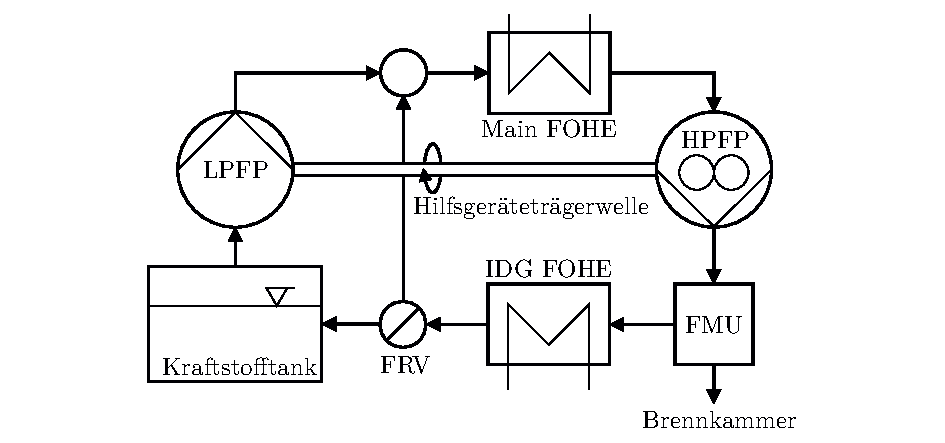
\includegraphics[width=1\linewidth]{4_Abbildungen/2_Hauptteil/Kraftstoffsystem Abbildungen/CFM56 Kraftstoffsystem 2.pdf}
  \caption{Kraftstoffsystems des CFM56-5B Triebwerks nach \cite{LinkeDiesinger.2014}}
  \label{fig:2.1}
\end{figure}
\FloatBarrier

Die in den Kraftstofftanks integrierten Boosterpumpen (in Abbildung \ref{fig:2.1} nicht abgebildet) versorgen die Triebwerke mit Kraftstoff. Im CFM56-5B Triebwerk wird der Kraftstoff zunächst von der Niederdruckpumpe in das Niederdrucksystem gefördert. Anschließend erfolgt eine Mischung mit warmem, rezirkuliertem Kraftstoff aus dem Hochdrucksystem. Nachdem der Kraftstoff in einem Wärmeübertrager für das Hauptölsystem weiter erwärmt wurde, durchläuft er den Kraftstofffilter und die Hochdruckpumpe.

Der Filter des CFM56-5B Triebwerks ist branchenüblich mit einem von einem Druckdifferenzsensor gesteuerten Bypass-Ventil ausgestattet, das im Falle einer Verstopfung aktiviert wird. Der Kraftstoffmassenstrom und -druck in die Brennkammer werden durch die Kraftstoffregeleinheit gesteuert, die im CFM56-5B Triebwerk auch als hydromechanische Einheit (engl.: Hydromechanical Unit, HMU) bezeichnet wird. Überschüssiger Kraftstoff durchläuft zunächst den Wärmeübertrager des Stromgenerator-Ölsystems und erreicht anschließend das Kraftstoff-Rückführventil (engl.: Fuel Return Valve, FRV). Je nach Öltemperatur bestimmt das Wärmemanagementsystem des CFM56-5B Triebwerks anhand eines Kennfeldes, welcher Kraftstoffmassenstrom in die Kraftstofftanks zurückgeleitet wird. Der restliche Kraftstoff wird in das Niederdrucksystem zurückgeführt. Die Kraftstofftemperatur wird vom Wärmemanagementsystem des CFM56-5B Triebwerk nicht berücksichtigt. \cite{Braunling.2015, LinkeDiesinger.2014}

\section{Wasserstoff-Kraftstoffsysteme}

Die Kraftstoffsysteme wasserstoffbetriebener Triebwerke müssen viele der gleichen Funktionen wie Kerosin-Kraftstoffsysteme erfüllen. Aufgrund der abweichenden Kraftstoffeigenschaften ergeben sich jedoch spezifische Herausforderungen. Da der Wasserstoff für Luftfahrtanwendungen in flüssiger, also kryogener Form bei niedrigen Temperaturen gespeichert wird, stellt die Vorkonditionierung eine besondere Herausforderung dar. Die Kombination aus niedrigeren Lagertemperaturen und der hohen spezifischen Wärmekapazität von Wasserstoff führt zu einem hohen Energiebedarf. \cite{Rompokos.2024, Sethi.2022}

Aus diesem Grund werden in der Literatur neben den aus konventionellen Kraftstoffsystemen bekannten Wärmeübertragern mit den Ölsystemen auch Wärmeübertrager innerhalb des thermodynamischen Kreisprozesses des Triebwerks untersucht (siehe Abbildung \ref{fig:2.2}). Diese sogenannten fortschrittlichen Kreisprozesse könnten nicht nur zusätzliche Wärmeeinträge in das Kraftstoffsystem liefern, sondern auch den Gesamtwirkungsgrad des Triebwerks steigern \cite{Tacconi.2023}.

\begin{figure}[ht]
\centering
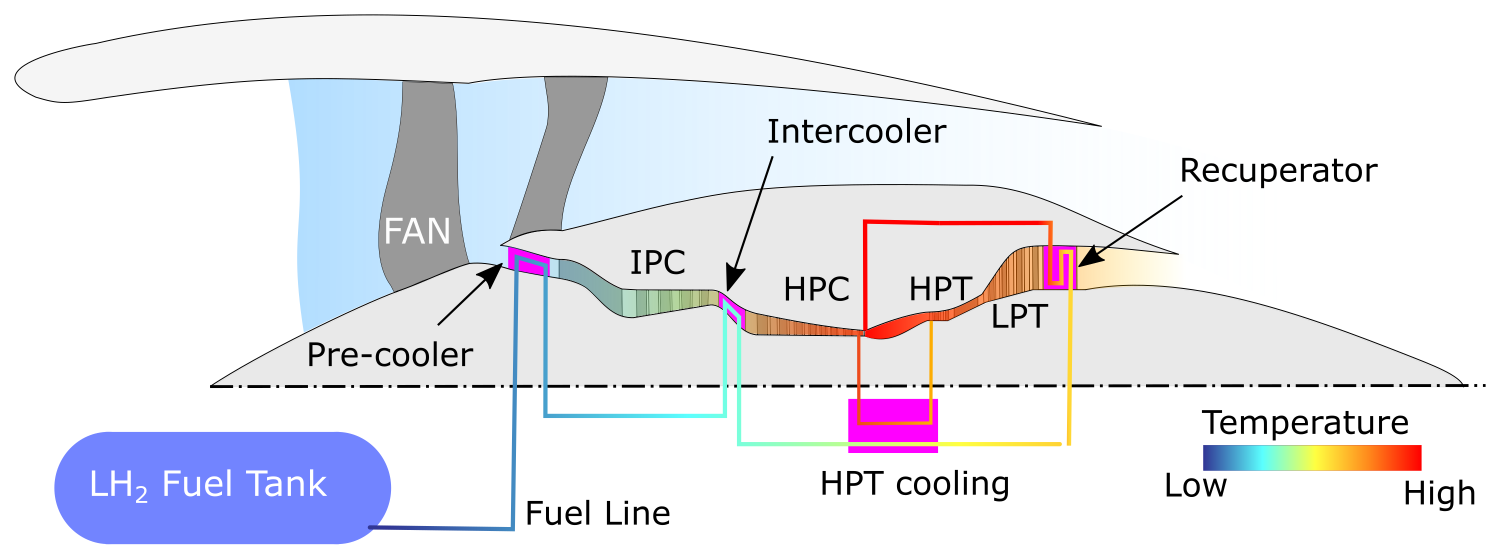
\includegraphics[width=0.75\linewidth]{4_Abbildungen/2_Hauptteil/Advanced Cycles.png}
  \caption{Wärmeübertrager fortschrittlicher Kreisprozesse \cite{Sethi.2022}}
  \label{fig:2.2}
\end{figure}
\FloatBarrier 

Zu den untersuchten fortschrittlichen Kreisprozessen zählen Vor-/Zwischenkühler, die durch geringere Eintrittstemperaturen der Luft in die Verdichter des Kerntriebwerks deren Arbeitsbedarf reduzieren \cite{Abedi.2022}. Wärmerückgewinnungssysteme im Abgas der Niederdruckturbine, sogenannte Rekuperatoren, senken die Abgastemperatur und erhöhen dadurch den Gesamtwirkungsgrad des Kreisprozesses \cite{Brewer.1991}. Eine Vorkühlung der Turbinenkühlluft in einem eigenen Wärmeübertrager könnte den benötigten Massenstrom an Kühlluft verringern und so den Turbinenwirkungsgrad steigern \cite{Brewer.1991}. Die Integration dieser Wärmeübertrager in den Kreisprozess des Triebwerks ist jedoch mit erheblichen finanziellen und technischen Risiken verbunden, weshalb ein Einsatz in der ersten Generation wasserstoffbetriebener Flugzeugtriebwerke als unwahrscheinlich gilt \cite{Rompokos.2024, Huete.2021}. 

Da sich diese Arbeit primär mit der Nachrüstung von kerosinbetriebenen Flugtriebwerken für die Nutzung mit Wasserstoff befasst, werden fortschrittliche Kreisprozesse nicht näher betrachtet. Das Wärmemanagement von Wasserstoff-Kraftstoffsystemen hält die Temperaturen der Ölsysteme innerhalb ihrer Betriebsgrenzen und stellt eine Mindesttemperatur des Kraftstoffs sicher. Im Folgenden werden mögliche Komponenten von Wasserstoff-Kraftstoffsystemen diskutiert und eine Kraftstoffsystemarchitektur aus der Literatur beschrieben.

\subsection{Kraftstoffpumpen}

Die Druckerhöhung des Kraftstoffs erfolgt bei den in der Literatur vorgeschlagenen Wasserstoff-Kraftstoffsystemen in zwei Schritten \cite{Ebrahimi.2024}. Für die Niederdruckpumpe wird eine redundante Ausführung in Form von mehreren im Kraftstofftank versenkten Kreiselpumpen vorgeschlagen. Die Niederdruckpumpen des Wasserstoff-Kraftstoffsystems übernehmen die Funktion der Boosterpumpen und der Niederdruckpumpe des Kerosin-Kraftstoffsystems. Aufgrund der physischen Distanz zu den Triebwerkswellen werden diese Pumpen elektrisch angetrieben \cite{Scholz.2003}. 

Für die finale Druckerhöhung gibt es in der Literatur unterschiedliche Ansätze. Das Pumpen von Wasserstoff im flüssigen Zustand erfordert vergleichsweise wenig Energie, jedoch sind Pumpen für kryogenen Wasserstoff aufgrund der unzureichenden Schmierwirkung des Kraftstoffs störanfällig. Bacic et al. \cite{BacicMarkoCoullJohn.2024} schlagen daher vor, den Kraftstoff nach erfolgter Verdampfung zu verdichten, um längere Wartungsintervalle zu ermöglichen. Für die Hochdruckpumpe beziehungsweise den Hochdruckverdichter ist sowohl ein Antrieb über die Hochdruckwelle als auch ein elektrischer Antrieb denkbar. Aufgrund der erforderlichen Druckverhältnisse bei hohem Schubbedarf, erfordert die Verdichtung im gasförmigen Zustand mehrere Verdichterstufen. Für die Druckerhöhung im flüssigen Zustand werden sowohl Kreiselpumpen als auch Verdrängerpumpen diskutiert \cite{Scholz.2003, Shaffer.2014}.

\subsection{Wärmeübertrager}

Neben den aus den Kerosin-Kraftstoffsystemen bekannten Wärmeübertragern mit den Ölsystemen bietet sich aufgrund des niedrigen Temperaturniveaus des flüssigen Wasserstoffs die Integration eines Wärmeübertragers mit dem Kabinen-Klimasystem (engl.: Environmental Control System, ECS) an \cite{Brewer.1991}. Das ECS wird mit Verdichter-Zapfluft versorgt, die vor ihrer Nutzung in der Kabine zunächst abgekühlt wird. In konventionellen Triebwerken wird hierfür ein mit Fan-Zapfluft gekühlter Wärmeübertrager eingesetzt. Durch einen Wärmeübertrager zwischen Wasserstoff und ECS kann der Fan-Zapfluftbedarf reduziert und zusätzliche Wärme für das Wasserstoff-Kraftstoffsystem gewonnen werden. 

Patrao et al. \cite{Patrao.2024} diskutieren die Problematik der Eisbildung in kryogenen Wärmeübertragern im Wasserstoff-Kraftstoffsystem. Ein möglicher Lösungsansatz ist die Rezirkulation des Wasserstoffs innerhalb des Kraftstoffsystems. Hierbei wird warmer Wasserstoff aus dem Hochdrucksystem vor den Eintritt in die betroffenen Wärmeübertrager rezirkuliert, um die Eintrittstemperatur des Wasserstoffs in die Wärmeübertrager so weit zu erhöhen, dass die luftseitigen Temperaturen des Wärmeübertragers stets oberhalb des Gefrierpunkts von Wasser bleiben \cite{Brewer.1991}. 

\subsection{Wärmemanagementsystem}

Das Wärmemanagementsystem von Wasserstoff-Kraftstoffsysteme unterscheidet sich in zwei Kernpunkten von konventionellen Kraftstoffsystemen. Zum einen ist es in der Regel nicht möglich, einen signifikanten Kraftstoffmassenstrom in die Kraftstofftanks rückzuführen, da der rückgeführte Wasserstoff wieder verflüssigt werden müsste. Eine Rückführung des Wasserstoffs für Zwecke des Wärmemanagements ist allerdings auch nicht erforderlich. Im Gegensatz zu Kerosin-Kraftstoffsystemen ist der Kraftstofftemperatur bei den Wasserstoff-Kraftstoffsystemen keine technische Obergrenze gesetzt. Im Gegenteil: Um Vereisungsprobleme aufgrund niedriger Kraftstofftemperaturen in der Brennkammer zu vermeiden, könnte neben der verfügbaren Abwärme auch der Einsatz weiterer Wärmequellen erforderlich sein. Als Alternative zu den zuvor diskutierten fortschrittlichen Kreisprozessen schlagen Palmer et al. \cite{PalmerChloeJWhurrJohnR.2024} vor, die für die Vorkonditionierung benötigte Wärme durch eine mit Fan-Zapfluft versorgte parallele Wasserstoffverbrennung bereitzustellen. Des Weiteren diskutiert der CRYOPLANE-Bericht \cite{Scholz.2003} die Erwärmung des Wasserstoffs im transienten Betrieb mit einer elektrischen Widerstandsheizung.

\subsection{Anordnung der Kraftstoffsystemkomponenten}

Brewer \cite{Brewer.1991} beschreibt in seinem Buch einen denkbaren Ansatz für Wasserstoff-Kraftstoffsysteme. Abbildung \ref{fig:brewer} enthält einen schematische Darstellung der Anordnung der Kraftstoffsystemkomponenten des Kraftstoffsystems von Brewer.


\begin{figure}[ht]
\centering
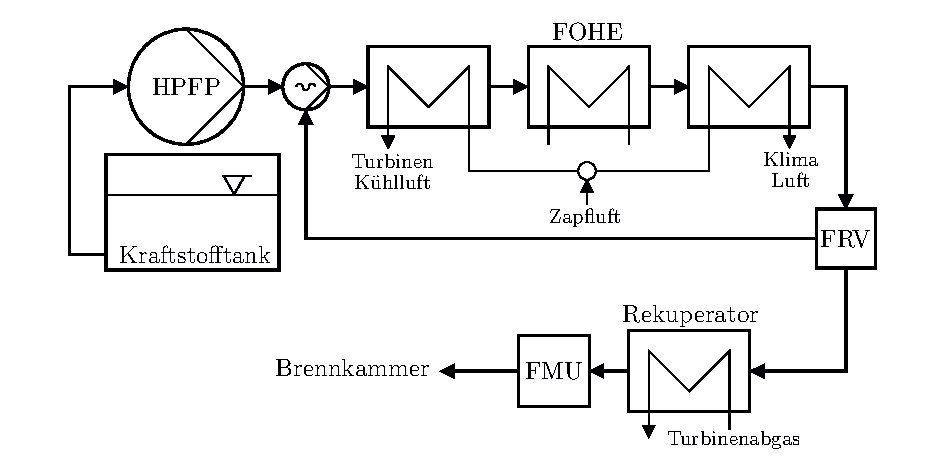
\includegraphics[width=1\linewidth]{4_Abbildungen/2_Hauptteil/Kraftstoffsystem Abbildungen/brewer.pdf}
  \caption{Wasserstoff-Kraftstoffsystem frei nach Brewer \cite{Brewer.1991}}
  \label{fig:brewer}
\end{figure}
\FloatBarrier 

Der flüssige Wasserstoff wird unter Überdruck in einem in die Zelle des Flugzeugs integrierten Kraftstofftank  gelagert. Eine elektrisch angetriebenen Kreiselpumpe fördert den Kraftstoff aus dem Tank in das Triebwerk. Im Triebwerk wird der flüssige Wasserstoff von der Hochdruckpumpe über den Brennkammerdruck gefördert. Im Anschluss an die Hochdruckpumpe, die ebenfalls als Kreiselpumpe ausgeführt ist, wird der geförderte Wasserstoff in einer Strahlpumpe als Treibmedium verwendet, um den rezirkulierten gasförmigen Wasserstoff zu fördern. Der rezirkulierte Wasserstoff gibt Wärme an den flüssigen Wasserstoff ab, wodurch dieser verdampft und auf eine Temperatur von \SI{200}{K} erwärmt wird. 

Der gemischte Wasserstoffstrom durchläuft wird anschließend in einer Reihe von Wärmeübertragern durch die Turbinenkühlluft, das Hauptölsystem und die Klimaluft erwärmt. Hinter den Wärmeübertragern wird der rezirkulierte Massenstrom in einem Kraftstoff-Rückführventil abgezapft. Der verbleibende Kraftstoff durchläuft anschließend einen Rekuperator, der den Wasserstoff auf eine Temperatur von \SI{677}{K} erhitzt. Abschließend wird der Wasserstoff durch die Kraftstoffregeleinheit in die Brennkammer geleitet.
%==============================================================================
\chapter{Stand der Technik}\label{chap:standdertechnik}
%==============================================================================

Mehrere Autoren haben bereits Kraftstoffsysteme für Fluggasturbinen modelliert. Im Folgenden werden ausgewählte Modellierungsansätze aus der Literatur erläutert. Für die Modellierung von Kraftstoff- und Wärmemanagementsystemen werden insbesondere physikbasierte Ansätze verwendet.

Mawid et al. \cite{Mawid.1998} haben eine Simulationssoftware für thermo-hydraulische Systeme angepasst, um  Kerosin-Kraftstoffsysteme zu simulieren. Der Schwerpunkt der Arbeit liegt auf der akkuraten Modellierung des Verhaltens der Hochdruckpumpe.

Bodie et al. \cite{Bodie.2010} haben die Wärmemanagementsysteme eines Flugzeugs, einschließlich des Kraftstoffsystems, durch ein Netzwerkmodell (engl.: lumped element model) in MATLAB Simulink modelliert. Die Autoren empfehlen in der frühen Entwicklungsphase den Einsatz von Ersatzmodellen mit verringerter Genauigkeit und geringem Rechenaufwand, um die Festlegung der Modelltopologie zu beschleunigen.

German \cite{German.2012} hat mit einem physikbasierten Ansatz die Auswirkungen der Kraftstoffrückführung auf die Temperaturen des Kraftstoff in den Kraftstofftanks modelliert. Die Modellierung kann aufgrund ihres geringen Detailgrads schon früh in der Entwicklungsphase genutzt werden, um die Anforderungen an das Wärmemanagementsystem abzuschätzen.

Sun et al. \cite{Sun.2019} haben die Modellierungen des Kraftstoffsystems und des Ölsystems eines kerosinbetriebenen Turbofantriebwerks in MATLAB Simulink gekoppelt. Die gekoppelte Modellierung der Systeme ermöglicht eine akkurate Abbildung des Systemverhaltens auch unter untypischen Betriebsbedingungen.

Sciatti et al. \cite{Sciatti.2022} haben ein Kerosin-Kraftstoffsystem mit einem physikbasierten Ansatz in MATLAB Simulink modelliert. Im Mittelpunkt der Arbeit steht die Interaktion zwischen der Hochdruckpumpe und der Kraftstoffregeleinheit. Das Wärmemanagementsystem wird hingegen nicht betrachtet. 

Bisherige Arbeiten in diesem Gebiet konzentrierten sich vor allem auf die dynamischen Interaktionen des Kraftstoffsystems mit anderen Systemen. Diese Arbeit hingegen betrachtet ausschließlich das Kraftstoffsystem selbst und blendet transientes Systemverhalten aus. Der Fokus liegt auf der Ermittlung der Leistungs- und Wärmebedarfe von Kraftstoffsystemen in erster Größenordnung, sodass diese bei der Leistungsrechnung fortschrittlicher Fluggasturbinen berücksichtigt werden können. So soll insbesondere eine Vergleichbarkeit zwischen wasserstoff- und kerosinbetriebenen Fluggasturbinen ermöglicht werden. Hierfür wird die Energiebilanz der Modelle der einzelnen Komponenten in einem analytischen, physikbasierten Ansatz gelöst. 	
%==============================================================================
\chapter{Methodik}
\label{chap:methodik}
%==============================================================================
Ziel dieser Arbeit ist die Entwicklung einer Methode für die Modellierung von Kraftstoffsystemen für Fluggasturbinen, um deren Vorauslegung zu unterstützen. Insbesondere wird angestrebt, eine Vergleichbarkeit des Wärme-/Leistungsbedarfs zwischen Wasserstoff- und Kerosin-Kraftstoffsystemen zu ermöglichen. 

Zunächst werden die Stoffmodelle für Kerosin und Wasserstoff erläutert. Anschließend werden die für die Modellierung der Kraftstoffsysteme erforderlichen Komponentenmodelle definiert. Im nächsten Schritt wird das Kraftstoffsystem des kerosinbetriebenen CFM56-5B Triebwerks aus den Komponentenmodellen nachgebildet und mögliche Architekturen für Wasserstoff-Kraftstoffsysteme erarbeitet. Abschließend wird der Lösungsalgorithmus der Modellierung erläutert.

\section{Annahmen und Vereinfachungen}

Um einen Kompromiss zwischen Detailtiefe, Genauigkeit und Rechenaufwand zu finden, werden in dieser Arbeit mehrere Vereinfachungen verwendet. Insbesondere gelten die betrachteten Modelle lediglich für den stationären Fall. Transientes Systemverhalten wird nicht betrachtet. 

Zudem wird in den für die Modellierung relevanten Querschnitten der Kraftstoffsysteme von vernachlässigbaren Geschwindigkeiten, beziehungsweise kinetischen Energien ausgegangen. Innerhalb der modellierten Turbomaschinen ist diese Annahme nicht gültig, jedoch beschränkt sich die Modellierung auf die Erfassung der Stoffgrößen in den Leitungen zwischen den jeweiligen Komponenten. Bei einer konservativ abgeschätzten Machzahl in den Leitungen von $Ma_L=0.1$ und mit dem Isentropenexponenten $\kappa_{\mathrm{H}_2} = 1.4$ beträgt das mit der Isentropenbeziehung berechnete total zu statische Temperaturverhältnis  $\frac{T_{t,L}}{T_L}$

\begin{equation}\label{Eq:mach}
	\frac{T_{t,\mathrm{L}}}{T_\mathrm{L}}=1+\frac{\kappa_{\mathrm{H}_2}-1}{2}Ma_\mathrm{L}^2
\end{equation}

lediglich $1,002$. Unter Annahme eines maximalen Wasserstoffmassenstroms von \SI{0.731}{\kg\per\s} bei einer Temperatur von \SI{300}{\K} beträgt der maximale Leitungsdurchmesser \SI{69}{\milli\m}, was als unkritisch eingestuft wird. Somit gilt die Annahme 

\begin{equation}\label{Eq:ts}
	T_s=T_t=T,\quad h_s=h_t=h,\quad p_s=p_t=p\,.
\end{equation}

\section{Stoffmodelle}

Die Modellierung der Kraftstoffsysteme erfordert Stoffmodelle, um thermodynamische Zustandsgrößen wie die spezifische Enthalpie und Entropie in Abhängigkeit von Temperatur und Druck der Kraftstoffe zu bestimmen. In diesem Abschnitt werden die für Kerosin und Wasserstoff verwendeten Stoffmodelle erläutert.

\subsection{Wasserstoff Stoffmodell}

Wasserstoff besteht aus zwei unterschiedlichen Kernspin-Isomeren, Parawasserstoff und Orthowasserstoff. Da sich die beiden Spin-Isomer in ihrer Wärmekapazität bei niedrigen Temperaturen unterscheiden, muss das Stoffmodell das Verhältnis der Kern-Isomer berücksichtigen. Bei Temperaturen oberhalb von \SI{200}{\K} liegen die Isomere im thermischen Gleichgewicht in einem Verhältnis von 3:1 zwischen Ortho- und Parawasserstoff vor. Flüssiger Wasserstoff besteht im Gleichgewichtszustand hingegen aus nahezu purem Parawasserstoff (Siehe Abbildung \ref{fig:spin}). In Abwesenheit eines Katalysators wird der Gleichgewichtszustand nur langsam erreicht. Es ist daher davon auszugehen, dass der ursprünglich kryogen gelagerte Wasserstoff im gesamten Kraftstoffsystem nahezu vollständig in Form von Parawasserstoff vorliegt. Für die Parametrierung des Stoffmodells wird daher eine Zusammensetzung aus purem Parawasserstoff angenommen. \cite{Buntkowsky.2022}

\begin{figure}[ht]
	\centering
	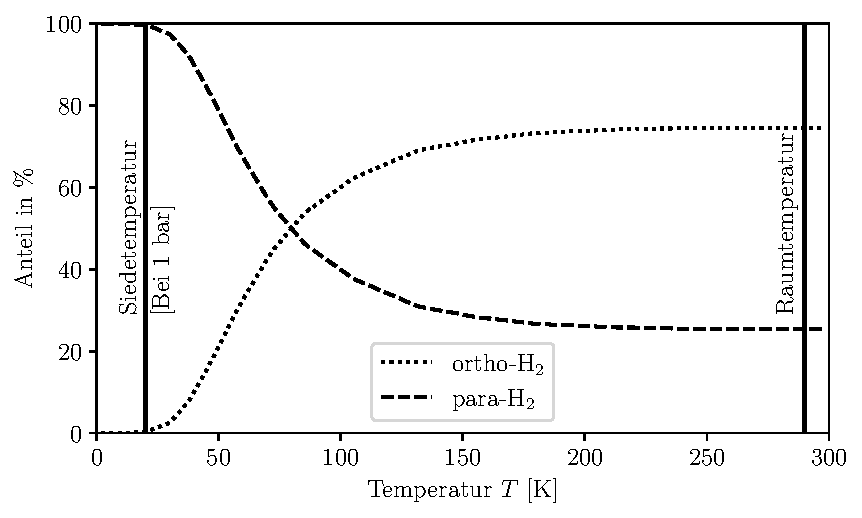
\includegraphics[width=1\linewidth]{4_Abbildungen/2_Hauptteil/spin.pdf}
	\caption{Wasserstoff Kernspin-Isomer Anteile nach \cite{Buntkowsky.2022}}
	\label{fig:spin}
\end{figure}
\FloatBarrier 

Für die Berechnung der thermodynamischen Zustandsgrößen von Parawasserstoff, wird ein am Institut für Strahlantriebe und Turbomaschinen (IST) entwickeltes Stoffmodell weiterentwickelt. Das Stoffmodell basiert auf einem von Leachman et al. \cite{Leachman.2017} beschriebenen Ansatz, der die Zustandsgrößen in Abhängigkeit der Helmholtz-Energie, die auch als freie Energie bekannt ist, setzt. Leachman et al. berechnen die entdimensionierte Helmholtz-Energie $\alpha$ 

\begin{equation}\label{Eq:free-energy}
	\alpha(\delta, \tau) = \alpha^0(\delta, \tau) + \alpha^r(\delta, \tau)
\end{equation}

als Summe der Idealgaskomponente $\alpha^0$ und des Anteils aufgrund von Kompressibilität $\alpha^r$. Hierbei gelten folgende Definitionen der entdimensionierten Helmholtz-Energie $\alpha$ und der entdimensionierten Variablen $\delta$ und $\tau$

\begin{equation}
	\alpha = \frac{a}{RT}, \quad \delta = \frac{\rho}{\rho_c}, \quad \tau = \frac{T_c}{T} \,
\end{equation}

in Abhängigkeit der spezifischen freien Energie $a$ und den Zustandsgrößen $\rho_c, T_c$ im kritischen Punkt.  Leachman et al. berechnen die Idealgaskomponente der entdimensionierten freien Energie $\alpha^0$

\begin{equation}\label{Eq:free-energy-idealgas}
	\alpha^0(\tau,\delta)=ln(\delta)+(a_0-1)\mathrm{ln}(\tau)+a_1+a_2\tau-\sum_{i=3}^{m}a_i\frac{(\frac{T_c}{\tau})^{k_i}}{k_i(k_i+1)}+\sum_{i=m+1}^{n}a_i\mathrm{ln}\left(1-e^{\frac{-k_i\tau}{T_c}}\right) \,
\end{equation}

mit einer semi-empirischen Zustandsgleichung, wobei die empirisch bestimmten Koeffizienten $a_i$ und $k_i$ verwendet werden. Die Zustandsgleichung für den Anteil an der entdimensionierten freien Energie aufgrund von Kompressibilitätseffekten $\alpha^r$

\begin{equation}\label{Eq:free-energy-compressibility}
	\alpha^r(\tau,\delta)=\sum_{i=1}^{l}N_i\delta^{d_i}\tau^{t_i}+\sum_{i=l+1}^{m}N_i\delta^{d_i}\tau^{t_i}e^{-\delta^{p_i}}+\sum_{i=m+1}^{n}N_i\delta^{d_i}\tau^{t_i}e^{-\phi_i(\delta-D_i)^2-\beta_i(\tau-\gamma_i)^2)}
\end{equation}

orientiert sich an theoretischen und praktischen Abwägungen. Die in Gleichung \ref{Eq:free-energy-compressibility} enthaltenen Koeffizienten $N_i, d_i, t_i, p_i, \phi_i, D_i, \beta_i$ und $\gamma_i$ werden experimentell bestimmt. Da die freie Energie eine Funktion von Dichte und Temperatur ist, der Zustand in dieser Arbeit hingegen in Form von Druck und Temperatur bekannt ist, wird zunächst die Dichte des Wasserstoffs berechnet. Um die Dichte zu berechnen wird die Zustandsfunktion für den Druck $p$

\begin{equation}\label{Eq:pressure-guess}
	p=\rho RT\left(1+\delta\frac{\partial\alpha^r}{\partial\delta}(\delta, \tau)\right)
\end{equation}

iterativ mit dem Newton-Raphson-Verfahren gelöst. Die Ableitung des inkompressiblen Anteils der freien Energie nach der entdimensionierten Dichte $\frac{\partial\alpha^r}{\partial\delta}$ wird aus Gleichung \ref{Eq:free-energy-compressibility} hergeleitet. Mit Dichte und Temperatur beziehungsweise deren entdimensionierten Äquivalenten ist es möglich die freien Energien und die Ableitungen der freien Energien nach $\delta$ und $\tau$ zu berechnen und das Stoffmodell ist somit eindeutig bestimmt. Diese Werte liefern die Grundlage für die Berechnung der thermodynamischen Zustandsgrößen mit den in Tabelle \ref{Tab:thermodynamic_properties_h2} definierten Zustandsgleichungen.

\begin{table}[ht]
	\centering
	\caption{Formeln für thermodynamische Zustandsgrößen von Wasserstoff}
	\begin{tabular} {|l|c|c|} \hline%
		\multicolumn{2}{|c|}{Zustandsgröße}  & Formel\\ \hline\hline%
		spezifische Enthalpie &$h$ 		  & $RT(\tau\frac{\partial\alpha}{\partial\tau}+\delta\frac{\partial\alpha^r}{\partial\delta}+1)$ \\ \hline%
		spezifische Entropie& $s$ 		      &  $R(\tau\frac{\partial\alpha}{\partial\tau}-\alpha)$\\ \hline%
		spezifische isochore Wärmekapazität &$c_v$ 	    &  $-R\tau^2\frac{\partial^2\alpha}{\partial\tau^2}$\\ \hline%		
		spezifische isobare Wärmekapazität &$c_p$        &  $c_v+R\frac{\left(1+\delta\frac{\partial\alpha^r}{\partial\delta}-\delta\tau\frac{\partial^2\alpha^r}{\partial\delta\partial\tau}\right)^2}{1+2\delta\frac{\partial\alpha^r}{\partial\delta}+\delta^2\frac{\partial^2\alpha^r}{\partial\delta^2}}$\\ \hline%
	\end{tabular}	
	\label{Tab:thermodynamic_properties_h2}%
\end{table}
\FloatBarrier 

\subsection{Kerosin Stoffmodell}

Die Modellierung von Kerosin beziehungsweise Jet-A ist grundsätzlich mit Unsicherheit behaftet, da die Spezifikation des Kraftstoffs vergleichsweise große Abweichungen der Eigenschaften zulässt. Outcalt et al. \cite{Outcalt.2009} haben die Dichte von drei unterschiedlichen Proben an Jet-A Kraftstoff für Temperaturen zwischen \SI{270}{\K} und \SI{470}{\K} und Drücke zwischen \SI{83}{\kilo\Pa} und \SI{30}{\mega\Pa} gemessen und haben Abweichungen von bis zu $4\,\%$ zwischen den Dichten der Proben ermittelt.

Da Kerosin kein Reinstoff, sondern eine Mischung von Kohlen-Wasserstoffverbindungen mit unterschiedlichen Kettenlängen ist, kann ein Kerosin Stoffmodell nicht mit demselben Ansatz wie das Wasserstoff Stoffmodell entwickelt werden. Stattdessen wird ein empirisches Stoffmodell verwendet, das von McBridge et al. \cite{McBridge.2002} vorgeschlagen wurde. Die Autoren haben generische empirische Formeln in Form von Polynomen für die Enthalpie, Entropie und isobare Wärmekapazität aufgestellt und anhand experimenteller Messungen der Zustandsgrößen für 2000 Spezies, inklusive Jet-A Kraftstoff, mit den Koeffizienten $a_i$ und $b_i$ parametriert. Tabelle \ref{Tab:thermodynamic_properties_jeta} liefert einen Überblick über die verwendeten Zustandsgleichungen.

\begin{table}[ht]
	\centering
	\caption{Thermodynamische Zustandsgrößen von Jet-A Kraftstoff nach 
		\cite{McBridge.2002}}
	\begin{tabular} {|l|c|l|} \hline%
		\multicolumn{2}{|c|}{Zustandsgröße}  & Formel\\ \hline\hline%
		spezifische Enthalpie &$h$ & $R(a_1T^{-2}+a_2T^{-1} +a_3$ \\ 
		& & $+a_4T+a_5T^2+a_6T^3+a_7T^4)$\\ \hline
		spezifische Entropie& $s$ &  $R(-a_1T^{-1}+a_2ln(T)+a_3T$\\ 
		& & $+\frac{a_4T^2}{2}+\frac{a_5T^3}{3}+\frac{a_6T^4}{4}+\frac{a_7T^5}{5}+b_1)$\\ \hline
		spezifische isobare Wärmekapazität &$c_p$ &  $R(-\frac{a_1T^{-2}}{2}-a_2T^{-1}+a_3ln(T)+ a_4T$\\ 
		& & $+\frac{a_5T^{2}}{2}+\frac{a_6T^{3}}{3}+\frac{a_7T^{4}}{4}+b_2)$\\ \hline
	\end{tabular}	
	\label{Tab:thermodynamic_properties_jeta}%
\end{table}
\FloatBarrier 

Da eine Berechnung der Dichte mit demselben Ansatz nicht möglich ist, werden in dieser Arbeit stattdessen von Outcalt et al. \cite{Outcalt.2009} gemessenen Datenpunkte interpoliert. Als Datengrundlage wird die Probe "Jet-A 4658" verwendet, da sie von den Autoren als die repräsentativste der Proben erachtet wird. Für die Interpolation werden die vier angrenzenden Datenpunkte herangezogen. Zunächst wird die Dichte für den Druck interpoliert, da die Autoren die Dichte für uneinheitliche Druckschritte gemessen haben. Abschließend werden die druck-interpolierten Punkte für die Temperatur interpoliert. 

% Für die Berechnung der Dichte $\rho(T,p)$, werden die vier angrenzenden gemessenen Dichten $\rho(T_\mathrm{N},p_{\mathrm{N,n}})$, $\rho(T_\mathrm{N},p_{\mathrm{N,h}})$, $\rho(T_\mathrm{H},p_{\mathrm{H,n}})$ und $\rho(T_\mathrm{H},p_{\mathrm{H,h}})$ benötigt. Bei der Extrapolation werden stattdessen Messwerte der jeweils zwei nächsthöheren Temperaturen als Stützstellen verwendet. Da Outcalt et al. die Dichte für einheitliche Temperaturschritte, aber uneinheitliche Druckschritte gemessen haben, werden zunächst die Dichten $\rho(T_\mathrm{H}, p)$ und $\rho(T_\mathrm{N}, p)$ 

% \begin{equation}\label{Eq:pressure-interp}
	%\rho(T_i, p)= \rho(T_i, p_{i,\mathrm{n}}) + \frac{\rho(T_i, p_{i,\mathrm{h}})-\rho(T_i, p_{i,\mathrm{n}})}{p_{i,\mathrm{h}}-p_{i,\mathrm{n}}}(p-p_{i,\mathrm{n}}) 
%\end{equation}

%für den Druck interpoliert. Abschließend wird die Dichte $\rho(T,p)$

%\begin{equation}\label{Eq:temperature-interp}
	%\rho(T, p)= \rho(T_\mathrm{N}, p) + \frac{\rho(T_\mathrm{H}, p)-\rho(T_\mathrm{N}, p)}{T_\mathrm{H}-T_\mathrm{N}}(T-T_\mathrm{N}) 
%\end{equation}

%für die Temperatur interpoliert. 


\section{Modellierung der Komponenten}

Im Folgenden werden die Modellierungen der verschiedenen Kraftstoffsystem-Komponenten erläutert. Neben Modellen für Verdichter und Pumpen wird ein Modell für Wärmeübertrager benötigt. Für die Modellierung der Wasserstoff-Kraftstoffsysteme ist zusätzlich ein Modell für parallele Wasserstoffverbrennung in einer Nebenbrennkammer erforderlich. 

\subsection{Pumpen und Verdichter}

Sämtliche Verdichter- und Pumpentypen werden durch die Definition des isentropen Wirkungsgrad $\eta_s$

\begin{equation}\label{Eq:isentropic}
	\eta_s=\frac{h_2-h_1}{h_{2,s}-h_1}
\end{equation}

modelliert. Dabei werden neben dem isentropen Wirkungsgrad auch der Austrittsdruck $p_2$, der Eintrittsdruck $p_1$, die Eintrittstemperatur $T_1$ und somit über das Stoffmodell die spezifische Eintrittsenthalpie $h_1(T_1, p_1)$ sowie die spezifische Eintrittsentropie $s_1(T_1, p_1)$ als bekannt vorausgesetzt. Die Austrittstemperatur des reversiblen Prozesses $T_{2,s}$ wird iterativ mit der spezifischen Eintrittsentropie $s_1$ und dem Austrittsdruck $p_2$ bestimmt. Die Temperatur der nächsten Iteration wird mit der idealen Zustandsgleichung für die Entropie und der spezifischen isobaren Wärmekapazität $c_p(T_1,p)$ geschätzt 

\begin{equation}\label{Eq:entropy}
	s(T_2,p)-s(T_1, p)=\cancel{s(T_0,p_0) - s(T_0,p_0)} + c_p(T_1,p) ln\left(\frac{T_2}{T_1}\right) - {\cancel{\overbrace{R ln\frac{p}{p}}^{\substack{\text{Nur bei } \\ \text{idealem Gas}}}}}\,.
\end{equation}


Aus der Austrittstemperatur $T_{2,s}$ folgt direkt die spezifische Austrittsenthalpie $h_{2,s}$ des reversiblen Prozesses und somit durch Gleichung \ref{Eq:isentropic} auch die spezifische Austrittsenthalpie $h_2$ des realen Prozesses. In einem weiteren Iterativen Prozess wird mit dem Austrittsdruck $p_2$ und der spezifischen Austrittsenthalpie $h_2$ die Austrittstemperatur $T_2$ berechnet. Auch hier wird das ideale Stoffmodell verwendet, um Werte für die Austrittstemperatur zu schätzen

\begin{equation}\label{Eq:enthalpy}
	h(T_2,p)-h(T_1,p)=\cancel{h(T_0,p_0) - h(T_0,p_0)} + c_p(T_1,p)(T_2 - T_1) - {\cancel{\overbrace{v(p-p)}^{\substack{\text{Nur bei idealer} \\ \text{Flüssigkeit}}}}}\,.
\end{equation}

Abschließend wird mit der Energiebilanz um die Pumpe beziehungsweise den Verdichter die Leistung $P$ 

\begin{equation}\label{Eq:power}
	P=\dot{m}(h_2-h_1)
\end{equation}

bestimmt, die benötigt wird, um den Kraftstoffmassenstrom $\dot{m}$ zu fördern.

\subsection{Wärmeübertrager}

Eine Auslegungsrechnung der Wärmeübertrager wird in dieser Arbeit nicht angestrebt. Es gilt jedoch die Randbedingung, dass die Wärmequelle eines Wärmeübertragers in jedem Schnitt ein höheres Temperaturniveau als der zu erwärmende Kraftstoffmassenstrom aufweist. Anhand des $\dot{Q}-T$ Diagramms (Beispiel siehe Abbildung \ref{fig:hx}) kann festgestellt werden, ob über den gesamten Wärmeübertrager eine minimale Temperaturdifferenz $\Delta T_{min}$ zwischen Wärmequelle und Kraftstoffstrom eingehalten werden kann.


\begin{figure}[ht]
	\centering
	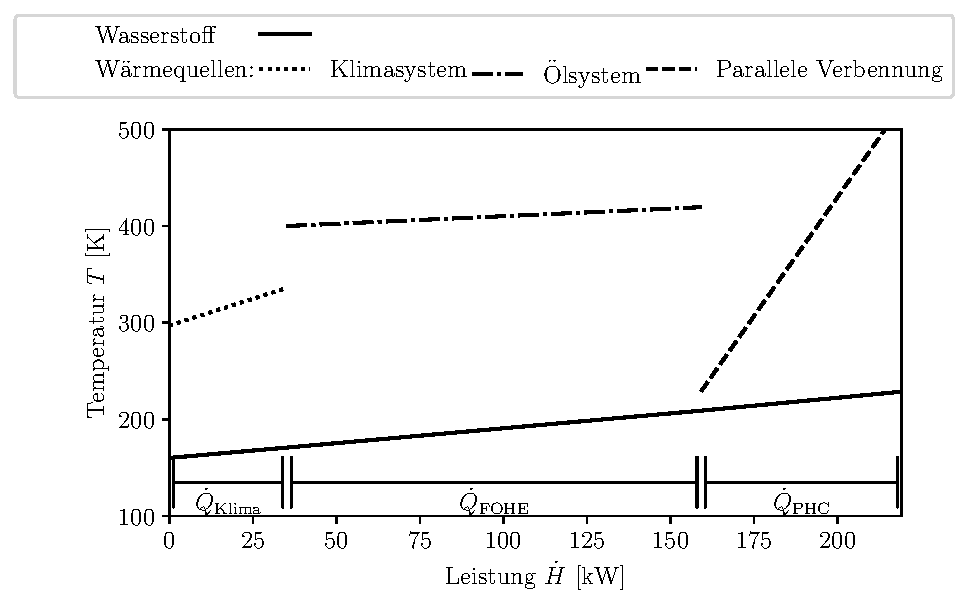
\includegraphics[width=1\linewidth]{4_Abbildungen/2_Hauptteil/hx.pdf}
	\caption{schematisches Wärmestromdiagramm eines Kraftstoffsystems}
	\label{fig:hx}
\end{figure}
\FloatBarrier 

Aus dem Eintrittszustand des Kraftstoffs in den Wärmeübertrager $T_1, p_1$ ergibt sich die spezifische Enthalpie des Kraftstoff im Eintritt in den Wärmeübertrager $h_1$. Die spezifische Austrittsenthalpie $h_2$

\begin{equation}\label{Eq:energy-hx}
	h_2=h_1 +q=h_1+\frac{\dot{Q}}{\dot{m}}
\end{equation}

erschließt sich direkt aus der Energiebilanz der Kraftstoffseite des Wärmeübertragers mit dem Wärmestrom $\dot{Q}$ und dem Kraftstoffmassenstrom $\dot{m}$. Über den Wärmeübertrager besteht infolge von Strömungsverlusten ein Druckverhältnis $\pi$. Der Austrittsdruck $p_2$

\begin{equation}\label{Eq:pressuredrop}
	p_2 = p_1 \pi
\end{equation}

fällt somit geringer als der Eintrittsdruck aus. Im Rahmen dieser Arbeit wird für das Druckverhältnis $\pi$ ein konstanter Wert angenommen. Abschließend wird erneut Gleichung \ref{Eq:enthalpy} eingesetzt, um iterativ die Austrittstemperatur $T_2$ des Kraftstoffs aus dem Wärmeübertrager zu bestimmen.

\subsection{Kraftstoffmischung}

In der Kraftstoffmischung werden die Kraftstoffmassenströme $\dot{m}_{1,\mathrm{\rom{1}}}$ und $\dot{m}_{1,\mathrm{\rom{2}}}$, mit demselben Eintrittsdruck $p_1$, aber unterschiedlichen Eintrittsenthalpien $h_{1,\mathrm{\rom{1}}}, h_{1,\mathrm{\rom{2}}}$ miteinander vermischt. Der Austrittsmassenstrom $\dot{m}_2$

\begin{equation}\label{Eq:mass}
	\dot{m}_2 = \dot{m}_{1,\mathrm{\rom{1}}}+\dot{m}_{1,\mathrm{\rom{2}}}
\end{equation}

berechnet sich aus der Massenbilanz um die Mischung. Die Austrittsenthalpie der Kraftstoffmischung 

\begin{equation}\label{Eq:energy-mix}
	h_{2} = \frac{\dot{m}_{1,\mathrm{\rom{1}}}h_{1,\mathrm{\rom{1}}}+\dot{m}_{1,\mathrm{\rom{2}}}h_{1,\mathrm{\rom{2}}}}{\dot{m}_2}
\end{equation}

wird mit der Energiebilanz um die Mischung bestimmt. Druckverluste in der Mischung werden vernachlässigt, somit entspricht der Austrittsdruck $p_2$, dem Eintrittsdruck $p_1$. Abschließend wird Gleichung \ref{Eq:enthalpy} erneut eingesetzt, um iterativ die Austrittstemperatur $T_2$ des gemischten Kraftstoffmassenstroms zu bestimmen. 

\subsection{Parallele Wasserstoffverbrennung}

In den Wasserstoff-Kraftstoffsystemen ist nicht ausreichend Abwärme vorhanden, um den Wasserstoff auf beliebige Brennkammer-Eintrittstemperatur zu erwärmen. In dieser Arbeit wird der potenzielle zusätzliche Wärmebedarf durch parallele Wasserstoffverbrennung in einer separaten Brennkammer aufgebracht. Diese Brennkammer wird mit Wasserstoff von der Kraftstoffregeleinheit und mit Fan-Zapfluft versorgt. Die Modellierung der parallelen Wasserstoffverbrennung berechnet diesen Mehrbedarf an Wasserstoff und Zapfluft. Unter Abwägung der angestrebten Detailtiefe werden die Prozesse der parallelen Wasserstoffverbrennung mit einer vereinfachten Energiebilanz um die Nebenbrennkammer und den dazugehörigen Wärmeübertrager modelliert 

\begin{equation}\label{Eq:phc}
	0 = \dot{m}_{\mathrm{H}_2, \mathrm{PHC}}\left(H_{u, \mathrm{H}_2} + \frac{1}{\beta_\mathrm{PHC}}c_{p,\mathrm{L}} T_{13} - \left(1+\frac{1}{\beta_\mathrm{PHC}}\right)c_{p,\mathrm{B}} T_\mathrm{B}\right)-\dot{Q}_\mathrm{PHC}\,.
\end{equation}

Für die Berechnung werden das Brennstoff-Luft-Verhältnis $\beta_\mathrm{PHC}$, die spezifischen isobaren Wärmekapazitäten von Luft $c_{p,\mathrm{L}}$ beziehungsweise dem Abgas $c_{p,\mathrm{B}}$ und die Fan-Zapflufttemperatur $T_{13}$ angenommen. Die Abgastemperatur hinter dem Wärmeübertrager $T_\mathrm{B}$ entspricht der Eintrittstemperatur des kalten Wasserstoffs in den PHC-Wärmeübertrager zuzüglich der Annäherungstemperatur $\Delta T$. Der benötigte Wasserstoffmassen $\dot{m}_{\mathrm{H}_2, \mathrm{PHC}}$ wie auch der Zapfluftbedarf $\dot{m}_\mathrm{Z} = \frac{\dot{m}_{\mathrm{H}_2, \mathrm{PHC}}}{\beta_\mathrm{PHC}}$ werden somit in Abhängigkeit des Wärmebedarfs $\dot{Q}_\mathrm{PHC}$ berechnet.

\section{Kerosin-Kraftstoffsystem}

Als Beispiel für ein Kerosin-Kraftstoffsystem wird das Kraftstoffsystem des CFM56-5B Triebwerks herangezogen. Die Kraftstoffsysteme der Triebwerke der jüngsten Generation, wie beispielsweise des Pratt \& Whitney PW1133G Triebwerks, sind in der vorhandenen Sachliteratur noch nicht ausführlich dokumentiert. Das andere in der Airbus A320ceo Familie eingesetzte Triebwerk, das International Aero Engines V2500-A5 Triebwerk, stellt eine denkbare Alternative dar. Das V2500-A5 Triebwerk ist jedoch nicht gut für eine Modellierung im Rahmen dieser Arbeit geeignet, da das Kraftstoffrückführventil des Triebwerks Funktionen aufweist, die in der verfügbaren Literatur nicht beschrieben sind \cite{LinkeDiesinger.2014}. Als verbleibendes Triebwerk der Airbus A320ceo Familie fällt die Wahl daher auf das CFM56-5B Triebwerk. 

\subsection{Systemarchitektur}

Die Modellierung des Kerosin-Kraftstoffsystems orientiert sich an der vereinfachten Darstellung des Kraftstoffsystems des CFM56-5B Triebwerks in Kapitel \ref{chap:grundlagen}. Eine schematische Darstellung der Modellierung des Kerosin-Kraftstoffsystems ist in Abbildung \ref{fig:Referenz} gegeben.

\begin{figure}[ht]
\centering
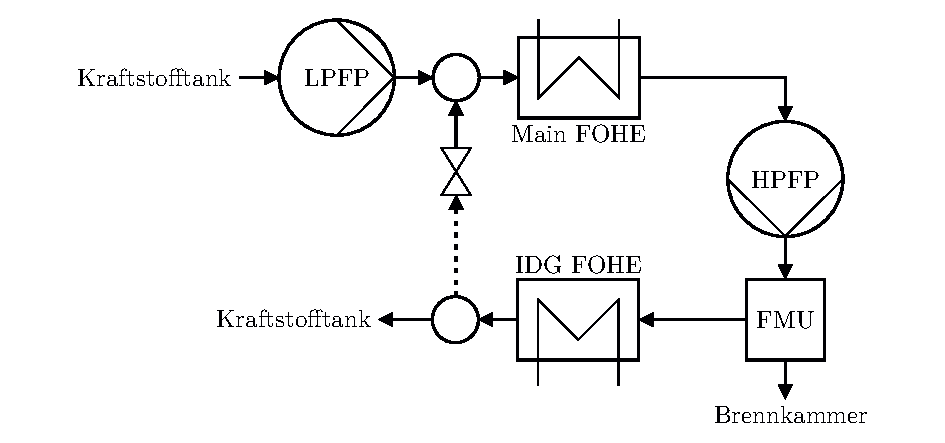
\includegraphics[width=1\linewidth]{4_Abbildungen/2_Hauptteil/Kraftstoffsystem Abbildungen/Referenz.pdf}
  \caption{Kerosin-Kraftstoffsystem}
  \label{fig:Referenz}
\end{figure}
\FloatBarrier 

In dieser Arbeit werden nur Komponenten, die sich innerhalb der Triebwerksgondel befinden, betrachtet. Die Kraftstofftanks und die darin befindlichen Boosterpumpen werden daher nicht modelliert. In der Modellierung wird stattdessen eine Versorgung der Niederdruckpumpe mit dem benötigten Kraftstoffmassenstrom, bei konstanten Eintrittsbedingungen $T_\mathrm{e}, p_\mathrm{e}$ angenommen. 

Die Niederdruckpumpe pumpt den Kraftstoff auf den Austrittsdruck $p_{\mathrm{LP}}$ mit dem isentropen Wirkungsgrad $\eta_{\mathrm{LP}}$ und einer Leistung von $P_{LP}$. Da die Modellierung vorwärts rechnet, ist es nicht möglich die spezifische Enthalpie $h_\mathrm{R}$ des rezirkulierten Kraftstoffs direkt innerhalb derselben Iteration zu integrieren. Stattdessen wird die in der vorherigen Iteration berechnete spezifische Enthalpie verwendet. Der rezirkulierte Kraftstoffmassenstrom $\dot{m}_\mathrm{R}$ wird so gewählt, dass die Brennkammer-Eintrittstemperatur $T_{\mathrm{BK}}$ eingehalten wird. 

Der gemischte Kraftstoffmassenstrom durchläuft anschließend den Wärmeübertrager für das Hauptölsystem und nimmt dabei die Wärme $\dot{Q}_{\mathrm{FOHE}}$ auf. Über diesen Wärmeübertrager liegt ein Druckverhältnis von $\pi_{\mathrm{FOHE}}$ an. Der erwärmte Kraftstoffmassenstrom wird nun in der Hochdruckpumpe mit dem isentropen Wirkungsgrad $\eta_{\mathrm{HP}}$ und einer Leistung $P_{\mathrm{HP}}$ gepumpt. Der Austrittsdruck der Hochdruckpumpe $p_{\mathrm{HP}}$ wird so gewählt, dass der Brennkammer-Eintrittsdruck $p_{\mathrm{BK}}$ erreicht wird.  Da es sich bei der Hochdruckpumpe um eine Verdrängerpumpe handelt und diese für den maximalen Kraftstoffverbrauch im Startfall dimensioniert wird, ist der geförderte Massenstrom im Reiseflug $\dot{m}_{\mathrm{HP}}$ vorgegeben. 

Vor dem Eintritt in die Kraftstoffregeleinheit werden in den Leitungen des Kraftstoffsystems auftretende Druckverluste $\Delta p_{\mathrm{L}}$  berücksichtigt. In der Kraftstoffregeleinheit wird der Kraftstoffmassenstrom für die Versorgung der Brennkammer $\dot{m}_{\mathrm{BK}}$ abgezweigt. In den Injektoren erfährt der Kraftstoff den Druckverlust $\Delta p_{\mathrm{inj}}$. 

Der übrige Kraftstoff durchläuft den Wärmeübertrager für das Ölsystem des Stromgenerators und nimmt dabei die Wärme $\dot{Q}_{\mathrm{IDG}}$ auf. Da der rezirkulierte Kraftstoff anschließend gedrosselt wird, wirken sich die Druckverluste dieses Wärmeübertragers nicht auf die Modellierung aus. Nachdem der letzte Wärmeübertrager durchlaufen wurde, wird die spezifische Enthalpie des rezirkulierten Massenstroms berechnet.

\subsection{Variablen und Parameter}

In dieser Arbeit werden unabhängige Variablen, abhängige Variablen, Zielgrößen und Parameter unterschieden. Die Zielgrößen der Modellierung des Kerosin-Kraftstoffsystems sind die Pumpenleistungen $P_{\mathrm{LP}}$ und $P_{\mathrm{HP}}$. Zu den unabhängigen Variablen des Kerosin-Kraftstoffsystems zählen der Brennkammerdruck $p_{\mathrm{BK}}$ und die Brennkammer-Eintrittstemperatur $T_{\mathrm{BK}}$. Der rezirkulierte Massenstrom $\dot{m}_\mathrm{R}$, dessen spezifische Enthalpie $h_\mathrm{R}$ und der Austrittsdruck der Hochdruckpumpe $p_{\mathrm{HP}}$ werden als abhängige Variablen modelliert. Tabelle \ref{Tab:referenz_params} zeigt die Parameter des Kerosin-Kraftstoffsystems.

\begin{table}[ht]
    \centering
	\caption{Parameter der Modellierung des Kerosin-Kraftstoffsystems}
	\begin{tabular} {|l|c|l|c|} \hline%
		\multicolumn{2}{|c|}{Parameter} & \multicolumn{2}{c|}{Parameter} \\ \hline\hline
        LPFP-Eintrittstemperatur & $T_\mathrm{e}$ & LPFP-Eintrittsdruck & $p_\mathrm{e}$ \\ \hline
        FOHE-Wärme & $\dot{Q}_{\mathrm{FOHE}}$ & FOHE-Druckverhältnis & $\pi_{\mathrm{FOHE}}$ \\ \hline   
        IDG-FOHE-Wärme  & $\dot{Q}_{\mathrm{IDG}}$ &  Brennkammermassenstrom & $\dot{m}_\mathrm{BK}$ \\ \hline
        LPFP-Austrittsdruck & $p_{\mathrm{LP}}$ & isentroper Wirkungsgrad LPFP & $\eta_{\mathrm{LP}}$ \\ \hline  
        HPFP-Massenstrom & $\dot{m}_{\mathrm{HP}}$ & isentroper Wirkungsgrad HPFP & $\eta_{\mathrm{HP}}$ \\ \hline
        Leitungs-Druckverluste & $\Delta p_{\mathrm{L}}$& Injektor-Druckverluste & $\Delta p_{\mathrm{inj}}$ \\ \hline
	\end{tabular}	
    \label{Tab:referenz_params}%
\end{table}
\FloatBarrier 

\section{Wasserstoff-Kraftstoffsystemarchitekturen}

Im Folgenden werden unterschiedliche Architekturen für Wasserstoff-Kraftstoffsysteme ausgearbeitet und beschrieben. Abschließend werden die für die Modellierung der Architekturen notwendigen Parameter erläutert. 

Insgesamt werden drei unterschiedliche Kraftstoffsystemarchitekturen betrachtet. Neben einem Kraftstoffsystem mit Hochdruckpumpe werden zwei Systeme mit Verdichter betrachtet. Die beiden Systeme mit Verdichter unterscheiden sich darin, wie sie den Wasserstoff verdampfen. Bei dem Kraftstoffsystem mit Verdampfer wird der Wasserstoff in einem Wärmeübertrager mit Kraftstoff aus dem Hochdrucksystem verdampft. Bei dem Kraftstoffsystem mit Vormischung wird eine geringe Menge Wasserstoff aus dem Hochdrucksystem vor den Verdichter rezirkuliert, um den Kraftstoff vollständig zu verdampfen.

\subsection{Systemarchitektur mit Hochdruckpumpe}

Im Gegensatz zum Kerosin-Kraftstoffsystem wird beim Wasserstoff-Kraftstoffsystem mit Hochdruckpumpe die Funktion der Pumpe nicht auf eine Hochdruck- und eine Niederdruckpumpe mit Wärmeübertragern dazwischen aufgeteilt. Eine Wärmezufuhr hinter einer möglichen Niederdruckpumpe würde den Wasserstoff schon vor der Hochdruckpumpe verdampfen. Die Lösung besteht darin, den Wasserstoff mit einer einzelnen Kreiselpumpe direkt in das Hochdrucksystem zu pumpen und erst daraufhin Wärme zuzuführen. Die hier diskutierte Kraftstoffsystemarchitektur basiert auf einem von Brewer diskutierten Kraftstoffsystem \cite{Brewer.1991}, jedoch wurden keine Wärmeübertrager mit der Turbinenkühlluft und dem Turbinenabgas vorgesehen. Stattdessen versorgt eine parallele Wasserstoffverbrennung den potenziellen Fehlbetrag zwischen dem Wärmebedarf und der verfügbaren Abwärme. Das Wasserstoff-Kraftstoffsystem mit Hochdruckpumpe ist in  Abbildung \ref{fig:pumpe} dargestellt.

\begin{figure}[ht]
\centering
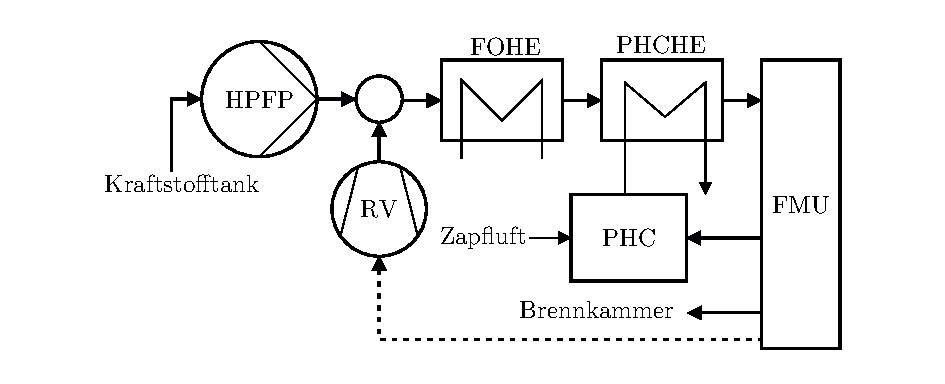
\includegraphics[width=1\linewidth]{4_Abbildungen/2_Hauptteil/Kraftstoffsystem Abbildungen/pump.pdf}
  \caption{Wasserstoff-Kraftstoffsystem mit Pumpe adaptiert aus \cite{Brewer.1991}}
  \label{fig:pumpe}
\end{figure}
\FloatBarrier 

Der Wasserstoff erreicht das Triebwerk im flüssigen Zustand mit dem Eintrittsdruck $p_\mathrm{e}$ und der Eintrittstemperatur $T_\mathrm{e}$ und wird direkt in der Hochdruckpumpe auf den Druck $p_{\mathrm{HP}}$ gepumpt, sodass der Brennkammer-Eintrittsdruck $p_{\mathrm{BK}}$ erreicht wird. Die Hochdruckpumpe arbeitet mit dem isentropen Wirkungsgrad $\eta_{\mathrm{HP}}$ und benötigt die Leistung $P_{\mathrm{HP}}$. 

Um die Druckverluste des rezirkulierten Kraftstoffs im Hochdrucksystem zu kompensieren, schlägt Brewer eine Strahlpumpe mit dem  Hochdruckpumpen-Kraftstoffmassenstrom als Treibmedium vor \cite{Brewer.1991}. Da in dieser Arbeit der rezirkulierte Massenstrom teilweise ein vielfaches des Hochdruckpumpen-Massenstroms beträgt, würde eine Strahlpumpe nicht hinnehmbare Druckverluste verursachen. Stattdessen wird ein Rezirkulationsverdichter (RV) modelliert. Der rezirkulierte Kraftstoffmassenstrom $\dot{m}_\mathrm{R}$ erreicht den Rezirkulationsverdichter mit der Temperatur $T_\mathrm{R}$ und dem Druck $p_\mathrm{R}$ und wird auf den Austrittsdruck der Hochdruckpumpe verdichtet. Der Rezirkulationsverdichter arbeitet mit dem isentropen Wirkungsgrad $\eta_\mathrm{RV}$ und benötigt die Leistung $P_\mathrm{VR}$. 

Der Hodchdruckpumpen-Massenstrom und der rezirkulierte Massenstrom werden anschließend miteinander vermischt. Der warme rezirkulierte Kraftstoff verdampft den flüssigen Kraftstoff aus der Hochdruckpumpe und erwärmt diesen auf die Wärmeübertrager-Eintrittstemperatur $T_\mathrm{W}$, um Vereisungen im Ölsystem zu vermeiden.

Auf den Wärmeübertrager mit dem Klimasystem, folgt der Wärmeübertrager mit dem Ölsystem. Der Einfachheit halber werden die beiden Wärmeübertrager in der Modellierung zusammengefasst. In den beiden Wärmeübertragern wird dem Kraftstoff in Summe die Wärme $\dot{Q}_{\mathrm{FOHE}}$ zugeführt. Über die beiden Wärmeübertrager liegt das Druckverhältnis $\pi_{\mathrm{FOHE}}$ vor. Der durch den Wärmeübertrager mit dem Klimasystem gesparte Fan-Zapfluftbedarf wird in der Modellierung nicht berücksichtigt. Um die angestrebte Brennkammer-Eintrittstemperatur $T_{\mathrm{BK}}$ zu erreichen, wird durch eine parallele Wasserstoffverbrennung (engl.: Parallel Hydrogen Combustion, PHC) in einem weiteren Wärmeübertrager (engl.: PHC Heat Exchanger, PHCHE) die zusätzliche Wärme $\dot{Q}_{\mathrm{PHC}}$ zugeführt. Dieser Wärmeübertrager verursacht das Druckverhältnis $\pi_{\mathrm{PHC}}$. 

Vor dem Eintritt in die Kraftstoffregeleinheit werden in den Leitungen des Kraftstoffsystems auftretende Druckverluste $\Delta p_\mathrm{L}$  berücksichtigt. Die Kraftstoffregeleinheit liefert den Kraftstoffmassenstrom $\dot{m}_{\mathrm{BK}}$ an die Hauptbrennkammer und die Brennkammer der parallelen Wasserstoffverbrennung. Der verbleibender Massenstrom $\dot{m}_\mathrm{R}$ mit der Temperatur $T_\mathrm{R}$ und dem Druck $p_\mathrm{R}$ wird rezirkuliert. Vor dem Eintritt in die Brennkammern erfährt der Wasserstoff die Injektor-Druckverluste $\Delta p_{\mathrm{inj}}$. 

\subsection{Systemarchitektur mit Verdampfer}

Die Architektur mit Verdichter und Verdampfer ist ähnlich wie das Kraftstoffsystem mit Hochdruckpumpe aufgebaut, jedoch wird anstatt der Hochdruckpumpe ein Hochdruckverdichter (engl.: High Pressure Fuel Compressor, HPFC) eingesetzt. Vor dem Eintritt in den Verdichter wird der Wasserstoff in einem Wärmeübertrager mit Wärme aus dem Hochdrucksystem verdampft. Abbildung \ref{fig:verdampfer} zeigt das Kraftstoffsystem mit Verdampfer.

\begin{figure}[ht]
\centering
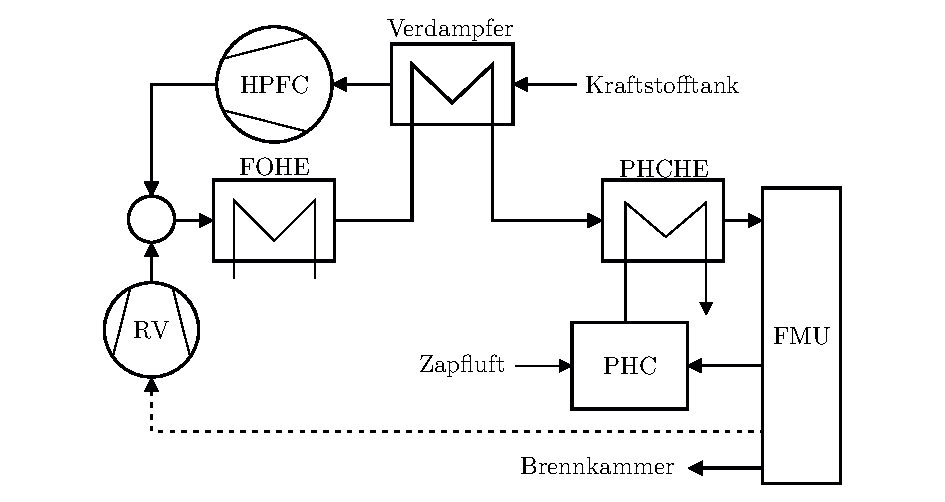
\includegraphics[width=0.85\linewidth]{4_Abbildungen/2_Hauptteil/Kraftstoffsystem Abbildungen/after.pdf}
  \caption{Wasserstoff-Kraftstoffsystem mit Verdichter und Verdampfer}
  \label{fig:verdampfer}
\end{figure}
\FloatBarrier 

Der Wasserstoff wird in dem Triebwerk zunächst in dem Verdampfer unter Zuführung des Wärmestroms $|\dot{Q}_\mathrm{V}|$ aus dem Hochdrucksystem gerade vollständig verdampft. Hierbei liegt über die Niederdruckseite des Wärmeübertragers das Druckverhältnis $\pi_{\mathrm{V,LP}}$ an. Der Hochdruckverdichter fördert den Wasserstoff mit dem Druck $p_{\mathrm{HP}}$ in das Hochdrucksystem, sodass der Brennkammer-Eintrittsdruck $p_{\mathrm{BK}}$ erreicht wird. Der Hochdruckverdichter arbeitet mit dem isentropen Wirkungsgrad $\eta_{\mathrm{HP}}$ und benötigt die Leistung $P_{\mathrm{HP}}$. 

Die Hochdruckseite gleicht dem Kraftstoffsystem mit Hochdruckpumpe mit dem einzigen Unterschied, dass zwischen dem Wärmeübertrager mit dem Ölsystem und dem Wärmeübertrager der parallelen Wasserstoffverbrennung die Hochdruckseite des Verdampfers durchlaufen wird. Hier wird die Wärme $\dot{Q}_\mathrm{V}$ an das Niederdrucksystem abgegeben und es liegt das Druckverhältnis $\pi_{\mathrm{V,HP}}$ an. Der Verdampfer wird auf der Hochdruckseite vor dem Wärmeübertrager mit der parallelen Wasserstoffverbrennung positioniert, um die maximale Wasserstofftemperatur zu mindern. Die geringere Maximaltemperatur ermöglicht eine geringere Abgastemperatur der parallelen Wasserstoffverbrennung und reduziert somit ihren Wasserstoffverbrauch.

\subsection{Systemarchitektur mit Vormischung}

Dieses Kraftstoffsystem hat das Alleinstellungsmerkmal, dass an zwei unterschiedliche Positionen Kraftstoff von der Kraftstoffregeleinheit rezirkuliert wird. Zum einen wie auch bei den anderen Wasserstoff-Kraftstoffsystemen über einen Rezirkulationsverdichter hinter den Hochdruckverdichter. Ein kleiner rezirkulierter Kraftstoffmassenstrom $\dot{m}_\mathrm{V}$ wird jedoch auf den Eintrittsdruck $p_\mathrm{e}$ gedrosselt und vor den Hochdruckverdichter rezirkuliert, um den aus dem Kraftstofftank geförderten Wasserstoff ohne den Einsatz zusätzlicher Wärmeübertrager zu verdampfen. Das Hochdrucksystem des Kraftstoffsystems mit Vormischung unterscheidet sich nicht von dem Kraftstoffsystem mit Hochdruckpumpe (Siehe Abbildung \ref{fig:vormischung}).

\begin{figure}[ht]
\centering
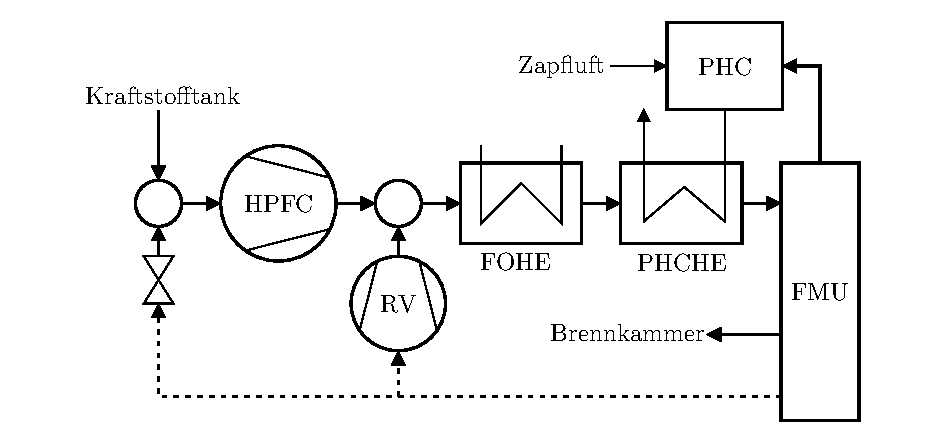
\includegraphics[width=1\linewidth]{4_Abbildungen/2_Hauptteil/Kraftstoffsystem Abbildungen/dual.pdf}
  \caption{Wasserstoff-Kraftstoffsystem mit Verdichter und Vormischung}
  \label{fig:vormischung}
\end{figure}
\FloatBarrier 

\subsection{Variablen und Parameter}

Die Zielgrößen der Wasserstoff-Kraftstoffsysteme sind die Pumpen-/Verdichterleistungen $P_{\mathrm{HP}}$ und $P_{\mathrm{RV}}$, sowie die Wärme der parallelen Wasserstoffverbrennung $\dot{Q}_\mathrm{PHC}$ und die damit assoziierten Wasserstoff- und Fan-Zapfluftbedarfe $\dot{m}_\mathrm{H\textsubscript{2}, PHC}$ und $\dot{m}_\mathrm{Z}$. Die unabhängigen Variablen der Modellierungen der Wasserstoff-Kraftstoffsysteme sind der Brennkammerdruck $p_{\mathrm{BK}}$, die Brennkammer-Eintrittstemperatur $T_\mathrm{BK}$ und die Wärmeübertrager-Eintrittstemperatur $T_\mathrm{W}$. Der Austrittsdruck der Hochdruckpumpe beziehungsweise des Hochdruckverdichters $p_{\mathrm{HP}}$ und die Zustandsgrößen des rezirkulierten Massenstroms $\dot{m}_\mathrm{R}$, $T_\mathrm{R}$ und $p_\mathrm{R}$ werden als abhängige Variablen modelliert. Die Modellierung des Kraftstoffsystems mit Verdampfer hat durch die Wärme des Verdampfers $|\dot{Q}_\mathrm{V}|$ eine zusätzliche abhängige Variable. Bei der Modellierung des Kraftstoffsystems mit Vormischung wird der Vormischungs-Massenstrom $\dot{m}_\mathrm{V}$ als zusätzliche abhängige Variable geführt. Die Parameter der Modellierungen der Wasserstoff-Kraftstoffsysteme sind in Tabelle \ref{Tab:h2_params} zusammengefasst.

\begin{table}[ht]
    \centering
	\caption{Parameter der Modellierungen der Wasserstoff-Kraftstoffsysteme}
	\begin{tabular} {|l|c|l|c|} \hline%
    \multicolumn{4}{|c|}{Alle Wasserstoff-Kraftstoffsysteme} \\ \hline\hline%  
    Kraftstoff-Eintrittstemperatur & $T_\mathrm{e}$ & Kraftstoff-Eintrittsdruck & $p_\mathrm{e}$ \\ \hline
    PHCHE-Druckverhältnis  & $\pi_{\mathrm{PHC}}$ & isentroper Wirkungsgrad RV & $\eta_\mathrm{RV}$ \\ \hline
    FOHE-Wärme & $\dot{Q}_{\mathrm{FOHE}}$ & FOHE-Druckverhältnis & $\pi_{\mathrm{FOHE}}$ \\ \hline
    Leitungs-Druckverluste & $\Delta p_{\mathrm{L}}$ & Injektor-Druckverluste & $\Delta p_{\mathrm{inj}}$ \\ \hline
    unterer Heizwert Wasserstoff & $H_{u, \mathrm{H}_2}$ & PHC Brennstoff-Luft-Verhältnis & $\beta_\mathrm{PHC}$ \\ \hline
    isobare Wärmekapazität Luft & $c_{p, \mathrm{L}}$ & isobare Wärmekapazität Abgas & $c_{p, \mathrm{B}}$ \\ \hline
    Fan-Zapflufttemperatur & $T_{13}$ & PHCHE-Annäherungstemperatur & $\Delta T$ \\ \hline
    Brennkammer-Massenstrom & $\dot{m}_\mathrm{BK}$ & \multicolumn{2}{c|}{} \\ \hline\hline
    
	\multicolumn{2}{|c}{Kraftstoffsystem mit Hochdruckpumpe} & \multicolumn{2}{|c|}{Kraftstoffsystem mit Vormischung}\\ \hline\hline%
	isentroper Wirkungsgrad HPFP & $\eta_{\mathrm{HP}}$ & isentroper Wirkungsgrad HPFC & $\eta_{\mathrm{HP}}$ \\ \hline\hline
	
	\multicolumn{4}{|c|}{Kraftstoffsystem mit Verdampfer} \\ \hline \hline
	Druckverhältnis LP-Verdampfer & $\pi_{\mathrm{V,LP}}$ & Druckverhältnis HP-Verdampfer & $\pi_{\mathrm{V,HP}}$ \\ \hline
	isentroper Wirkungsgrad HPFC & $\eta_{\mathrm{HPFC}}$ & \multicolumn{2}{c|}{} \\ \hline
    
   
    \end{tabular}	
    \label{Tab:h2_params}%
\end{table}
\FloatBarrier 


\section{Lösungsalgorithmus}

Abschließend wird der Lösungsalgorithmus der in dieser Arbeit entwickelten Methodik exemplarisch am Wasserstoff-Kraftstoffsystem mit Hochdruckpumpe erläutert. Abbildung \ref{fig:algo} stellt den Lösungsalgorithmus des Kraftstoffsystems mit Hochdruckpumpe schematisch als Flussdiagramm dar. 

\begin{figure}[!ht]
\centering
\begin{tikzpicture}[]
	\node (start) [startstop, align = center] {
		Start
	};
	\node (def) [process, below = of start, align = center] {
		Definiere Zielwerte \\ 
		der unhängigen Variablen
	};
	\node (startwerte) [process, below = of def, align=center] 
	{Bestimme Startwerte \\
	der abhängigen Variablen};
	
	\node (hpfp) [process, below = of startwerte, align = center] {
		Berechne Hochdruckpumpe \\
		Berechne Rezirkulationsverdichter
	};
	
	\node (mix) [process, below = of hpfp, align = center] {
		Berechne Austrittszustand \\ der Kraftstoffmischung
	};
	
	\node (wu) [process, below = of mix, align = center] {
		Berechne Wärmefehlbetrag \\
		Berechne Austrittszustand \\ 
		der Wärmeübertrager 
	};
	
	\node (dp) [process, below = of wu, align = center] {
		Berechne Austrittszustand \\ nach Druckverlusten
	};
	
	\node (phc) [process, right = of dp, align = center] {
		Berechne H$_2$- und Zapfluftbedarf \\
		der parallelen H$_2$-Verbrennung
	};
	
	\node (conv) [decision, above = of phc, align = center] {
		Konvergenz erreicht?
	};
	
	\node (next) [process, right = of hpfp, align = center] {
		Berechne neue Werte \\ der abhängigen Variablen
	};
	
	\node (end) [startstop, below = of phc] {Ende};
	
	
	\draw [arrow] (start) -- (def);
	\draw [arrow] (def) -- (startwerte);
	\draw [arrow] (startwerte) -- (hpfp);

	\draw [arrow] (hpfp) -- (mix);
	\draw [arrow] (mix) -- (wu);
	\draw [arrow] (wu) -- (dp);
	\draw [arrow] (dp) -- (phc);
	\draw [arrow] (phc) -- (conv);
	\draw [arrow] (conv.north)  -- node[anchor=east] {nein} (next);
	\draw [arrow] (next) -- (hpfp);
	\draw [arrow] (conv.east) -- node[auto] {ja} +(2,0) |- (end);
	%\draw [arrow] (conv.east) node[anchor=north] {ja} -|  (end);
	\draw[red, thick] (10.9,-5.5) rectangle (-3.5,-14.2);
	\node[text width=4cm, text=red] at (3.7, -5.2) {Iterationsschleife};
\end{tikzpicture}
\vspace*{3mm}
\caption{Lösungsalgorithmus des Kraftstoffsystems mit Hochdruckpumpe}
\label{fig:algo}
\end{figure}
\FloatBarrier 

Das Verfahren beginnt mit der Definition der unabhängigen Variablen $p_\mathrm{BK}$, $T_\mathrm{BK}$ und $T_\mathrm{W}$. Zunächst werden die Startwerte der abhängigen Variablen $\dot{m}_\mathrm{R}, T_\mathrm{R}, p_\mathrm{R}$ und $p_\mathrm{HP}$ in Abhängigkeit der unabhängigen Variablen bestimmt. 

Anschließend beginnt die iterative Berechnung der Zielgrößen mit der Berechnung der Leistungen der Hochdruckpumpe und des Rezirkulationsverdichters und der jeweiligen Austrittszuständen. Aus diesen Austrittszuständen werden die Austrittsgrößen der Kraftstoffmischung berechnet. 

Anschließend wird die Energiebilanz des gesamten Kraftstoffsystems herangezogen, um den Fehlbetrag zwischen der verfügbarer Abwärme und dem Wärmebedarf zu ermitteln. Dies entspricht der Wärme der parallelen Wasserstoffverbrennung. Im Anschluss wird der Austrittszustand der Wärmeübertrager bestimmt. Hierauf wird durch Berücksichtigung der Leitungs- und Injektor-Druckverluste der Eintrittszustand des Kraftstoffs in die Brennkammer sowie der Zustand des rezirkulierten Kraftstoffs bestimmt. Abschließend wird der Wasserstoff- und Zapfluftbedarf der parallelen Wasserstoffverbrennung berechnet. 

Die Konvergenz wird anhand der Differenz zwischen den Zielwerten und den tatsächlich erreichten Eintrittstemperaturen sowie dem tatsächlichen Brennkammerdruck überprüft. Zudem muss die Schließbedingung erfüllt sein, dass der Zustand des rezirkulierten Kraftstoffs mit dem zu Beginn der Iteration angenommenen Zustand übereinstimmt. Sind beide Kriterien erfüllt, wird die Berechnung erfolgreich abgeschlossen.

Sind die Kriterien nicht erfüllt, werden für die nächste Iteration zunächst neue Werte der abhängigen Variablen $\dot{m}_\mathrm{R}$ und $p_\mathrm{HP}$ in Abhängigkeit der Differenz zwischen den Zielwerten und den tatsächlich erreichten Werten der unabhängigen Variablen bestimmt. Die angenommenen Zustandsgrößen des rezirkulierten Kraftstoffs $T_\mathrm{R}$ und $p_\mathrm{R}$ werden entsprechend der tatsächlich erzielten Werte angepasst. Mit diesen aktualisierten Werten wird die nächste Iteration durchgeführt.


								
%==============================================================================
\chapter{Randbedingungen}
\label{chap:param}
%==============================================================================

In diesem Kapitel werden die Randbedingungen der in Kapitel \ref{chap:methodik} definierten physikalischen Modelle der Kraftstoffsysteme festgelegt. Ziel ist es, das Verhalten der Kraftstoffsystemen im Reiseflug möglichst realitätsnah abzubilden. Anhand der Parameter werden die Kraftstoffsysteme für die Triebwerke eines Schmalrumpfflugzeugs dimensioniert. Zunächst werden die relevanten Betriebspunkte der verwendeten Triebwerkszyklen beschrieben. Hierauf werden die relevanten Parameter bestimmt und deren Herkunft erläutert. Abschließend werden die unabhängigen Variablen der Kraftstoffsysteme parametriert und für die Wasserstoff-Kraftstoffsysteme Wertebereiche für die Parameterstudie festgelegt.

\section{Triebwerkszyklus}

Die Dimensionierung der Komponenten und die Bestimmung der Randbedingungen der Kraftstoffsysteme erfolgt auf Grundlage von Triebwerkszyklen für moderne wasserstoff-/kerosinbetriebene Getriebefantriebwerke (engl.: Geared Turbo Fan, GTF) für Schmalrumpfflugzeuge, in Anlehnung an das Pratt \& Whitney PW1133G Triebwerk. Die Betriebspunkte der Triebwerkszyklen wurden am IST mit GasTurb \cite{GasTurbGmbH.2021}, einer Software für die Gasturbinen-Leistungsrechnung, berechnet. Der Betriebspunkt für den Reiseflug wurde für die beiden Zyklen bei einer Flughöhe von \SI{10700}{\m}, einer Machzahl von 0,78, unter Annahme der Internationalen Standardatmosphäre (ISA) und einem Schub von \SI{22}{\kilo\N} gerechnet. Die für den Reiseflug berechneten Werte sind in Tabelle \ref{Tab:cruise} zusammengefasst.

\begin{table}[ht]
    \centering
	\caption{Betriebspunkt Reiseflug}
	\begin{tabular} {|l|c|c|c|c|} \hline%
    \multicolumn{2}{|c|}{Parameter} & Einheit & H\textsubscript{2} & Kerosin \\ \hline\hline%
    Schub & $F$ & kN & \multicolumn{2}{c|}{22} \\ \hline
    Flughöhe & $H$ & m & \multicolumn{2}{c|}{10.700} \\ \hline
    Machzahl & $M$ & - & \multicolumn{2}{c|}{0,78} \\ \hline
    Umgebungstemperatur & $\Delta T_{\mathrm{ISA}}$ & K & \multicolumn{2}{c|}{0} \\ \hline\hline
    Kraftstoffmassenstrom & $\dot{m}_\mathrm{BK}$& kg/s & 0,110 & 0,313 \\ \hline
    Hochdruckwellendrehzahl & $N_2$ & 1/min & \multicolumn{2}{c|}{19.000} \\ \hline
    Niederdruckwellendrehzahl & $N_1$ & 1/min & \multicolumn{2}{c|}{9000} \\ \hline
    Fan-Drehzahl & $N_\mathrm{F}$ & 1/min & \multicolumn{2}{c|}{3000} \\ \hline
    Brennkammerdruck & $p_3$ & kPa & \multicolumn{2}{c|}{1330} \\ \hline
    Fan-Zapflufttemperatur & $T_{13}$ & K & \multicolumn{2}{c|}{273} \\ \hline
    %Umgebungstemperatur & $T_\mathrm{U}$ & K & 219 & - \\ \hline
    Fan-Leistung & $P_\mathrm{F}$ & kW & \multicolumn{2}{c|}{6400} \\ \hline
    \end{tabular}	
    \label{Tab:cruise}%
\end{table}
\FloatBarrier 

Für die Dimensionierung der Hochdruckpumpe des Kerosin-Kraftstoffsystems ist neben dem Reiseflug auch der Betriebspunkt mit maximalem Startschub (engl.: Maximum Takeoff, MTO) von Interesse. Der Betriebspunkt für den Startfall wurde für den Kerosin-Triebwerkszyklus bei einer Flughöhe von $0$ m, einer Machzahl von $0$, unter Annahme von ISA-Bedingungen und mit dem MTO-Schub von $147$ kN gerechnet. Die für die Arbeit relevanten berechneten Werte sind in Tabelle \ref{Tab:mto} gelistet.

\begin{table}[ht]
    \centering
	\caption{Betriebspunkt MTO-Schub}
	\begin{tabular} {|l|c|c|c|} \hline%
    \multicolumn{2}{|c|}{Parameter} & Einheit & Kerosin \\ \hline\hline%
    Schub & $F$ & kN & 147 \\ \hline
    Flughöhe & $H$ & m & 0 \\ \hline
    Machzahl & $M$ & - & 0 \\ \hline
    Umgebungstemperatur & $\Delta T_\mathrm{ISA}$ & K & 0 \\ \hline\hline
    Kraftstoffmassenstrom & $\dot{m}_\mathrm{BK}$& kg/s & 1,05  \\ \hline
    Hochdruckwellendrehzahl & $N_2$ & U/min & 21.000 \\ \hline
    \end{tabular}	
    \label{Tab:mto}%
\end{table}
\FloatBarrier 

\section{Eintrittsbedingungen}

Die Kraftstoff-Eintrittstemperatur in Kerosin-Kraftstoffsystemen wird maßgeblich von der Umgebungstemperatur, der verbleibenden Kraftstoffmenge, der Flugdauer sowie der durch Rezirkulation in die Kraftstofftanks rückgeführten Wärme beeinflusst \cite{German.2012}. In dieser Arbeit wird für das Kerosin-Kraftstoffsystem eine Kraftstoff-Eintrittstemperatur von $T_\mathrm{e}=$ \SI{270}{\K} angenommen, was in einer Flughöhe von $H= $ \SI{10700}{\m} einer um \SI{51.3}{\K} höheren Temperatur im Vergleich zur Umgebungstemperatur entspricht. 

Gemäß der Musterzulassung des Pratt \& Whitney PW1133G Triebwerks darf der Eintrittsdruck $p_\mathrm{e}$ einen Überdruck von \SI{689}{\kilo\Pa} relativ zur Umgebung nicht überschreiten und einen Überdruck von \SI{34.5}{\kilo\Pa} zum Dampfdruck des Kraftstoffs nicht unterschreiten \cite{EASA.2018}. Bei einer Kraftstoffeintrittstemperatur von $T_\mathrm{e}=$ \SI{270}{\K} und einer Flughöhe von \SI{10700}{\m} entspricht dies einem Druckbereich von \SI{35.0}{\kilo\Pa} bis \SI{713}{\kilo\Pa}. Durch den Förderdruck der verwendeten Boosterpumpe von ca. \SI{250}{\kilo\Pa} \cite{EatonFuelSystemsDivision.2013} ist dem Kraftstoffeintrittsdruck eine engere Obergrenze gesetzt. Abzüglich Rohrreibungsverlusten in den Kraftstoffleitungen zwischen Kraftstofftank und Triebwerk wird ein Eintrittsdruck von $p_\mathrm{e}=$ \SI{180}{\kilo\Pa} angenommen.

Das von Brewer \cite{Brewer.1991} vorgeschlagene Kraftstoffsystem, an dem sich die Wasserstoff-Kraftstoffsysteme dieser Arbeit orientieren, verwendet einen Flüssigwasserstofftank mit einem absoluten Druck von \SI{152}{\kilo\Pa} sowie eine im Tank integrierte Niederdruckpumpe, die den flüssigen Wasserstoff auf \SI{462}{\kilo\Pa} fördert. Die Autoren des CRYOPLANE-Berichts \cite{Scholz.2003} treffen ähnliche Annahmen. Unter Berücksichtigung von Druckverlusten erreicht der Wasserstoff das Triebwerk mit einem Eintrittsdruck von $p_\mathrm{e}=$ \SI{345}{\kilo\Pa} \cite{Brewer.1991}. Die von Brewer ermittelte Wasserstoff-Eintrittstemperatur $T_\mathrm{e}=$ \SI{25.2}{\K} entspricht dem Siedepunkt von Parawasserstoff. In dieser Arbeit wird für den Eintritt eine rein flüssige Wasserstoffphase angenommen.

\section{Abwärmequellen}

Zur Berechnung der in den Wärmeübertragern der Kraftstoffsysteme übertragenen Wärmeströme werden die in den Triebwerken entstehenden Abwärmeströme aufsummiert. Zu den Abwärmequellen moderner Gasturbinentriebwerke zählen neben den Komponenten des Hilfsgeräteträgers insbesondere die Wellenlager sowie, falls vorhanden, das Fan-Getriebe (engl.: Fan Drive Gear System, FDGS). Dem Wasserstoff-Kraftstoffsystem steht in Form eines Wärmeübertragers mit dem Kabinen-Klimasystem (ECS) eine zusätzliche Abwärmequelle zur Verfügung. 

\subsection{Wellenlager}

Die Wellenlager sind eine Quelle mechanischer Verluste und übertragen die verlorene Leistung nahezu vollständig an das Ölsystem \cite{Gloeckner.2017}. Das PW1133G Triebwerk ist mit sieben Wellenlagern ausgestattet: Die Hochdruckwelle wird durch ein Fest- und ein Loslager gelagert, die Niederdruckwelle durch ein Fest- und zwei Loslager, und die Fan-Welle wird durch eine angestellte Lagerung gestützt \cite{AviationKnowledge.2022}. 

Die Lagerverluste hängen in erster Linie von der Wellendrehzahl ab, wobei bei Festlagern auch die axiale Belastung der Welle einen Einfluss hat \cite{Zhao.2023}, die in dieser Betrachtung jedoch vernachlässigt wird. Gloeckner et al. \cite{Gloeckner.2017} haben für ein Hochdruckwellenlager bei einer Drehzahl von $19.000$ 1/min einen Leistungsverlust von jeweils \SI{34.8}{\kilo\W} ermittelt. Durch Extrapolation der von Gloeckner \cite{Gloeckner.2013} gemessenen Leistungsverluste einer Lagerung bei $10.000$ 1/min ergibt sich für die Niederdruckwellenlager ein geschätzter Leistungsverlust von jeweils \SI{9}{\kilo\W}. Aufgrund der geringen Drehzahl der Fan-Welle werden vernachlässigbar geringe Lagerverluste angenommen. In Summe betragen die Lagerverlust somit \SI{88}{\kilo\W}.

\subsection{Fan-Getriebe}

Das Fan-Getriebe eines GTF stellt eine weitere Quelle mechanischer Verluste dar. Pratt \& Whitney erzielte mit dem Getriebe seines Advanced Ducted Propeller (ADP) Demonstrators einen mechanischen Wirkungsgrad von $0,995$ \cite{MCCUNE.1993}. In einer Patentanmeldung gehen Schwarz et al. \cite{Schwarz.2013} von einem GTF-Getriebewirkungsgrad von bis zu 0,997 aus. Bei einem angenommenen Getriebewirkungsgrad von $0,997$ und einer Fanleistung von \SI{6400}{\kilo\W} (Siehe Tabelle \ref{Tab:cruise}) ergeben sich Leistungsverluste von \SI{19}{\kilo\W}.

\subsection{Hilfsgeräteträger}

Die Kraftstoffpumpen, Ölpumpen, Hydraulikpumpen und der Stromgenerator gehören zu den Hilfsgeräteträger-Komponenten, die erhebliche Abwärme erzeugen. Zusätzlich entstehen durch die Getriebestufen des Hilfsgeräteträgers mechanische Verluste. Jafari et al. \cite{Jafari.2020} haben die Verlustleistung des Hilfsgeräteträgers eines CFM56-5 Triebwerks untersucht und eine Proportionalität zwischen Triebwerksschub und Verlustleistung festgestellt. 

Unter Annahme dieses Verhaltens beträgt die Verlustleistung des Hilfsgeräteträgers für den betrachteten Triebwerkszyklus \SI{10}{\kilo\W}. Dabei entfällt ein Anteil von \SI{5}{\kilo\W} auf den Stromgenerator. Mögliche erhöhte mechanische Verluste aufgrund des höheren Leistungsbedarfs des Wasserstoff-Kraftstoffsystems werden aufgrund ihrer geringen Größenordnung vernachlässigt. 


\subsection{Abwärme}

In Summe wird dem Kerosin-Kraftstoffsystem im Hauptwärmeübertrager eine Wärme von $\dot{Q}_{\mathrm{FOHE}}=$ \SI{112}{\kilo\W} und im Wärmeübertrager des Stromgenerators eine Wärme von $\dot{Q}_{\mathrm{IDG}}=$ \SI{5}{\kilo\W} zugeführt. Abbildung \ref{fig:sankey} ist ein Sankey-Diagramm der in dem Kerosin-Kraftstoffsystem verfügbaren Abwärmequellen.

\begin{figure}[ht]
	\centering
	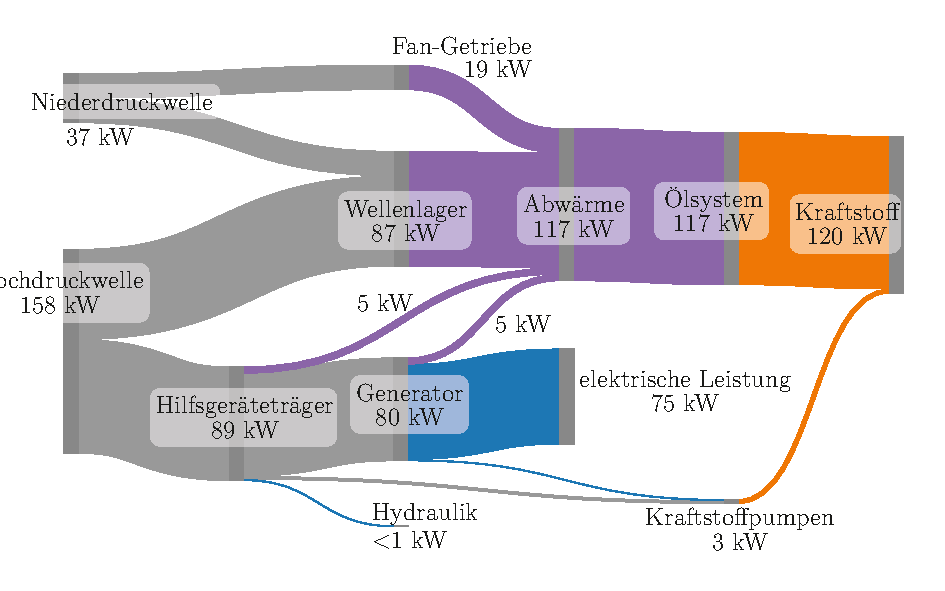
\includegraphics[width=1\linewidth]{4_Abbildungen/2_Hauptteil/sankey.pdf}
	\caption{Abwärmequellen des Kerosin-Kraftstoffsystems}
	\label{fig:sankey}
\end{figure}
\FloatBarrier 


Brewer \cite{Brewer.1991} hat für das Kabinen-Klimasystem (ECS) eines Schmalrumpfflugzeugs eine Abwärme pro Triebwerk von \SI{32}{\kilo\W} berechnet. Dieser Wert wird für die Modellierung übernommen. Durch das Kabinen-Klimasystem steht den Wasserstoff-Kraftstoffsystemen eine höhere Abwärme von insgesamt $\dot{Q}_{\mathrm{FOHE}}=$ \SI{149}{\kilo\W} zur Verfügung.

\section{Pumpen und Verdichter}

\subsection{Kreiselpumpen}

Kreiselpumpen kommen im Kerosin-Kraftstoffsystem als Niederdruckpumpe und im Wasserstoff-Kraftstoffsystem mit Pumpe als Hochdruckpumpe zum Einsatz. Kreiselpumpen erreichen ihren maximalen Wirkungsgrad bei mittleren Volumenströmen und hohen Druckverhältnissen, beziehungsweise Drehzahlen \cite{Gulich.2013}. %Ein typisches Kennfeld einer Kreiselpumpe ist in Abbildung \ref{fig:kreiselpumpe} dargestellt.

%\begin{figure}[ht]
%\centering
%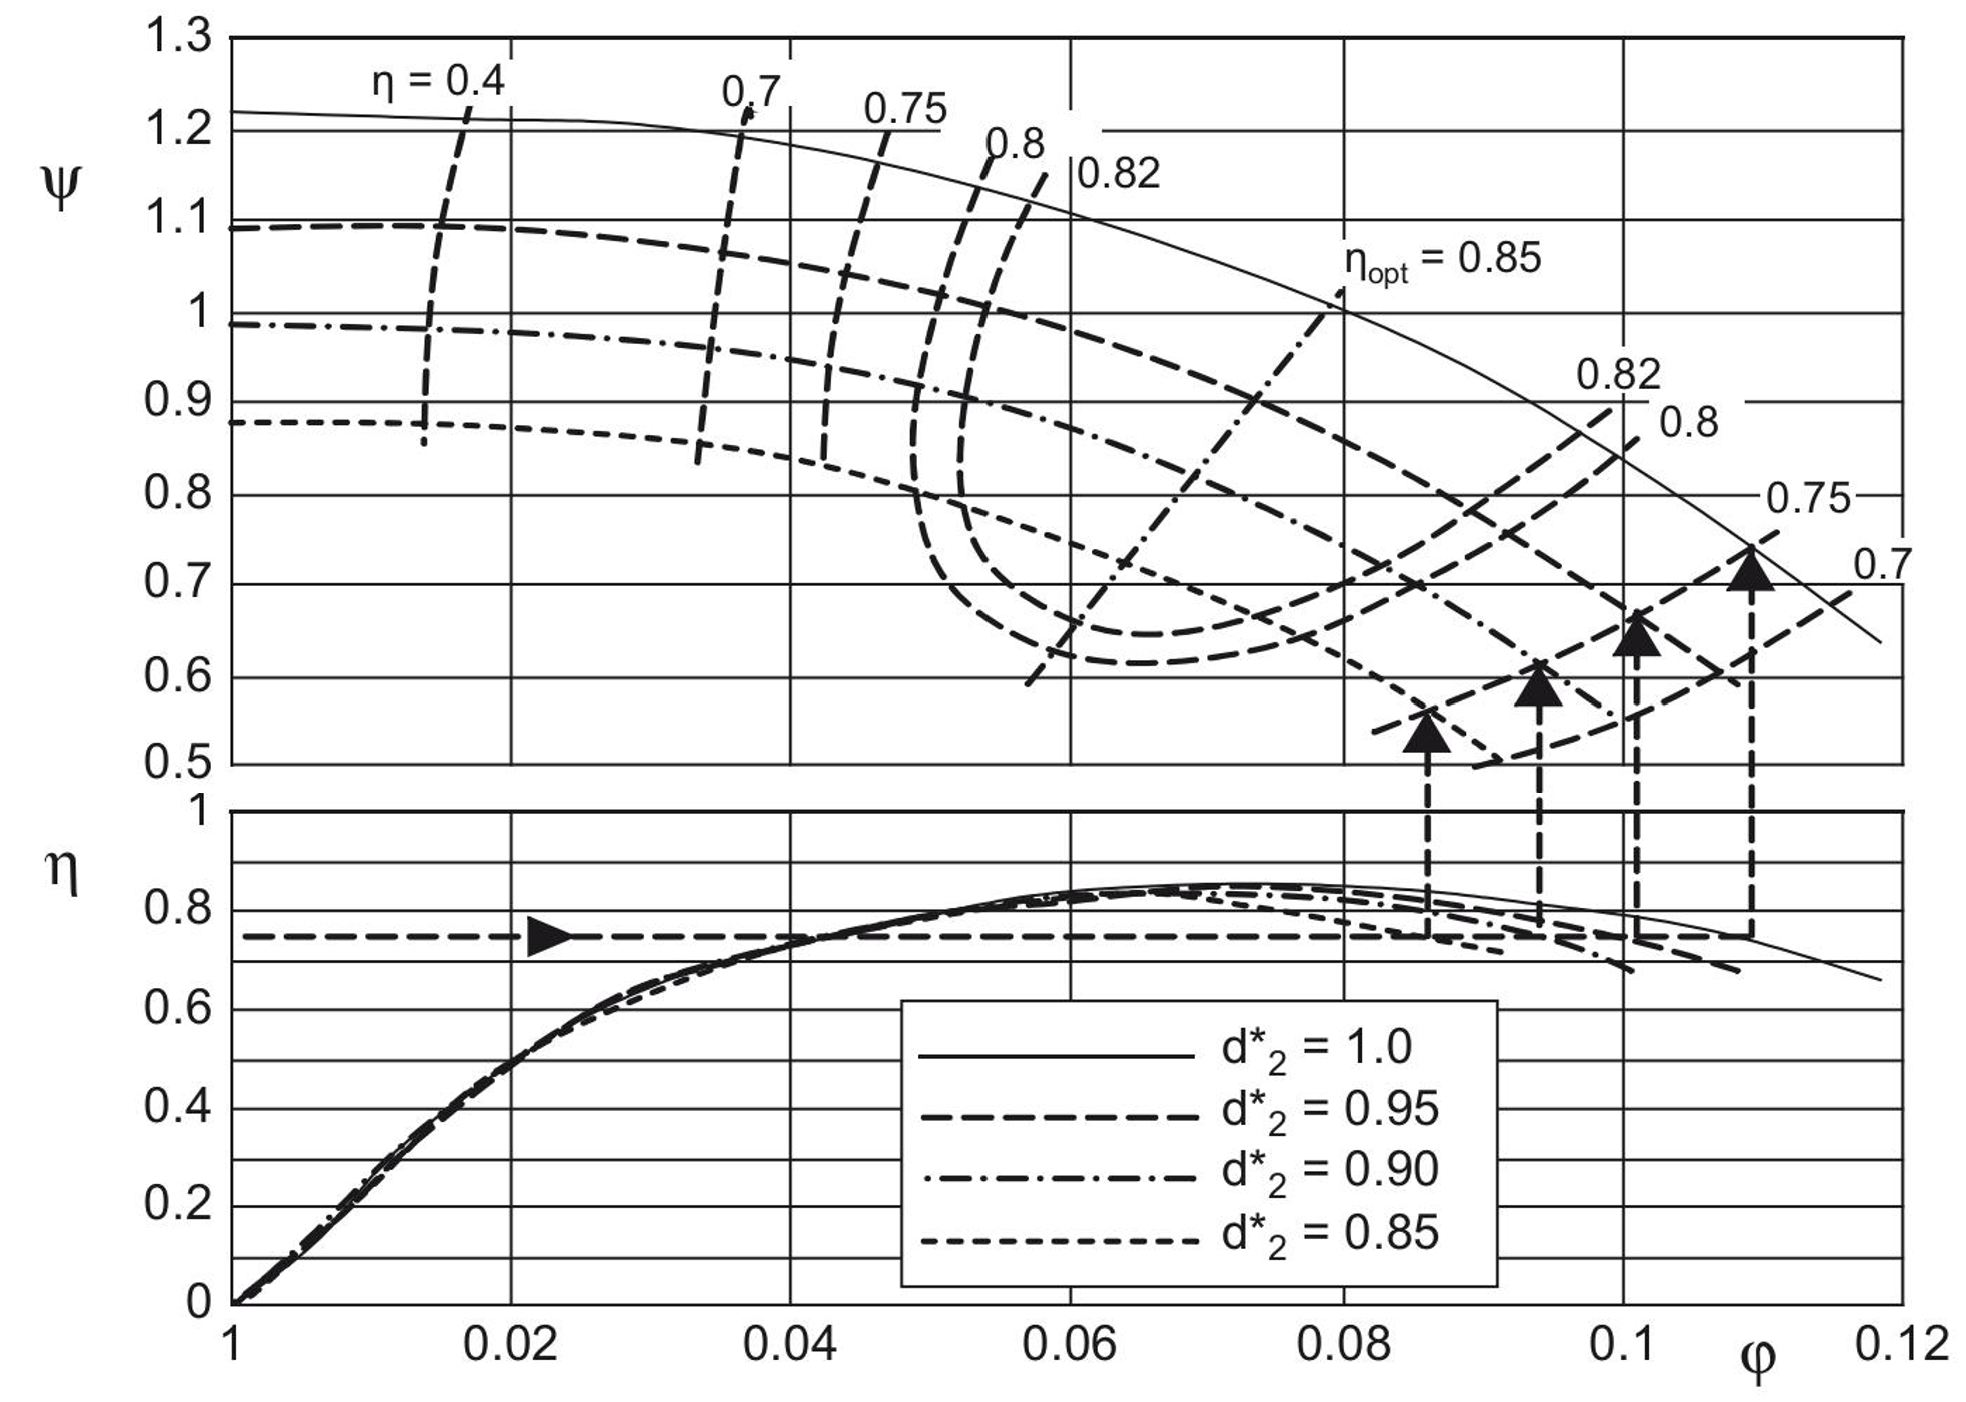
\includegraphics[width=0.8\linewidth]{4_Abbildungen/2_Hauptteil/kreiselpumpe.png}
%  \caption{Kennfeld einer Kreiselpumpe \cite{Gulich.2013}}
%  \label{fig:kreiselpumpe}
%\end{figure}
%\FloatBarrier 

Die Niederdruckpumpen von Kerosin-Kraftstoffsystemen erreichen im Reiseflug aufgrund der niedrigeren Drehzahlen und Volumenströmen im Vergleich zum optimalen Betriebspunkt nur vergleichsweise niedrige Wirkungsgrade zwischen $53$ und $66\,\%$ \cite{Zhou.2023}. Für die Niederdruckpumpe des Kerosin-Kraftstoffsystems wird ein isentroper Wirkungsgrad von $\eta_{\mathrm{LP}}=0,60$ angenommen. Die Niederdruckpumpe des CFM56-5B erzeugt im Auslegungspunkt eine Druckerhöhung von $\Delta p_{\mathrm{MTO}}=$ \SI{965}{\kilo\Pa}. Gemäß den Ähnlichkeitsbeziehungen für Pumpen \cite{Gulich.2013} beträgt der Austrittsdruck $p_{LP}$ 

\begin{equation}\label{Eq:lpfp}
	p_{\mathrm{LP}}=p_e+\Delta p_{\mathrm{MTO}}\left(\frac{N_2}{N_{2,\mathrm{MTO}}}\right)^2
\end{equation}

der Niederdruckpumpe im Reiseflug somit \SI{930}{\kilo\Pa}.

Da Wasserstoff-Kraftstoffsysteme keine nennenswerten Kraftstoffmassenströme in die Kraftstofftanks rückführen können, fallen die Volumenströme im Reiseflug relativ zu MTO-Bedingungen nochmals geringer aus als bei Kerosin-Kraftstoffsystemen. Brewer \cite{Brewer.1991} berechnet für den Wirkungsgrad einer Hochdruckpumpe mit konstanter Übersetzung im Wasserkraftstoffsystem einen Wert von $\eta_{\mathrm{HP}}=0,154$. Mit variabler Übersetzung sind höhere Wirkungsgrade möglich, jedoch verursachte diese Lösung höhere Betriebskosten und wird daher nicht betrachtet \cite{Brewer.1991}. 

\subsection{Zahnradpumpen}

Xu et al. \cite{Xu.2024} haben den Wirkungsgrad einer Zahnrad-Hochdruckpumpe bei unterschiedlichen Drehzahlen untersucht. Hohe Drehzahlen ermöglichen hohe Wirkungsgrade von bis zu $0,78$. Die Hochdruckpumpe des CFM56-5B arbeitet mit einer Nenndrehzahl von $6250$ 1/min \cite{EatonFuelSystemsDivision.2008}. Da die Hochdruckpumpe mit einem konstanten Übersetzungsverhältnis an die Hochdruckwelle angeschlossen ist, beträgt die Drehzahl im Reiseflug (mit $N_2/N_{2,\mathrm{MTO}}=0,88$) $5500$ 1/min. Interpolation der Daten von Xu et al. \cite{Xu.2024} ergibt somit einen Wirkungsgrad der Hochdruckpumpe von $\eta_{\mathrm{HP}}=0,73$.

Für die Hochdruckpumpe wird zudem der geförderte Massenstrom festgelegt. Unter MTO-Bedingungen fördert die Hochdruckpumpe den Kraftstoffverbrauch von \SI{1.05}{\kg\per\s} zuzüglich Kontingenz. Bei einem angenommenen Überschuss von $20\,\%$, beträgt der geförderte Massenstrom bei MTO-Schub \SI{1.27}{\kg\per\s}. Unter Annahme einer identischen volumetrischen Effizienz in beiden Lastpunkten beträgt der geförderte Massenstrom im Reiseflug aufgrund der niedrigeren Drehzahl somit $\dot{m}_\mathrm{HP}=$ \SI{1.11}{\kg\per\s}.

\subsection{Wasserstoff-Verdichter}

Der im Reiseflug gegenüber MTO-Bedingungen stark verringerte Volumenstrom bei nur geringfügig verringerter Drehzahl würde bei konstantem Übersetzungsverhältnis eine erhebliche Pumpgefahr bedeuten. Um einen stabilen Betrieb mit hohem Wirkungsgrad zu gewährleisten ist daher eine variable Übersetzung zwischen Verdichter und der Hochdruckwelle des Verdichters notwendig. 

Bei einem angenommenen Teillast-Wirkungsgrad des Verdichters von $0,75$ und einem mechanischen Wirkungsgrad der variablen Übersetzung von $0,95$ beträgt der Gesamtwirkungsgrad $\eta_{\mathrm{HP}}=\eta_\mathrm{RV}=0,71$.

\section{Wärmeübertrager Druckverluste}

Bei der Auslegung von Wärmeübertragern wird ein Kompromiss zwischen Bauvolumen/Masse und Druckverlust angestrebt. Da Masse und Bauvolumen der Kraftstoffsysteme in dieser Arbeit nicht berücksichtigt werden, erfolgt keine konkrete Auslegung der Wärmeübertrager, etwa mit der NTU-Methode. Stattdessen werden die Druckverluste anhand von Erfahrungswerten abgeschätzt. Für die Wasserstoff-Kraftstoffsysteme werden die Druckverluste in den Wärmeübertragern mit der parallelen Wasserstoffverbrennung, dem Kabinen-Klimasystem und dem Hauptölsystem sowie des Verdampfer bestimmt. Für das Kerosin-Kraftstoffsystem wird ausschließlich der Druckverlust im Wärmeübertrager des Hauptölsystem ermittelt.

\subsection{Kerosin-Kraftstoffsystem}

Zu den kraftstoffseitigen Druckverlusten in Wärmeübertragern von Kerosin-Kraftstoffsystemen liegen in der Literatur keine zuverlässigen Angaben vor, daher wird der Wert geschätzt. Einerseits sind bei Kerosin-Wärmeübertragern aufgrund der höheren Viskosität von Kerosin im Vergleich zu gasförmigem Wasserstoff sowie der geringeren Temperaturdifferenz der Fluidströme höhere Druckverluste zu erwarten. Andererseits überträgt der FOHE-Wärmeübertrager des Kerosin-Kraftstoffsystems aufgrund des höheren Massenstroms eine geringere spezifische Wärme als die der Wasserstoff-Kraftstoffsysteme. Zudem ermöglicht die deutlich höhere Dichte von Kerosin gegenüber gasförmigem Wasserstoff bei konstantem Flächen-zu-Massenstrom-Verhältnis niedrigere Strömungsgeschwindigkeiten, was geringere Druckverluste ermöglichen kann. Unter diesen Abwägungen wird für den FOHE-Wärmeübertrager des Kerosin-Kraftstoffsystems ein Druckverhältnis von $0,95$ angenommen.

\subsection{Wasserstoff-Kraftstoffsysteme}

Sciatti et al. \cite{Sciatti.2025} haben einen Wärmeübertrager zwischen Wasserstoff und Stickstoff untersucht und ausgelegt. Im Vergleich zum PHC-Wärmeübertrager der Wasserstoff-Kraftstoffsysteme dieser Arbeit sind die Temperaturdifferenz der Fluidströme geringer und die übertragene spezifische Wärme höher. Das von Sciatti et al. ermittelte Druckverhältnis über den Wärmeübertrager von $0,988$ stellt daher eine konservative Abschätzung der Druckverluste des PHC-Wärmeübertragers dar. Jedoch hat der ausgelegte Wärmeübertrager eine für den Wasserstoff-Massenstrom korrigierte Masse von \SI{111}{\kg} und ist damit inakzeptabel schwer. Für den PHC-Wärmeübertrager der Wasserstoff-Kraftstoffsysteme wird ein Druckverhältnis von $0,98$ angenommen.

Brewer \cite{Brewer.1991} hat für einen Wasserstoff Wärmeübertrager mit dem Kabinen-Klimasystem Druckverluste von \SI{2.14}{\kilo\Pa} berechnet. Die vernachlässigbar geringen Druckerverluste resultieren aus der geringen übertragenen Wärme bei moderater Temperaturdifferenz.

Für einen Wasserstoff-Wärmeübertrager mit dem Hauptölsystem hat Brewer ein Druckverhältnis von $0,984$ von berechnet \cite{Brewer.1991}. Die Wärmeübertrager mit den Hauptölsystemen der Wasserstoff-Kraftstoffsysteme dieser Arbeit übertragen das Vierfache der spezifischen Wärme. Die Übertragung der höheren spezifischen Wärme erfordert zusätzliche Rohrreihen im Wärmeübertrager. Da der Druckverlust unterproportional mit der Anzahl an Reihen skaliert \cite{.2013b}, erscheint ein Druckverhältnis über den Wärmeübertrager von $0,95$ realisierbar. Da die Druckverluste des Wärmeübertragers mit dem Klimasystem vernachlässigbar sind, ergibt sich für beide Wärmeübertrager in Summe ein Druckverhältnis von $\pi_{\mathrm{FOHE}}=0,95$.

Sciatti et al. \cite{Sciatti.2025} haben einen Wärmeübertrager für die Verdampfung von Flüssigwasserstoff mit erwärmtem Wasserstoff ausgelegt. Sie haben Druckverluste von \SI{5.74}{\Pa} für die heiße Seite und \SI{10.2}{\Pa} für die kalte Seite berechnet. Die vernachlässigbar geringen Druckverluste resultieren aus der hohen Temperaturdifferenz der Wasserstoff-Massenströme und der vergleichsweise geringen übertragenen Wärme. Für das Wasserstoff-Kraftstoffsystem mit Verdampfer werden daher die Druckverhältnisse $\pi_{\mathrm{V,LP}}=\pi_{\mathrm{V,HP}}=1$ angenommen.

\section{Leitungs- und Injektor-Druckverluste}

Die Leitungen der Kraftstoffsysteme verursachen Druckverluste infolge von Rohrreibung. Zudem erfordern die Injektoren eine minimale Druckdifferenz zwischen Kraftstoffzufuhr und Brennkammer, um eine adäquate Zerstäubung des Kraftstoffs zu gewährleisten.

\subsection{Kerosin-Kraftstoffsystem}

Die Rohrreibungsverluste im Kerosin-Kraftstoffsystem $\Delta p_\mathrm{L}$ 

\begin{equation}\label{Eq:dp}
	\Delta p_\mathrm{L}=\lambda\frac{L}{D}\frac{\rho}{2}v^2
\end{equation}

werden mit der Darcy-Weisbach-Gleichung bestimmt. Hierbei werden der Rohrreibungswert $\lambda=0,025$, die Leitungslänge $L=$ \SI{0.5}{\m}, der Leitungsdurchmesser $D=$ \SI{14}{\milli\m}, die Kraftstoffdichte $\rho=$ \SI{760}{\kg\per\m\cubed} und die Strömungsgeschwindigkeit $v=$ \SI{10}{\m\per\s} angenommen. Daraus resultiert der Druckverlust $\Delta p_\mathrm{L}=$ \SI{68}{\kilo\Pa}. 

Mazaheri et al. \cite{Mazaheri.2012} haben Drallinjektoren für Luftfahrtanwendungen mit einer Druckdifferenz von $\Delta p_{\mathrm{inj}}=$ \SI{300}{\kilo\Pa} ausgelegt.

\subsection{Wasserstoff-Kraftstoffsysteme}

Die Rohrreibungsverluste der Wasserstoff-Kraftstoffsysteme werden mit der Darcy-Weisbach-Gleichung (Gleichung \ref{Eq:dp}) bestimmt. Hierbei werden der Rohrreibungswert $\lambda=0,02$, die Leitungslänge $L=$ \SI{0.5}{\m}, der Leitungsdurchmesser $D=$ \SI{92}{\milli\m}, die Kraftstoffdichte $\rho=$ \SI{1.33}{\kg\per\m\cubed} und die Strömungsgeschwindigkeit $v=$ \SI{60}{\m\per\s} angenommen. Daraus resultiert der Druckverlust $\Delta p_\mathrm{L}=$ \SI{260}{\kilo\Pa}. 


Brewer \cite{Brewer.1991} hat für ein Wasserstoff-Kraftstoffsystem Injektor-Druckverluste von $p_{\mathrm{inj}}=$ \SI{169}{\kilo\Pa} berechnet. Dieser Wert wird für die Modellierung übernommen.

\section{Parallele Wasserstoffverbrennung}

Die parallele Wasserstoffverbrennung wird als magere Verbrennung mit einem Brennstoff-Luft-Verhältnis von 0,01 modelliert. Für die Verbrennung wird ein unterer Heizwert von Wasserstoff von $H_{u, \mathrm{H}_2}= $ \SI{120}{\mega\J\per\kg} angenommen. Die spezifischen isobaren Wärmekapazitäten von Luft und dem Abgas werden mit dem CEARUN Web-Tool \cite{Leader.} bestimmt. Für die Fan-Zapflufttemperatur wurde ein Wert von \SI{273}{\K} berechnet (Siehe Tabelle \ref{Tab:cruise}). Für die Annäherungstemperatur des PHC-Wärmeübertragers wird ein Wert von $\Delta T= $ \SI{30}{\K} angenommen. %Dieser Wert stellt einen Kompromiss zwischen der Masse des PHC-Wärmeübertragers und dem Gesamtwirkungsgrad dar.

\section{Zusammenfassung}

Die Parameter des Kerosin-Kraftstoffsystems sind in Tabelle \ref{Tab:referenz_parametrisiert} gesammelt.

\begin{table}[ht]
    \centering
	\caption{Randbedingungen des Kerosin-Kraftstoffsystems}
	\begin{tabular} {|l|c|c|c|c|} \hline%
		\multicolumn{2}{|c|}{Parameter} & Einheit & Wert & Quelle\\ \hline\hline%
        LPFP-Eintrittstemperatur & $T_e$ & K & 270 & - \\ \hline
        LPFP-Eintrittsdruck & $p_e$ & kPa & 180 & \cite{EatonFuelSystemsDivision.2013} \\ \hline
        FOHE-Wärme & $\dot{Q}_{\mathrm{FOHE}}$ & kW & 112 & - \\ \hline
        FOHE-Druckverhältnis & $\pi_{\mathrm{FOHE}}$ & - & 0,95 & - \\ \hline
        IDG-FOHE Wärme  & $\dot{Q}_\mathrm{IDG}$ & kW & 5 & \cite{Sciatti.2024} \\ \hline
        LPFP-Austrittsdruck & $p_\mathrm{LP}$ & kPa & 930 & - \\ \hline
        isentroper Wirkungsgrad LPFP & $\eta_\mathrm{LP}$ & - & 0,60 & \cite{Zhou.2023} \\ \hline
        isentroper Wirkungsgrad HPFP & $\eta_\mathrm{HP}$ & - & 0,73 & \cite{Xu.2024} \\ \hline
        HPFP-Massenstrom & $\dot{m}_\mathrm{HP}$ & kg/s & 1,11 & - \\ \hline
        Brennkammer-Massenstrom & $\dot{m}_\mathrm{BK}$ & kg/s & 0,313 & - \\ \hline
        Leitungs-Druckverluste & $\Delta p_\mathrm{L}$ & kPa & 68 & - \\ \hline
        Injektor-Druckverluste & $\Delta p_\mathrm{inj}$ & kPa & 300 & \cite{Mazaheri.2012} \\ \hline
	\end{tabular}	
    \label{Tab:referenz_parametrisiert}%
\end{table}
\FloatBarrier 

Die Parameter der Wasserstoff-Kraftstoffsysteme sind in Tabellen \ref{Tab:h2_parametrisiert} und \ref{Tab:h2_param2} dokumentiert.

\begin{table}[ht]
    \centering
	\caption{Parameter der Modellierungen aller Wasserstoff-Kraftstoffsysteme}
	\begin{tabular} {|l|c|c|c|c|} \hline%
    \multicolumn{5}{|c}{Alle Wasserstoff-Kraftstoffsysteme}\\ \hline
    \multicolumn{2}{|c|}{Parameter} & Einheit & Wert & Quelle\\ \hline\hline%
    isentroper Wirkungsgrad RV & $\eta_\mathrm{RV}$ & - & 0,71 & - \\ \hline
    Kraftstoff-Eintrittsdruck & $p_e$ & kPa & 345 & \cite{Brewer.1991, Scholz.2003} \\ \hline
    Kraftstoff-Eintrittstemperatur & $T_e$ & K & 25,2 & \cite{Brewer.1991, Scholz.2003} \\ \hline
    PHCHE-Druckverhältnis  & $\pi_\mathrm{PHC}$ & - & 0,98 & \cite{Sciatti.2025} \\ \hline
    FOHE-Wärme & $\dot{Q}_\mathrm{FOHE}$ & kW & 149 & - \\ \hline
    FOHE-Druckverhältnis & $\pi_\mathrm{FOHE}$ & - & 0,95 & \cite{Brewer.1991} \\ \hline
    Brennkammer-Massenstrom & $\dot{m}_{\mathrm{BK}}$ & kg/s & 0,110 & - \\ \hline
    Leitungs-Druckverluste & $\Delta p_\mathrm{L}$ & kPa & 260 & \cite{Brewer.1991} \\ \hline
    Injektor-Druckverluste & $\Delta p_\mathrm{inj}$ & kPa & 169 & \cite{Brewer.1991} \\ \hline
    PHC-Brennstoff-Luft-Verhältnis & $\beta_\mathrm{PHC}$ & - & 0,01 & - \\ \hline
    isobare Wärmekapazität Luft & $c_{p, \mathrm{L}}$ & \si{\kilo\J\per\kg\per\K} & 1,0 & \cite{Leader.} \\ \hline
    isobare Wärmekapazität Abgas & $c_{p, \mathrm{B}}$ & \si{\kilo\J\per\kg\per\K} & 1,1 & \cite{Leader.} \\ \hline
    unterer Heizwert Wasserstoff & $H_{u, \mathrm{H}_2}$ & MJ/kg & 120 & - \\ \hline
    PHCHE-Annäherungstemperatur & $\Delta T$ & K & 30 & - \\ \hline
    Fan-Zapflufttemperatur & $T_{13}$ & K & 273 & - \\ \hline
   
    \end{tabular}	
    \label{Tab:h2_parametrisiert}%
\end{table}
\FloatBarrier 

\begin{table}[ht]
	\centering
	\caption{Parameter der Modellierungen der einzelnen Wasserstoff-Kraftstoffsysteme}
	\begin{tabular} {|l|c|c|c|c|} \hline%	
		\multicolumn{5}{|c|}{Architektur mit Hochdruckpumpe}\\ \hline
		\multicolumn{2}{|c|}{Parameter} & Einheit & Wert & Quelle\\ \hline\hline%
		isentroper Wirkungsgrad HPFP & $\eta_\mathrm{HP}$ & - & 0,154 & \cite{Brewer.1991} \\ \hline
		\multicolumn{5}{|c|}{Architektur mit Verdampfer}\\ \hline
		\multicolumn{2}{|c|}{Parameter} & Einheit & Wert & Quelle\\ \hline\hline%
		isentroper Wirkungsgrad HPFC & $\eta_\mathrm{HP}$ & - & 0,71 & - \\ \hline
		Druckverhältnis LP-Verdampfer & $\pi_\mathrm{V,LP}$ & - & 1 & \cite{Sciatti.2025} \\ \hline
		Druckverhältnis HP-Verdampfer & $\pi_\mathrm{V,HP}$ & - & 1 & \cite{Sciatti.2025} \\ \hline\hline
		\multicolumn{5}{|c|}{Architektur mit Vormischung}\\ \hline
		\multicolumn{2}{|c|}{Parameter} & Einheit & Wert & Quelle\\ \hline\hline%
		isentroper Wirkungsgrad HPFC & $\eta_\mathrm{HP}$ & - & 0,71 & - \\ \hline
	\end{tabular}	
	\label{Tab:h2_param2}%
\end{table}
\FloatBarrier 

\section{Brennkammereintritts-Bedingungen}

Im Folgenden werden die unabhängigen Variablen, also die Brennkammer-Eintrittsbedingungen der Kraftstoffsysteme, erläutert. Zunächst wird der Brennkammerdruck der Kraftstoffsysteme festgelegt. Anschließend wird die zulässige Brennkammer-Eintrittstemperatur für das Kerosin-Kraftstoffsystem bestimmt. Zuletzt werden denkbare Wertebereiche für die Betrachtung der Brennkammer- und Wärmeübertrager-Eintrittstemperaturen der Wasserstoff-Kraftstoffsysteme in einer Parameterstudie bestimmt.

\subsection{Brennkammerdruck}

Der Brennkammerdruck beträgt sowohl für das Kerosin- als auch die Wasserstoff-Kraftstoffsysteme $p_\mathrm{BK}=p_3=$ \SI{1330}{\kilo\Pa} (siehe Tabelle \ref{Tab:cruise}).

\subsection{Brennkammer-Eintrittstemperatur Kerosin-Kraftstoffsystem}

Um im Kerosin-Kraftstoffsystem geringere Brennkammer-Eintrittstemperatur zu erreichen, muss eine größere Menge an Kraftstoff in die Kraftstofftanks rückgeführt werden. Um den rückgeführten Kraftstoff zu ersetzen fördert die Niederdruckpumpe einen höheren Kraftstoffmassenstrom, was ihren Leistungsbedarf steigert. Aus diesem Grund wird eine möglichst hohe Brennkammer-Eintrittstemperatur angestrebt. 

Der Brennkammer-Eintrittstemperatur ist jedoch durch die maximal zulässige Öltemperatur eine technische Obergrenze gesetzt. Der Kraftstoff kann nur bis zu der maximalen Öltemperatur abzüglich der Annäherungstemperatur des Wärmeübertragers erhitzt werden. Bei dem PW1133G Triebwerk beträgt die maximale Öltemperatur im Reiseflug \SI{419}{\K} \cite{EASA.2018}. Bei einer angenommenen Annäherungstemperatur zuzüglich Kontingenz von \SI{20}{\K} beträgt die maximal zulässige Brennkammer-Eintrittstemperatur somit $T_\mathrm{BK}=$ \SI{399}{\K}.

\subsection{Eintrittstemperaturen Wasserstoff-Kraftstoffsysteme}

Das EnableH2 Projekt \cite{Patrao.2023} sowie Brewer \cite{Brewer.1991} gehen von Brennkammer-Eintrittstemperaturen von über \SI{650}{\K} aus. Diese hohen Temperaturen erreichen die Autoren insbesondere durch den Einsatz von Wärmerückgewinnung aus dem Abgas des Kerntriebwerks. Die Autoren des CRYOPLANE Berichts \cite{Scholz.2003} und der Joint Cryogenic Engine Study \cite{SIMON.1994} halten Wasserstofftemperaturen von \SI{150}{\K} für ausreichend. Tacconi et al. \cite{Tacconi.2023} haben für ihre Betrachtung eines Wasserstoff-Kraftstoffsystems eine minimale akzeptable Temperatur von \SI{273}{\K} angenommen, um Probleme infolge von Vereisung in der Brennkammer zu vermeiden. Aufgrund der breiten Palette an Vorschlägen für Brennkammer-Eintrittstemperaturen für Wasserstoff-Kraftstoffsysteme wird diese Variable in der Parameterstudie in einem Wertebereich zwischen $150$ und \SI{500}{\K} untersucht. Für den Vergleich mit dem Kerosin-Kraftstoffsystem wird ein Wert von \SI{300}{\K} verwendet.

Ähnliches gilt für die Wärmeübertrager-Eintrittstemperatur. Um Vereisungen in den Öl- und Luftwärmeübertragern zu vermeiden, wird eine minimale Eintrittstemperatur gewahrt. Wärmeübertrager-Eintrittstemperaturen oberhalb des Gefrierpunkts von Wasser sind jedoch nicht sinnvoll, da dort keine Vereisungsgefahr mehr besteht und eine weitere Erhöhung der Temperatur lediglich den rezirkulierten Massenstrom erhöhen würde. Der Wärmeübertrager-Eintrittstemperatur ist jedoch durch die Brennkammer-Eintrittstemperatur eine weitere Obergrenze gesetzt. Damit exzessive rezirkulierte Massenströme vermieden werden, wird stets eine Wärmeübertrager-Eintrittstemperatur gewählt, die mindestens \SI{20}{\K} unter der Brennkammer-Eintrittstemperatur liegt. Die Wärmeübertrager-Eintrittstemperatur wird im Rahmen der Parameterstudie in einem Wertebereich zwischen $100$ und \SI{280}{\K} untersucht. Für den Vergleich mit dem Kerosin-Kraftstoffsystem wird ein Wert von \SI{160}{\K} verwendet.

						
%==============================================================================
\chapter{Ergebnisse} \label{chap:ergebnis}
%==============================================================================

In diesem Kapitel werden mit der vorgeschlagenen Modellierung berechneten Ergebnisse diskutiert. Dabei steht insbesondere die Frage im Fokus, ob die Modellierung den Leistungs- und Wärmebedarf der Kraftstoffsysteme akkurat vorhersagen kann. Hierfür wird im Rahmen einer Sensitivitätsanalyse die Auswirkung von Unsicherheiten der in Kapitel \ref{chap:param} bestimmten Parametern auf das Modellverhalten untersucht. Danach wird die Methodik dieser Arbeit mit Daten aus der Literatur validiert. Anschließend wird im Rahmen einer Parameterstudie analysiert, wie sich die Eintrittstemperaturen des Kraftstoffs in den ersten Wärmeübertrager und die Brennkammer auf die Modellierungen der Wasserstoff-Kraftstoffsysteme auswirkt. Abschließend erfolgt ein Vergleich des Leistungs- und Wärmebedarfs der H$_2$-Kraftstoffsysteme untereinander und mit dem Kerosin-Kraftstoffsystem anhand eines ausgewählten Betriebspunkts.

\section{Sensitivitätsanalyse}

Im Folgenden wird eine Sensitivitätsanalyse durchgeführt und ausgewertet, um die für das Modellverhalten maßgeblichen Parameter zu identifizieren. Zunächst werden hierfür die Unsicherheiten der Parameter geschätzt. Anschließend werden die mit Unsicherheit behafteten Parameter in die Modellierungen der Kraftstoffsysteme eingesetzt, um die Abweichungen Leistungsbedarfe zu berechnen.

\subsection{Bestimmung der Schrittweiten}

Da die statistische Verteilung der Parameterwerte nicht bekannt ist, werden die Schrittweiten für die Variation der Parameter geschätzt. Die Schrittweiten werden so gewählt, dass die Abweichung der Pumpenleistung des H$_2$-Kraftstoffsystems mit Verdampfer stets ein positives Vorzeichen aufweist.

Der Austrittsdruck der Niederdruckpumpe $p_\mathrm{LPFP}$ des Kerosin-Kraftstoffsystems ist stets höher als der Öldruck im Wärmeübertrager des Hauptölsystems und somit von diesem abhängig. Der Öldruck ist eine Funktion der Druckverlust des Ölsystems. Aus diesem Grund wird eine moderate Schrittweite von $-10\,\%$ gewählt.

Da die Druckverluste von Wärmeübertragern und Leitungen ein Auslegungsziel darstellen, sind sie nicht direkt mit Unsicherheit behaftet. Jedoch können abweichende Anforderungen an das Gewicht dieser Komponenten eine Aufweichung der Auslegungsziele erfordern. Um diesen Effekt zu berücksichtigen werden der Leitungsdruckverlust $\Delta p_L$ und die Druckverluste $1-\pi_i$ der Wärmeübertrager mit einer Schrittweite von $+20\,\%$ variiert. 

Die Druckverluste des Verdampfers $1-\pi_{\mathrm{V}, i}$ werden in der Modellierung des Kraftstoffsystems vernachlässigt. Da auf der Hochdruckseite zwar geringe, jedoch im Verhältnis zur Niederdruckseite höhere Druckverluste zu erwarten sind (Siehe Kapitel \ref{chap:param}), werden absolute Schrittweiten von $+0,01$ auf der Hochdruckseite und $+0,005$ auf der Niederdruckseite verwendet. 

Die Unsicherheiten der Wirkungsgrade von Pumpen und Verdichtern $\eta_i$, der verfügbaren Abwärme $\dot{Q}_\mathrm{FOHE}$  und den Injektor-Druckverlusten $\Delta p_\mathrm{inj}$ werden als gering eingeschätzt. Aus diesem Grund wird für diese Parameter eine Schrittweite von $\pm 5\,\%$ ausgewählt.

\subsection{Auswertung der Sensitivitätsanalyse}

Auf Basis der zuvor bestimmten Schrittweiten wird im Folgenden die Sensitivität der Kraftstoffsysteme untersucht und ausgewertet. Zunächst werden die Ergebnisse der Modellierung des H$_2$-Kraftstoffsystems mit Verdampfer präsentiert. Daraufhin werden die Ergebnisse der Sensitivitätsanalysen der H$_2$-Kraftstoffsysteme miteinander verglichen. Abschließend werden die Ergebnisse der Sensitivitätsanalyse für das Kerosin-Kraftstoffsystem diskutiert.

Die Ergebnisse der Sensitivitätsanalyse für das H$_2$-Kraftstoffsystem mit Verdampfer sind in Tabelle \ref{Tab:sensjeta} dargestellt.

\begin{table}[ht]
	\centering
	\caption{Sensitivitätsanalyse des H$_2$-Kraftstoffsystems mit Verdampfer}
	\begin{tabular} {|l|c|c|c|c|c|} \hline%
		Parameter & Einheit & Schrittweite & Schrittweite [\%] & $ \Delta \sum P_i$ [\%] \\ \hline\hline%
		$\Delta p_\mathrm{L}$ & \si{\kilo\Pa} & +52,0 & +20,0 & +5,39 \\ \hline 
		$1-\pi_\mathrm{FOHE}$ & - & +0,010 & +20,0 & +1,98 \\ \hline 
		$1-\pi_\mathrm{PHC}$ & - & +0,004 & +20,0 & +0,768 \\ \hline
		$\eta_\mathrm{HPFC}$ & - & -0,0355 & -5,00 & +2,68 \\ \hline  
		$\eta_\mathrm{RV}$ & - & -0,0355 & -5,00 & +1,71 \\ \hline 
		$\dot{Q}_\mathrm{FOHE}$ & \si{\kilo\W} & -7,95 & -5,00 & +0,0541 \\ \hline 
		$\Delta p_\mathrm{inj}$ & \si{\kilo\Pa} & +8,45 & +5,00 & +0,0829 \\ \hline 
		$1-\pi_\mathrm{V, HP}$ & - & +0,010 & - & +1,88 \\ \hline 
		$1-\pi_\mathrm{V, LP}$ & - & +0,005 & - & +0,202 \\ \hline 
	\end{tabular}	
	\label{Tab:sensafter}%
\end{table}
\FloatBarrier 

Mit einem Anstieg der Leistungen um  $+5,39\,\%$ hat die Erhöhung der Leitungs-Druckverluste bei Weitem die größte Auswirkung auf die Modellierung des H$_2$-Kraftstoffsystems mit Verdampfer. Die Reduktionen der Wirkungsgrade der Verdichter haben mit $+2,68\,\%$ (Hochdruckverdichter) beziehungsweise $+1,71\,\%$ (Rezirkulationsverdichter) nur eine moderate Auswirkung auf die Verdichterleistungen. 

Die Erhöhungen der Druckverluste des Ölsystem-Wärmeübertragers und der Hochdruckseite des Verdampfers führen mit $1,98\,\%$ und $1,88\,\%$ ebenfalls zu moderaten anstiegen der Leistungen. Hingegen hat der Anstieg der Druckverluste des PHC-Wärmeübertragers und der Niederdruckseite des Verdampfers nur geringen Einfluss auf die Leistungen. 

Ein Anstieg der Injektor-Druckverluste hat nur geringe Auswirkungen auf die Verdichter-Leistungen.


Die Tabellen \ref{Tab:senspump} und \ref{Tab:sensdual} zeigen die Ergebnisse der Sensitivitätsanalysen für die H$_2$-Kraftstoffsysteme mit Hochdruckpumpe und Vormischung.

\begin{table}[ht]
	\centering
	\caption{Sensitivitätsanalyse des H$_2$-Kraftstoffsystems mit Pumpe}
	\begin{tabular} {|l|c|c|c|c|c|} \hline%
		Parameter & Referenzwert & Einheit & Schrittweite & $ \Delta \sum P_i$ [\%] \\ \hline\hline%
		$\dot{Q}_\mathrm{FOHE}$ & 149000,0 & \si{\kilo\W} & -7,45 & +0,0511 \\ \hline 
		$1-\pi_\mathrm{FOHE}$ & 0,95 & - & +0,010 & +3,00 \\ \hline 
		$1-\pi_\mathrm{PHC}$ & 0,98 & - & +0,004 & +1,17 \\ \hline 
		$\eta_\mathrm{RV}$ & 0,71 & - & -0,040 & +3,35 \\ \hline 
		$\eta_\mathrm{HPFP}$ & 0,154 & - & -0,008 & +1,47 \\ \hline 
		$\Delta p_\mathrm{L}$ & 260000,0 & \si{\kilo\Pa} & +52,0 & +8,19 \\ \hline 
		$\Delta p_\mathrm{inj}$ & 169000,0 & \si{\kilo\Pa} & +8,45 & -0,054 \\ \hline 
	\end{tabular}	
	\label{Tab:senspump}%
\end{table}
\FloatBarrier 

\begin{table}[ht]
	\centering
	\caption{Sensitivitätsanalyse des H$_2$-Kraftstoffsystems mit Vormischung}
	\begin{tabular} {|l|c|c|c|c|c|} \hline%
		Parameter & Einheit & Schrittweite & Schrittweite [\%] & $ \Delta \sum P_i$ [\%] \\ \hline\hline%
		$\Delta p_\mathrm{L}$ & \si{\kilo\Pa} & +52,0 & +20,0 & +5,38 \\ \hline 
		$1-\pi_\mathrm{FOHE}$ & - & +0,010 & +20,0 & +1,97 \\ \hline 
		$1-\pi_\mathrm{PHC}$ & - & +0,004 & +20,0 & +0,766 \\ \hline
		$\eta_\mathrm{HPFC}$ & - & -0,0355 & -5,00 & +2,68 \\ \hline  
		$\eta_\mathrm{RV}$ & - & -0,0355 & -5,00 & +1,70 \\ \hline 
		$\dot{Q}_\mathrm{FOHE}$ & \si{\kilo\W} & -7,95 & -5,00 & +0,0551 \\ \hline 
		$\Delta p_\mathrm{inj}$ & \si{\kilo\Pa} & +8,45 & +5,00 & +0,0838 \\ \hline 
	\end{tabular}	
	\label{Tab:sensdual}%
\end{table}
\FloatBarrier 

Die H$_2$-Kraftstoffsysteme weisen nur geringfügige Unterschiede in ihren Sensitivitäten auf. Das H$_2$-Kraftstoffsystem mit Hochdruckpumpe zeigt mit $+8,19\,\%$ eine besonders hohe Sensitivität gegenüber Variationen der Leitungs-Druckverluste. Auch Änderungen der Druckverluste in den Wärmeübertragern haben einen stärkeren Einfluss auf dieses System. Die Ergebnisse des H$_2$-Kraftstoffsystems mit Vormischung weichen nur minimal von denen des H$_2$-Kraftstoffsystems mit Verdampfer ab.

Die Ergebnisse der Sensitivitätsanalyse für das Kerosin-Kraftstoffsystem sind in Tabelle \ref{Tab:sensjeta} zusammengefasst.

\begin{table}[ht]
	\centering
	\caption{Sensitivitätsanalyse des Kerosin-Kraftstoffsystems}
	\begin{tabular} {|l|c|c|c|c|} \hline%
		Parameter & Einheit & Schrittweite & Schrittweite [\%] & $ \Delta \sum P_i$ [\%] \\ \hline\hline%
		$p_\mathrm{LPFP}$ & - & -93,0 & -10,0 & +4,38 \\ \hline 
		$\Delta p_\mathrm{L}$ & \si{\kilo\Pa} & +13,6 & +20,0 & +1,21 \\ \hline 
		$1-\pi_\mathrm{FOHE}$ & - & +0,010 & +20,0 & +0,828 \\ \hline 
		$\eta_\mathrm{HPFP}$ & - & -0,0365 & -5,00 & +3,81 \\ \hline 
		$\eta_\mathrm{LPFP}$ & - & -0,030 & -5,00 & +1,48 \\ \hline 
		$\dot{Q}_\mathrm{FOHE}$ & \si{\kilo\W} & -6,35 & -5,20 & -1,36 \\ \hline 
		$\Delta p_\mathrm{inj}$ & \si{\kilo\Pa} & +30,0 & +10,0 & +2,67 \\ \hline 
	\end{tabular}	
	\label{Tab:sensjeta}%
\end{table}
\FloatBarrier 

Zwar führt der verringerte Austrittsdruck zu einer geringeren Leistung der Niederdruckpumpe, jedoch steigt hierdurch das Druckverhältnis und die Leistung der Hochdruckpumpe. Die Auswirkungen auf die Hochdruckpumpe überwiegen, was zu einem Anstieg des Leistungsbedarfs um $4,38\,\%$ führt – der größten Abweichung unter den Parametern. 

Eine Verringerung des Wirkungsgrads der Hochdruckpumpe hat einen um $3,81\,\%$ höheren Leistungsbedarf zur Folge. Aufgrund des geringeren Leistungsbedarfs der Niederdruckpumpe hat die Variation ihres Wirkungsgrads mit $1,48\,\%$ eine geringere Auswirkung. 

Eine Steigerung der Injektor-Druckverluste führt zu einem um $2,67\,\%$ höheren Leistungsbedarf der Pumpen. Im Vergleich haben die Variation der Leitungs- und Wärmeübertrager-Druckverluste einen geringen Einfluss auf den Leistungsbedarf. 

Die kleinere Abwärme führt zu einem geringeren Massenstrom durch die Niederdruckpumpe und somit zu einer um $1,36\,\%$ verringerten Pumpenleistung.

\section{Validierung}

Zur Validierung der Methodik dieser Arbeit wird das Wasserstoff-Kraftstoffsystem mit Pumpe angepasst und parametriert, um das von Brewer \cite{Brewer.1991} vorgeschlagene Kraftstoffsystem nachzuempfinden. 

Dabei werden folgende Modifikationen an der Modellierung vorgenommen: Die Druckverluste im rezirkulierten Kraftstoffstrom werden vernachlässigt, da das Kraftstoffsystem nach Brewer keinen Rezirkulationsverdichter vorsieht. Der Kraftstoffmassenstrom wird nicht an die Brennkammer-Eintrittstemperatur angepasst und eine parallele Wasserstoffverbrennung ist nicht vorgesehen. Zudem bleibt der Wärmeeintrag des von Brewer vorgeschlagenen Rekuperators unberücksichtigt, da sich dieser Wärmeübertrager Stromabwärts der Entnahmestelle des rezirkulierten Kraftstoffs befindet - eine Konfiguration, die von der Modellierung dieser Arbeit abweicht. Um dennoch eine Vergleichbarkeit der Pumpenleistung zu gewährleisten, wird der Druckverlust dieses Wärmeübertragers zu den Druckverluste der Injektoren addiert. 

Ein weiterer Unterschied liegt in der Modellierung des Kraftstoffs: Während in dieser Arbeit Parawasserstoff verwendet wird, basieren Brewers Berechnungen auf Normalwasserstoff. Dies macht eine Anpassung der Modellparameter des Wasserstoff-Stoffmodels erforderlich. Tabelle \ref{Tab:brewer} zeigt die weiteren Änderungen der Parameter und Variablen gegenüber dem ursprünglichen Wasserstoff-Kraftstoffsystem mit Pumpe.

\begin{table}[ht]
    \centering
	\caption{Veränderte Parameter der Validierung}
	\begin{tabular} {|l|c|c|c|} \hline%
    \multicolumn{2}{|c|}{Parameter} & Einheit & Wert\\ \hline\hline%
    FOHE Druckverhältnis & $\pi_\mathrm{FOHE}$ & - & 1 \\ \hline
    Brennkammer-Massenstrom & $\dot{m}_\mathrm{BK}$ & kg/s & 0,166 \\ \hline
    Leitungsdruckverluste & $\Delta p_\mathrm{r}$ & kPa & 30 \\ \hline
    Injektordruckverluste & $\Delta p_\mathrm{inj}$ & kPa & 214,4 \\ \hline
    Brennkammer-Eintrittsdruck & $p_\mathrm{BK}$ & kPa & 1516,2 \\ \hline
    Brennkammer-Eintrittstemperatur & $T_\mathrm{BK}$ & K & 264 \\ \hline
    Wärmeübertrager-Eintrittstemperatur & $T_\mathrm{W}$ & K & 200 \\ \hline
    \end{tabular}	
    \label{Tab:brewer}%
\end{table}
\FloatBarrier 

Tabelle \ref{Tab:validation} zeigt die von Brewer berechneten Werte und die mit der beschriebenen Methodik berechneten Werte. 

\begin{table}[ht]
    \centering
	\caption{Validierung der Methodik}
	\begin{tabular} {|l|c|c|c|c|} \hline%
    \multicolumn{2}{|c|}{Variable} & Einheit & Brewer \cite{Brewer.1991} & Diese Arbeit \\ \hline\hline%
    Pumpenleistung & $P_\mathrm{HPFP}$ & kW & 23,9 & 23,4 \\ \hline
    Wärme & $\dot{Q}$ & kW & 542,7 & 539,8 \\ \hline
    Rezirkulierter Massenstrom & $\dot{m}_\mathrm{R}$ & kg/s & 0,377 & 0,439 \\ \hline
    Pumpen-Austrittstemperatur & $T_{2,\mathrm{HPFP}}$ & K & 50 & 33,1 \\ \hline
    \end{tabular}	
    \label{Tab:validation}%
\end{table}
\FloatBarrier 

Die Werte für die Pumpenleistung und den Wärmebedarf stimmen weitgehend mit den Berechnungen von Brewer überein. Allerdings berechnet Brewers einen um $14\,\%$ geringeren rezirkulierten Massenstrom, was auf die um \SI{16.9}{\K} höhere Pumpen-Austrittstemperatur mit seinem Modell zurückzuführen ist. Um den Ursprung dieser Abweichung zu identifizieren, wird die Energiebilanz verwendet. Die Energiebilanz um die Hochdruckpumpe des Brewer-Konzepts 

\begin{equation}\label{Eq:brewer}
	\Delta \dot{E}_\mathrm{HPFP}=\dot{m}_\mathrm{BK}(h(T_0,p_0)-h(T_\mathrm{HPFP}, p_\mathrm{HPFP}))+P_\mathrm{HPFP}
\end{equation}

weist ein Residuum von $\Delta \dot{E}_\mathrm{HPFP}=$ \SI{-79.9}{\kilo\W} auf. Ähnliche Energiebilanzen für die Wasserstoffmischung und die Wärmeübertrager ergeben Residuen von $\Delta \dot{E}_\mathrm{mix}=$ \SI{25.3}{\kilo\W} und $\Delta \dot{E}_\mathrm{W}=$ \SI{57.2}{\kilo\W}. Da das Residuum der Energiebilanz des gesamten Kraftstoffsystems mit $\Delta \dot{E}=$ \SI{2.3}{\kilo\W} gering ist, erscheint ein Fehlerursprung im verwendeten Stoffmodell als unwahrscheinlich. Die Abweichungen auf Komponenten-Ebene könnten durch einen nicht dokumentierten Wärmeübertrager zwischen flüssigem und verdampften Wasserstoff erklärt werden. Aufgrund dieser Problematik ist eine belastbare Validierung der Methodik dieser Arbeit nicht möglich.

\section{Parameterstudie}

Um die Wechselwirkung zwischen Wärmeübertrager- und Brennkammer-Eintrittstemperatur auf die Betriebsmittelbedarfe der Wasserstoff-Kraftstoffsysteme zu untersuchen wird eine zweidimensionale Parameterstudie durchgeführt. Die Parameter und Konfiguration der Wasserstoff-Kraftstoffsysteme werden über den untersuchten Bereich als konstant angenommen. Da sich die Wasserstoff-Kraftstoffsysteme untereinander in ihrem Verhalten weitgehend ähneln, werden die Ergebnisse zunächst für die Architektur mit Hochdruckpumpe gezeigt. Anschließend werden die Unterschiede zwischen den Architekturen im Detail betrachtet.

\subsection{Architektur mit Hochdruckpumpe}

Abbildung \ref{fig:pumppower} zeigt den mechanischen Leistungsbedarf des Wasserstoff-Kraftstoffsystems mit Pumpe für den untersuchten Temperaturbereich. 

\begin{figure}[ht]
\centering
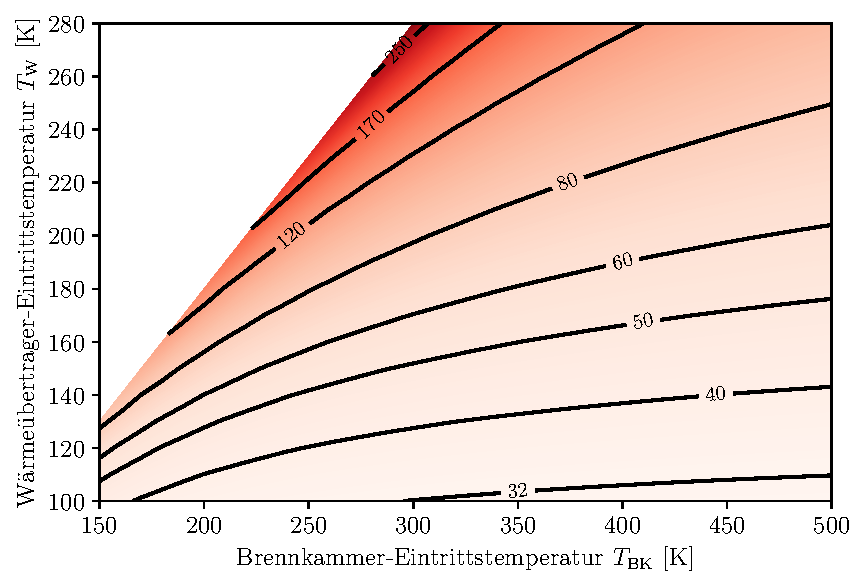
\includegraphics[width=0.9\linewidth]{4_Abbildungen/2_Hauptteil/Ergebnisse/Pumpepowercontour.pdf}
  \caption{Leistungsbedarf Wasserstoff-Kraftstoffsystem mit Pumpe [kW]}
  \label{fig:pumppower}
\end{figure}
\FloatBarrier

Der Gesamtleistungsbedarf steigt mit zunehmender Wärmeübertrager-Eintrittstemperatur, da die geringe Differenz zur Brennkammer-Eintrittstemperatur einen größeren Rezirkulations-Massenstrom erfordert, was die Leistung des Rezirkulationsverdichters erhöht. Zwar führen höhere Brennkammer-Eintrittstemperaturen zu einer Zunahme der spezifischen Arbeit des Rezirkulationsverdichters, jedoch wird dieser Effekt durch den aufgrund der erhöhten Temperaturdifferenz reduzierten rezirkulierten Massenstrom mehr als ausgeglichen. Die Leistung der Hochdruckpumpe ist hingegen unabhängig von den Eintrittstemperaturen (Abbildung \ref{fig:pumpsplit}). 

\begin{figure}[ht]
\centering
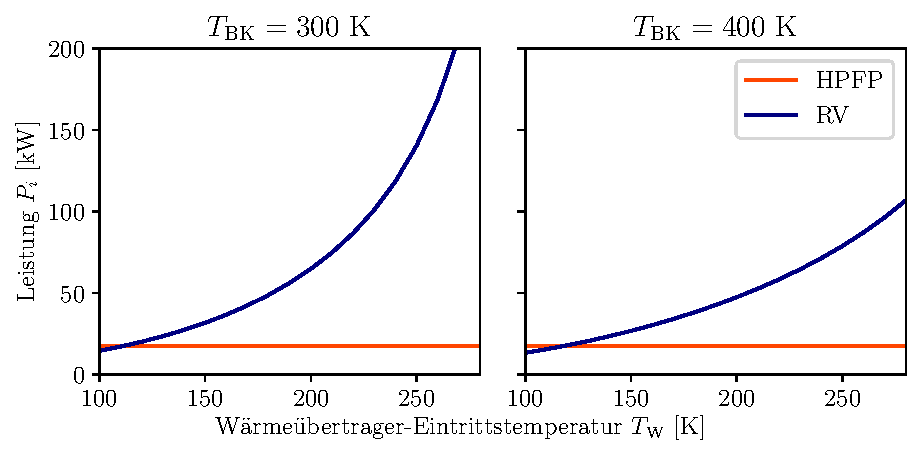
\includegraphics[width=0.9\linewidth]{4_Abbildungen/2_Hauptteil/Ergebnisse/Pumpe_powersplit.pdf}
  \caption{Leistungsaufteilung Architektur mit Pumpe}
  \label{fig:pumpsplit}
\end{figure}
\FloatBarrier

Der Wärmebedarf ist insbesondere mit der Brennkammer-Eintrittstemperatur korreliert. Da die Leistung des Rezirkulationsverdichters mit steigender Wärmeübertrager-Eintrittstemperatur beziehungsweise geringer Differenz der Eintrittstemperaturen zunimmt, liegt in diesem Fall ein verringerter Wärmebedarf vor. Dieses Verhalten ist in Abbildung \ref{fig:pumpheat} dargestellt.

\begin{figure}[ht]
\centering
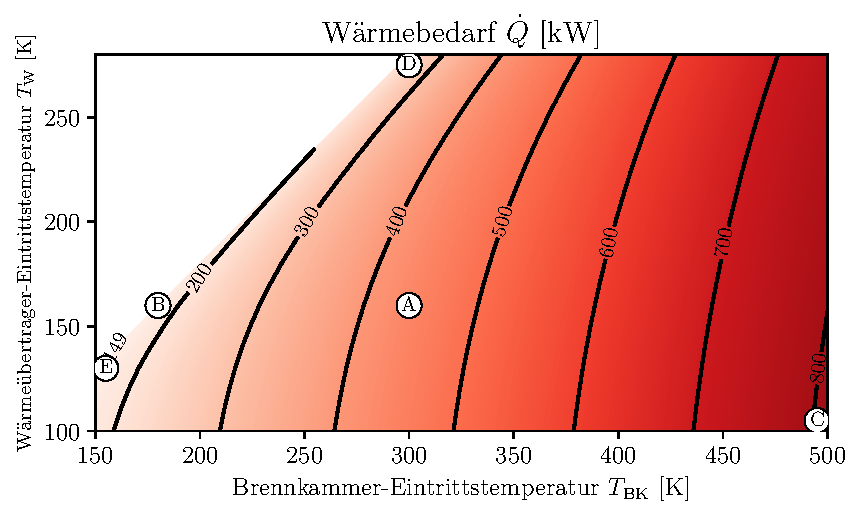
\includegraphics[width=0.9\linewidth]{4_Abbildungen/2_Hauptteil/Ergebnisse/Pumpeheatcontour.pdf}
  \caption{Wärmebedarf Wasserstoff-Kraftstoffsystem mit Pumpe [kW]}
  \label{fig:pumpheat}
\end{figure}
\FloatBarrier

Abbildung \ref{fig:pumpfuel} zeigt den Kraftstoffverbrauch des Triebwerks mit dem Kraftstoffsystem mit Pumpe für die unterschiedlichen Eintrittstemperaturen.

\begin{figure}[ht]
\centering
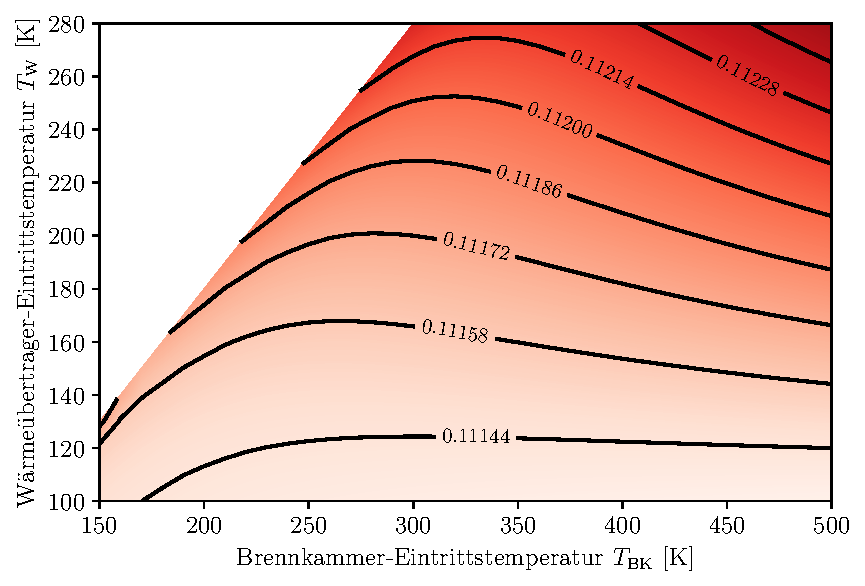
\includegraphics[width=0.9\linewidth]{4_Abbildungen/2_Hauptteil/Ergebnisse/Pumpemassflowcontour.pdf}
  \caption{Kraftstoffverbrauch Wasserstoff-Kraftstoffsystem mit Pumpe [kg/s]}
  \label{fig:pumpfuel}
\end{figure}
\FloatBarrier

Die Leistung des Rezirkulationsverdichters bei hohen Wärmeübertrager-Eintritts-temperaturen verringert den Gesamtwirkungsgrad des Triebwerks. Im Gegensatz dazu hat die Brennkammer-Eintrittstemperatur einen geringeren Einfluss auf den Verbrauch.


\subsection{Vergleich der Wasserstoff-Kraftstoffsysteme}

Im Folgenden werden die Ergebnisse der Parameterstudie für die verschiedenen Wasserstoff-Kraftstoffsysteme miteinander verglichen. Abbildung \ref{fig:comp_power} zeigt den Leistungsbedarf der Kraftstoffsysteme in Abhängigkeit der Wärmeübertrager-Eintrittstemperatur für zwei verschiedene Brennkammer-Eintrittstemperaturen.

\begin{figure}[ht]
\centering
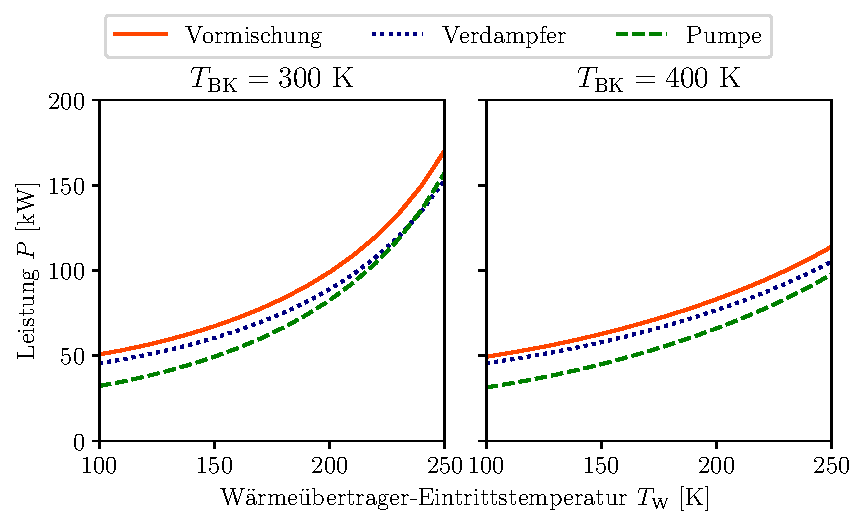
\includegraphics[width=0.9\linewidth]{4_Abbildungen/2_Hauptteil/Ergebnisse/summary_power.pdf}
  \caption{Leistungsbedarf Wasserstoff-Kraftstoffsysteme}
  \label{fig:comp_power}
\end{figure}
\FloatBarrier

Aufgrund der höheren spezifischen Arbeit der Verdichtung im gasförmigen Zustand weisen beide Verdichterarchitekturen im Vergleich zur Pumpenarchitektur einen erhöhten Leistungsbedarf auf. Da die Verdichter des Kraftstoffsystems mit Vormischung bei identischer spezifischer Arbeit einen größeren Massenstrom  fördern als die Verdichter der Architektur mit Verdampfer, hat das Kraftstoffsystem mit Vormischung einen höheren Leistungsbedarf. Dieser Effekt wird bei höheren Brennkammer-Eintrittstemperaturen abgeschwächt, da die Verdampfung in diesem Fall einen geringeren Massenstrom erfordert. Abbildung \ref{fig:comp_split} zeigt den Einfluss der Wärmeübertrager-Eintrittstemperatur auf die Komponenten-Leistungen.

\begin{figure}[ht]
\centering
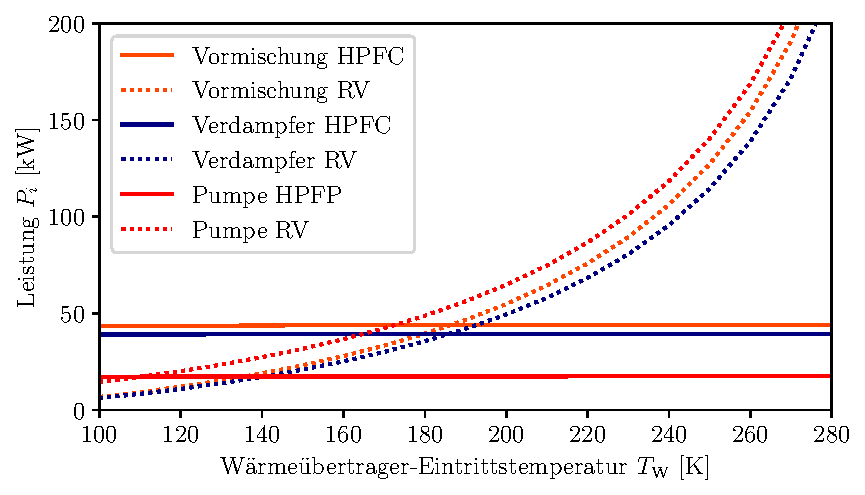
\includegraphics[width=0.9\linewidth]{4_Abbildungen/2_Hauptteil/Ergebnisse/300summary_powersplit.pdf}
  \caption{Leistungsaufteilung Vergleich [$T_\mathrm{BK}=$ \SI{300}{\K}]}
  \label{fig:comp_split}
\end{figure}
\FloatBarrier

Analog zur Architektur mit Pumpe hat die Wärmeübertrager-Eintrittstemperatur bei den Verdichterarchitekturen keinen Einfluss auf die Leistung des Hochdruckverdichters. Da die Verdichterarchitekturen im Vergleich zur Pumpenarchitektur einen geringeren Rezirkulationsmassenstrom aufweisen, fällt auch die Leistung des Rezirkulationsverdichters geringer aus. Abbildung \ref{fig:tbk_split} zeigt den Einfluss der Brennkammer-Eintrittstemperatur auf die Komponenten-Leistungen.

\begin{figure}[ht]
\centering
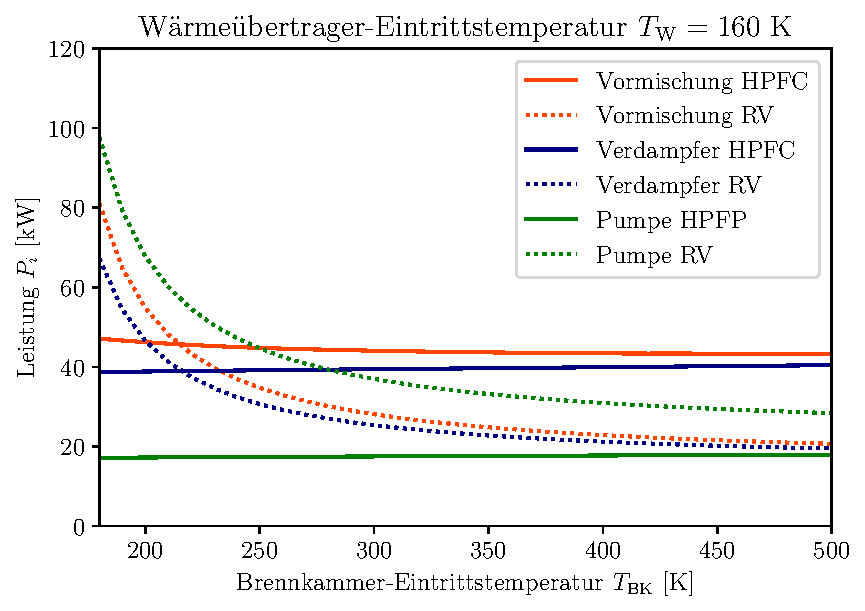
\includegraphics[width=0.7\linewidth]{4_Abbildungen/2_Hauptteil/Ergebnisse/tbkcomp.pdf}
  \caption{Leistungsaufteilung Vergleich [$T_\mathrm{W}=$ \SI{160}{\K}]}
  \label{fig:tbk_split}
\end{figure}
\FloatBarrier

Der Trend sinkender Leistung des Rezirkulationsverdichters bei höherer Differenz der Eintrittstemperaturen setzt sich auch bei den Verdichterarchitekturen fort. Im Gegensatz zu den anderen Architekturen führen steigende Brennkammer-Eintrittstemperaturen bei der Architektur mit Vormischung jedoch zu einer geringfügigen Reduzierung der Leistung des Hochdruckverdichters. Dies ist auf den geringeren erforderlichen Massenstrom für die Verdampfung zurückzuführen. 

Abbildung \ref{fig:stackplot} gibt einen Überblick der Leistungsanteile der Wasserstoff-Kraftstoffsysteme. In der linken Spalte sind die Leistungsanteile in Abhängigkeit der Brennkammereintritts-Temperatur bei konstanter Wärmeübertrager-Eintrittstemperatur dargestellt. Die mittlere Spalte zeigt die Leistungsanteile in Abhängigkeit der Brennkammer-Eintrittstemperatur, aber mit konstanter Temperaturdifferenz. Die rechte Spalte zeigt die Leistungsanteile in Abhängigkeit der Wärmeübertrager-Temperatur bei konstanter Brennkammereintritts-Eintrittstemperatur.

\begin{figure}[ht]
\centering
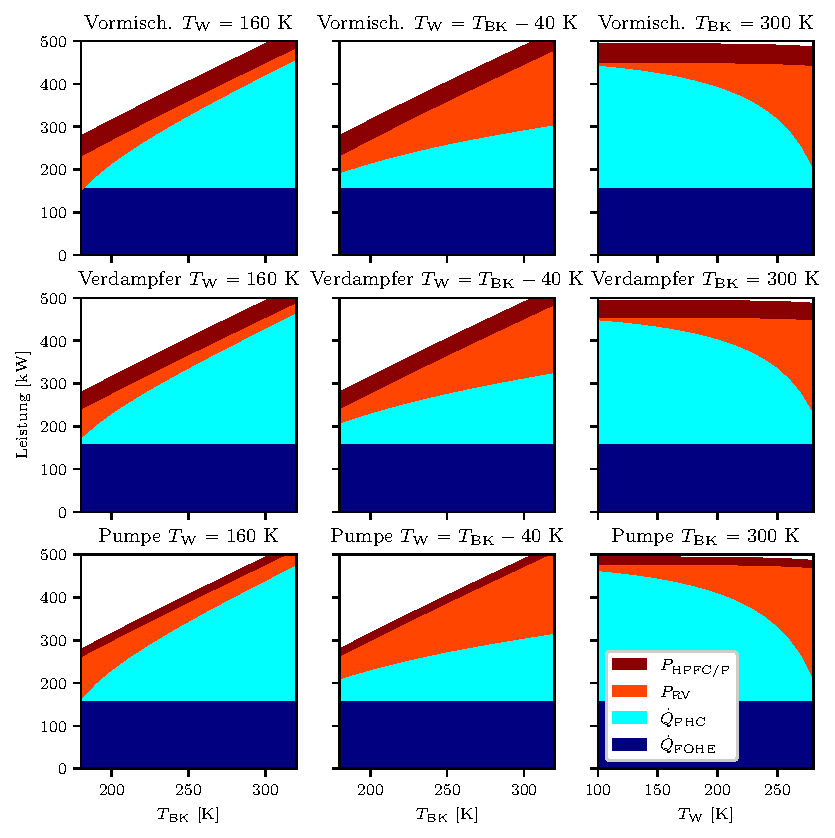
\includegraphics[width=1\linewidth]{4_Abbildungen/2_Hauptteil/Ergebnisse/stackplot_summary.pdf}
  \caption{Stapeldiagramme der Leistungsanteile}
  \label{fig:stackplot}
\end{figure}
\FloatBarrier

Diese Abbildung verdeutlicht den Einfluss der Differenz der Eintrittstemperaturen. Bei einer konstanten Temperaturdifferenz von $T_{BK}-T_W=$ \SI{40}{\K} (mittlere Spalte) liegen die Leistung des Rezirkulationsverdichters $P_{RV}$ und die Wärme der parallelen Wasserstoffverbrennung $\dot{Q}_{PHC}$ über die untersuchten Brennkammer-Eintrittstemperaturen betragsmäßig in einem ähnlichen Bereich. Im Gegensatz dazu nimmt bei konstanter Brennkammer-Eintrittstemperatur der Leistungsanteil des Rezirkulationsverdichters mit steigender Wärmeübertrager-Eintrittstemperatur zu (rechte Spalte).

Eine direkte Empfehlung spezifischer Eintrittstemperaturen lässt sich aus diesen Daten nicht ableiten. Grundsätzlich gilt, dass eine möglichst niedrige hinnehmbare Wärmeübertrager-Eintrittstemperatur den Kraftstoffverbrauch reduziert. Für die Brennkammer-Eintrittstemperatur lässt sich hingegen keine eindeutige Aussage treffen, sodass sie in Abhängigkeit von der Wärmeübertrager-Eintrittstemperatur gewählt werden sollte.

\section{Vergleich Kerosin- und Wasserstoff-Kraftstoffsysteme}

Im Folgenden werden die Wasserstoff-Kraftstoffsysteme mit dem Kerosin-Kraftstoffsystem verglichen. Abbildung \ref{fig:refcomp} zeigt den Betriebsmittelbedarf der verschiedenen Kraftstoffsysteme. Für die Wasserstoff-Kraftstoffsysteme gilt eine Brennkammer-Eintrittstemperatur von $T_\mathrm{BK}=$ \SI{300}{\K} und eine Wärmeübertrager-Eintrittstemperatur von $T_\mathrm{W}=$ \SI{160}{\K}.

\begin{figure}[ht]
\centering
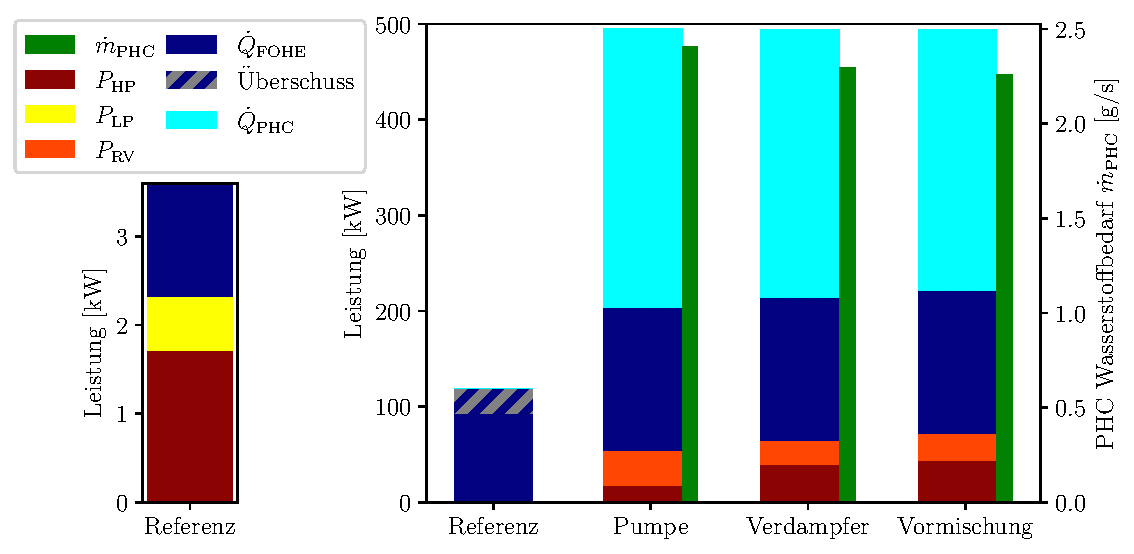
\includegraphics[width=1\linewidth]{4_Abbildungen/2_Hauptteil/Ergebnisse/refcomp.pdf}
  \caption{Betriebsmittelbedarf der Kraftstoffsysteme}
  \label{fig:refcomp}
\end{figure}
\FloatBarrier

Der Betriebsmittelbedarf der Wasserstoff-Kraftstoffsysteme übersteigt den Bedarf des Kerosin-Kraftstoffsystems um einen Faktor von drei. Im Vergleich zum Kerosin-Kraftstoffsystem erfordert das Wasserstoff-Kraftstoffsystem mit Pumpe 22,7-Mal mehr Leistungsentnahme von der Hochdruckwelle und hat einen Wärmefehlbetrag von \SI{278}{\kilo\W}, der durch die parallele Wasserstoffverbrennung gedeckt wird. Bei dem Kraftstoffsystem mit Verdampfer wird sogar das 27,1-Fache an Leistungsentnahme benötigt bei einem Wärmefehlbetrag von \SI{268}{\kilo\W}. Bei dem Kraftstoffsystem mit Vormischung wird das 30,2-Fache an Leistungsentnahme benötigt bei einem Wärmefehlbetrag von nur noch \SI{261}{\kilo\W}. 

Um die Vergleichbarkeit des Kraftstoffverbrauchs sicherzustellen, wird der Energieverbrauch als Produkt aus dem Kraftstoffverbrauch und dem unteren Heizwert bei Normaldruck und einer Temperatur von \SI{298.15}{\K} berechnet.
Abbildung \ref{fig:refenergy} zeigt die Differenz des Energieverbrauchs der Wasserstoff-Kraftstoffsysteme zum Kerosin-Kraftstoffsystem. 

\begin{figure}[ht]
\centering
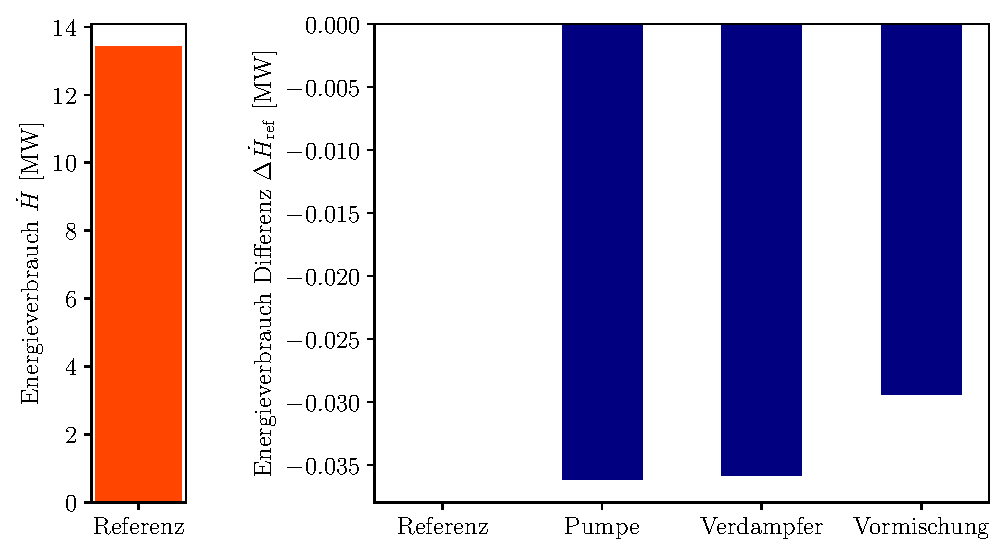
\includegraphics[width=1\linewidth]{4_Abbildungen/2_Hauptteil/Ergebnisse/refenergy.pdf}
  \caption{Energieverbrauch der Kraftstoffsysteme}
  \label{fig:refenergy}
\end{figure}
\FloatBarrier

Trotz des zusätzlichen Betriebsmittelbedarfs verbrauchen die Wasserstoff-Kraftstoffsysteme bis zu $0{,}27\,\%$ weniger Energie. Dies ist auf den höheren Wirkungsgrad des Kreisprozesses des wasserstoffbetriebenen Zyklus zurückzuführen, der durch die abweichenden Abgaseigenschaften begünstigt wird.
%==============================================================================
\chapter{Zusammenfassung und Ausblick}
\label{chap:fazit}
%==============================================================================

Der Einsatz wasserstoffbetriebener Fluggasturbinen erfordert Leistungsfähige Kraftstoffsysteme, die den erheblichen Wärmebedarf für die Vorkonditionierung des flüssigen Wasserstoffs decken können. Kenntnis der spezifischen Wärme- und Leistungsanforderungen in den relevanten Betriebspunkten ist dabei essenziell für die angemessene Dimensionierung der Systemkomponenten. Der Fokus dieser Arbeit ist die Entwicklung einer Modellierung zur Abschätzung dieser Anforderungen, insbesondere in Abhängigkeit der durch die Systemauslegung zu bestimmenden Eintrittstemperaturen. 

Im Rahmen dieser Arbeit wurden ein Referenzkraftstoffsystem und drei Wasserstoff-Kraftstoffsysteme entwickelt. Die Modellierung der Kraftstoffsysteme erfolgte anhand von Komponenten- und Stoffmodellen, die auf Basis einer umfassenden Literaturrecherche für den Betriebspunkt eines Verkehrsflugzeugs im Reiseflug parametriert wurden. Diese Modellierung bestimmt den Wärmebedarf, die erforderlichen Pumpen- und Verdichterleistungen sowie den daraus resultierenden Mehrverbrauch in Abhängigkeit von den Auslegungsgrößen.  Zudem ermöglichen die zugrunde liegenden Komponenten- und Stoffmodelle eine flexible Kombination in verschiedenen Anordnungen, um alternative Kraftstoffsystem-Konzepte abzubilden und zu vergleichen.

Die Methodik dieser Arbeit wurde auf ein bekanntes Kraftstoffsystem aus der Literatur angewandt, um die Aussagekraft des Ansatzes zu bestätigen. Das Ergebnis dieser Validierung ergab eine Übereinstimmung mit den Literaturdaten, jedoch nur in Teilen. Der Ursprung dieser Abweichung konnte nicht abschließend geklärt werden. Im Rahmen einer zweidimensionalen Parameterstudie der Wasserstoff-Kraftstoffsysteme konnte ein Zusammenhang zwischen Kraftstoffverbrauch und Wärmeübertrager-Eintrittstemperatur festgestellt werden. In dem Anschließenden Vergleich mit dem Referenzkraftstoffsystem konnte gezeigt werden, dass die Wasserstoff-Kraftstoffsysteme im Reiseflug trotz höherem Wärmebedarf und höherer notwendiger Leistungsentnahme einen geringeren Energieverbrauch ermöglichen. 

Zukünftige Arbeiten könnten sich mit abweichenden Anordnungen der Komponenten der Wasserstoff-Kraftstoffsysteme befassen, insbesondere im Hinblick auf die Integration von Wärmeübertragern und der Rezirkulation, um die Wärmeübertrager-Eintrittstemperatur zu erreichen. Fortgeschrittene Arbeiten könnten sich damit beschäftigen die Modellierung auf Gesamttriebwerksebene in Leistungsrechnungen zu integrieren und die Modellierung durch die Berücksichtigung von transienten und Off-Design-Punkten zu erweitern. Dies würde zudem die Entwicklung einer Regelstrategie für die einzelnen Kraftstoffsystemkomponenten erfordern.



%%% c) Literaturverzeichnis																					
\renewcommand{\baselinestretch}{0.90}\normalsize
\urlstyle{same}
\bibliographystyle{natdin}
\bibliography{Literatur}
\addcontentsline{toc}{chapter}{Literatur}


%%% d) Anhang
%\renewcommand{\baselinestretch}{1.00}\normalsize
%\appendix




%%% d) ToDo-Notes
%\listoftodos																%% Erstellt Liste mit Aufgaben. Zum deaktivieren in der Datei Pakete.tex zwischen den eckigen Klammern disable hinzufügen

\end{document}